% ------------------------------------------------------------------------
% ------------------------------------------------------------------------
% ICMC: Modelo de Trabalho Acadêmico (tese de doutorado, dissertação de
% mestrado e trabalhos monográficos em geral) em conformidade com 
% ABNT NBR 14724:2011: Informação e documentação - Trabalhos acadêmicos -
% Apresentação
% ------------------------------------------------------------------------
% ------------------------------------------------------------------------

% Opções: 
%   Qualificação          = qualificacao 
%   Curso                 = doutorado/mestrado
%   Situação do trabalho  = pre-defesa/pos-defesa (exceto para qualificação)
%   Versão para impressão = impressao
\documentclass[mestrado, pre-defesa]{packages/icmc}

% ---------------------------------------------------------------------------
% Pacotes Opcionais
% ---------------------------------------------------------------------------
\usepackage{rotating}           % Usado para rotacionar o texto
\usepackage[all,knot,arc,import,poly]{xy}   % Pacote para desenhos gráficos
% Este pacote pode conflitar com outros pacotes gráficos como o ``pictex''
% Então é necessário usar apenas um dos pacotes conflitantes
\newcommand{\VerbL}{0.52\textwidth}
\newcommand{\LatL}{0.42\textwidth}
% ---------------------------------------------------------------------------


% ---
% Informações de dados para CAPA e FOLHA DE ROSTO
% ---
% Tanto na capa quanto nas folhas de rosto apenas a primeira letra da primeira palavra (ou nomes próprios) devem estar em letra maiúscula, todas as demais devem ser em letra minúscula.
\tituloPT{Estudo do impacto econômico de uma pandemia utilizando dados de Documentos Fiscais}
\tituloEN{Study of the economic impact of a pandemic using Invoices}
\autor[Miguel, L. A.]{Leonardo Alves Miguel}
\genero{M} % Gênero do autor (M = Masculino / F = Feminino)
\orientador[Orientador]{Prof. Dr.}{Francisco Aparecido Rodrigues}
%\coorientador{Prof. Dr.}{Fulano de Tal}
\curso{MECAI}
\data{28}{01}{2021} % Data do depósito
\idioma{PT} % Idioma principal do documento (PT = português / EN = inglês)
% ---


% ---
% RESUMOS
% ---

% Resumo em PORTUGUÊS
% conter no máximo 500 palavras
% conter no mínimo 1 e no máximo 5 palavras-chave
\textoresumo[brazil]{
    Um resumo
    }{Algumas, palavras, chave}


% resumo em INGLÊS
% conter no máximo 500 palavras
% conter no mínimo 1 e no máximo 5 palavras-chave
\textoresumo[english]{
    A abstract
    }{Some, keywords}


% ----------------------------------------------------------
% ELEMENTOS PRÉ-TEXTUAIS
% ----------------------------------------------------------

% Inserir a ficha catalográfica
\incluifichacatalografica{tex/pre-textual/ficha-catalografica.pdf}

% DEDICATÓRIA / AGRADECIMENTO / EPÍGRAFE
\textodedicatoria*{tex/pre-textual/dedicatoria}
\textoagradecimentos*{tex/pre-textual/agradecimentos}
\textoepigrafe*{tex/pre-textual/epigrafe}

% Inclui a lista de figuras
\incluilistadefiguras

% Inclui a lista de tabelas
\incluilistadetabelas

% Inclui a lista de quadros
\incluilistadequadros

% Inclui a lista de algoritmos
\incluilistadealgoritmos

% Inclui a lista de códigos
\incluilistadecodigos

% Inclui a lista de siglas e abreviaturas
\incluilistadesiglas

% Inclui a lista de símbolos
\incluilistadesimbolos

% Dependências inseridas pelo autor
\usepackage{multirow}

% ----
% Início do documento
% ----
\begin{document}
% ----------------------------------------------------------
% ELEMENTOS TEXTUAIS
% ----------------------------------------------------------
\textual

\chapter{Introdução}
\label{chapter:introducao}
% Comando simples para exibir comandos Latex no texto
\newcommand{\comando}[1]{\textbf{$\backslash$#1}}

Segundo dados da \citeonline{receita:dados-publicos:cnpj}, o Brasil possuía em setembro de 2020 mais de 45 milhões de empresas ativas que realizam transações todos os dias envolvendo aquisição e transferência de mercadorias, prestação de serviços das mais diversas naturezas, transportes e devoluções. Essas empresas possuem uma série de obrigações contábeis e fiscais a cumprir todos os meses. Obrigações essas que se traduzem em documentos enviados ao governo contendo uma série de informações sobre cada uma dessas transações efetuadas.

A lei que obriga a emissão de notas fiscais é datada do ano de 1994~\cite{lei:8846:documentos-fiscais}. À época, a emissão desses documentos era feita em papel, o que causava grandes transtornos às empresas tanto por conta dos próprios processos envolvidos quanto por conta da guarda desses documentos.

outros trabalhos relacionados a estudo de documentos fiscais

outras analises do impacto economico da pandemia

Na seção~\ref{chapter:documenos-fiscais} será apresentado o domínio dos dados utilizados neste trabalho com uma explicação sobre documentos fiscais, a legislação brasileira envolvida, e os sistemas usados para captação dos dados. Em seguida, na seção~\ref{chapter:pandemia} será introduzido todo o contexto da Pandemia de COVID-19 e a sequência de eventos envolvida que, além de causar uma grave crise sanitária de dimensões mundiais, teve também seus impactos econômicos. A seguir, será descrita a base de dados utilizada com uma análise descritiva e detalhes do pré-processamento feito para a coleta dos dados na seção~\ref{chapter:base-de-dados}. Completar...


\chapter{Documentos Fiscais}
\label{chapter:documenos-fiscais}

A legislação fiscal brasileira é notoriamente conhecida por ser complexa. Nas duas últimas décadas, representantes das três esferas do governo brasileiro, municipal, estadual, e federal, se reuniram para tentar mudar essa realidade promovendo uma atuação mais integrada e modernizando o sistema. O mercado brasileiro também respondeu a essas mudanças criando oportunidades que visam facilitar o cumprimento das obrigações fiscais de empresas de todo país.

\section{Legislação Brasileira}

O Sistema Tributário Nacional foi instituído pela lei nº 5172 de 1966 \cite{lei:1966:codigo_tributario}, há mais de cinco décadas. Desde então passou por diversas reformas visando aumentar sua eficiência, modernizando-o. O artigo 37 da Constituição Federal, alterado pela Emenda Constitucional nº 42 de 19 de dezembro de 2003 \cite{constituicao:emenda42_2003}, em seu vigésimo segundo inciso prevê:

\begin{citacao}
Art. 37. A administração pública direta e indireta de qualquer dos Poderes da União, dos Estados, do Distrito Federal e dos Municípios obedecerá aos princípios de legalidade, impessoalidade, moralidade, publicidade e eficiência e, também, ao seguinte:

...

XXII - as administrações tributárias da União, dos Estados, do Distrito Federal e dos Municípios, atividades essenciais ao funcionamento do Estado, exercidas por servidores de carreiras específicas, terão recursos prioritários para a realização de suas atividades e atuarão de forma integrada, inclusive com o compartilhamento de cadastros e de informações fiscais, na forma da lei ou convênio \cite{constituicao:1988}.
\end{citacao}

O compartilhamento de cadastros e de informações previsto neste artigo permitiu então que as esferas do governo brasileiro tomassem atitudes no sentido de centralizar sistemas tributários, criando protocolos e sistemas para tal.

Desde então, diversos secretários da Fazenda Federal, das Fazendas Estaduais e do Distrito Federal, e de Fazendas Municipais se reúnem anualmente no \sigla{ENAT}{Encontro Nacional de Administradores Tributários} para discutir como modernizar e tornar mais efetivo o Sistema Tributário Brasileiro. A seguir, são descritos alguns importantes protocolos assinados nesses encontros.

\subsection{ENAT}

Em julho de 2004, em Salvador-BA, ocorre a primeira edição do ENAT. Neste encontro, foram assinados dois protocolos de cooperação  técnica para a instalação do Projeto Cadastro Sincronizado e do Projeto de Escrituração Digital.

No protocolo de Projeto Cadastro Sincronizado, fica previsto a construção de um cadastro de contribuintes sincronizado seguindo as seguintes diretivas:

\begin{citacao}
Na construção do cadastro referido na cláusula primeira, serão observados os seguintes parâmetros, entre outros que vierem a ser definidos de comum acordo pelos partícipes:

I - entrada de dados única;

II - bases de dados independentes, porém sincronizadas;

III - reciprocidade na aceitação da legislação de cada ente signatário;

IV - adoção do número de inscrição no Cadastro Nacional da Pessoa Jurídica (CNPJ) \sigla*{CNPJ}{Cadastro Nacional da Pessoa Jurídica} como identificador cadastral dos contribuintes do ICMS \sigla*{ICMS}{Imposto Sobre Operações Relativas à Circulação de Mercadorias e Prestações de Serviços de Transporte Interestadual e Intermunicipal e de Comunicação} e ISS \sigla*{ISS}{Imposto Sobre Serviços de Qualquer Natureza} \cite{enat:2004:protocolo1}.
\end{citacao}

Já no protocolo de Projeto de Escrituração Digital, são criadas iniciativas para a modernização da administração tributária brasileira segundo os seguintes parâmetros:

\begin{citacao}
A administração tributária está assentada sobre três pilares básicos, a saber, o cadastro de contribuintes, que permita a perfeita identificação e individualização das pessoas, o documento básico de comércio, Nota Fiscal, que registre a atividade comercial com suas particularidades e a codificação das mercadorias e serviços \cite{enat:2004:protocolo1};
\end{citacao}

Mais adiante, o documento define as seguintes prioridades a serem atacadas, a destacar:

\begin{citacao}
IV – criar grupo de trabalho para elaborar proposta com vistas à adaptação da codificação
da Nomenclatura Comum do Mercosul - NCM \sigla*{NCM}{Nomenclatura Comum do Mercosul} às especificidades tributárias do ICMS;

IX - investir no desenvolvimento de modelo de dados único e padronizado para todos os
Fiscos, relativamente às demais ferramentas de Administração Tributárias;

X - investir na regulamentação do uso da certificação digital em todos os documentos
fiscais, utilizado o programa de Transmissão Eletrônica de Documentos - TED \sigla*{TED}{Transmissão Eletrônica de Documentos}, como padrão
nacional;

XI - investir na harmonização da legislação das Unidades da Federação e, na
padronização da escrituração fiscal e das informações econômico-fiscais;

XII – compartilhar os sistemas de auditoria fiscal existentes nas diversas Unidades
Federadas e promover o desenvolvimento conjunto de novas ferramentas de apoio a ação fiscal;

XIII – desenvolver e disponibilizar aos contribuintes programa que permita a captura e
transmissão on-line dos documentos fiscais emitidos para as administrações fiscais; 
\end{citacao}

Em agosto do ano seguinte, em São Paulo-SP, ocorre a segunda edição do ENAT, adicionando quatro importantes protocolos de cooperação técnica, das quais ressaltam-se três.

O segundo estabelece o \sigla{SPED}{Sistema Público de Escrituração Digital} sob os seguintes pressupostos:

\begin{citacao}
I - bases de dados compartilhadas entre as Administrações Tributárias;

II - reciprocidade na aceitação da legislação de cada ente signatário, relativa aos livros
contábeis e fiscais;

III - validade jurídica dos livros contábeis e fiscais em meio digital, dispensando a
emissão e guarda de documentos e livros em papel;

IV - eliminação da redundância de informações através da padronização e racionalização
das obrigações acessórias;

V - preservação do sigilo fiscal, nos termos do Código Tributário Nacional \cite{enat:2005:protocolo2}. 
\end{citacao}

O terceiro estabele a \sigla{NF-e}{Nota Fiscal Eletrônica}, parte integrante do SPED, definindo:

\begin{citacao}
I - substituição das notas fiscais em papel por documento eletrônico;

II - validade jurídica dos documentos digitais;

III - padronização nacional da NF-e;

IV - mínima interferência no ambiente operacional do contribuinte;

V - compartilhamento da NF-e entre as administrações tributárias;

VI - preservação do sigilo fiscal, nos termos do Código Tributário Nacional \cite{enat:2005:protocolo3}. 
\end{citacao}

E por fim, a padronização e aplicação do \sigla{CNAE}{Cadastro Nacional de Atividades Econômicas} para o Cadastro Sincronizado de Contribuintes \cite{enat:2005:protocolo4}.

Essas iniciativas viriam possibilitar então a criação de sistemas automatizados de controle fiscal. Em especial, a criação do SPED e da NF-e possibilitaram o uso de documentos fiscais não só com a finalidade de simplificar as obrigações fiscais das empresas brasileiras, mas também sua utilização como artefato de controle interno, devido à sua riqueza de informações estruturadas.

Na edição seguinte, em 2006, o ENAT ocorreu em Fortaleza-CE e foram estabelecidos protocolos de cooperação técnica que seguiram adicionando novos artefatos, os quais ressaltam-se a implantação da \sigla{NFS-e}{Nota Fiscal de Serviço Eletrônica} e do \sigla{CT-e}{Conhecimento de Transporte Eletrônico}, outros dois documentos fiscais eletrônicos. O encontro segue ocorrendo anualmente e os protocolos tem se aperfeiçoado para melhorar e integrar o sistema tributário e fiscal brasileiro.

\subsection{Documentos Fiscais}



obrigacao de guardar documentos

nfe

dispobilizacao pela sefaz

\section{A Arquivei}
\label{section:arquivei}

empresa parceira

historia

funcionalidades

abrangencia

\subsection{Segurança dos dados}

O tratamento dos dados nos ambientes da empresa parceira foram executados apenas pelo autor deste trabalho, de maneira anonimizada, mantendo o sigilo e privacidade previstos na legislação atual e os contratos de prestação de serviço entre a empresa parceira e seus clientes, além de cumprir os critérios previstos no contrato de trabalho entre a empresa parceira e autor deste trabalho. Os dados são armazenados pela empresa parceira utilizando avançados critérios e procedimentos de segurança e com acesso restrito, não tendo tais critérios e procedimentos sido comprometidos de forma alguma na execução deste trabalho.


\chapter{Redes Complexas}
\label{chapter:redes}

\section{Conceitos}

Newman \cite{newman:2018:networks} define uma rede da seguinte forma: \aspas{Uma \textbf{rede} é, em sua forma mais simples, uma coleção de pontos unidos em pares por linhas. Na nomenclatura da área um ponto é chamado \textbf{nó} ou \textbf{vértice} e a linha é chamada \textbf{aresta}}.  Uma rede é também chamada de \textbf{grafo} na literatura matemática.

A quantidade de vértices de um grafo $G$ é denotado por $n$ e a quantidade de arestas é denotado por $m$. Uma aresta que conecta um vértice a ele mesmo é chamado \textbf{ciclo}. Um grafo pode ter mais de uma aresta entre dois vértices, neste caso estas são chamadas \textbf{multiarestas}, e o grafo é chamado \textbf{multigrafo}. Um grafo que não possui ciclos é chamado \textbf{grafo acíclico}. Um grafo que não possui ciclos nem multiarestas é chamado \textbf{grafo simples}.

As arestas de um grafo podem ou não possuir uma direção associada, indicando que cada aresta parte de um vértice em direção a outro. Um grafo que possui arestas direcionadas é chamado \textbf{grafo direcionado}, também chamado \textbf{dígrafo}, caso contrário é chamado \textbf{grafo não-direcionado}. As arestas de um grafo também podem ou não possuir valores associados, chamados de \textbf{pesos}. Um grafo que possui pesos é chamado \textbf{grafo ponderado}.

\section{Representação}

Um grafo é comumente representado por uma matriz de adjacências na forma:

\begin{equation}
A_{ij} = \begin{cases}
1 & \mbox{se existe uma aresta entre os vértices i e j,}\\
0 & \mbox{caso contrário}
\end{cases}
\end{equation}

No caso de um grafo ponderado, a matriz toma a seguinte forma:

\begin{equation}
A_{ij} = \begin{cases}
w_{ij} & \mbox{se existe uma aresta entre os vértices i e j de peso $w_{ij}$,}\\
0 & \mbox{caso contrário}
\end{cases}
\end{equation}

\begin{figure}[htb]
 \caption{Exemplo de grafo acíclico direcionado não-ponderado}
 \label{fig:redes1:grafo-exemplo}
 \centering
 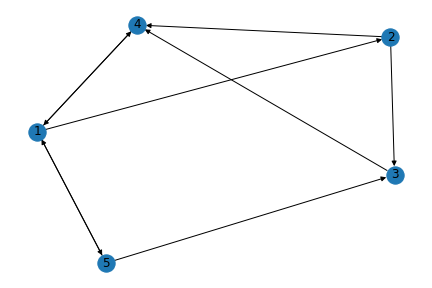
\includegraphics[scale=0.7]{images/redes-1-grafo-exemplo.png}
 \fautor
\end{figure}

A figura \ref{fig:redes1:grafo-exemplo} representa um grafo que pode ser representado pela matriz:

\begin{equation}
A = \begin{bmatrix}
0 & 1 & 0 & 1 & 1 \\
0 & 0 & 1 & 1 & 0 \\
0 & 0 & 0 & 1 & 0 \\
1 & 0 & 0 & 0 & 0 \\
1 & 0 & 1 & 0 & 0 \\
\end{bmatrix}
\end{equation}

outros conceitos usados na seção seguinte

\section{Métricas}

descricao das métricas usadas


\chapter{Base de Dados}
\label{chapter:base-de-dados}

Neste capítulo, serão descritos os conjuntos de dados utilizados neste trabalho, bem como os processos de extração e transformação envolvidos.

\section{Dados de Documentos Fiscais}
\label{section:base-de-dados:dados-de-documentos-fiscais}

Nesta seção, será apresentado o tratamento dos dados obtidos através da coleta de documentos fiscais.

\subsection{Aquisição}
\label{section:base-de-dados:dados-de-documentos-fiscais:aquisicao}

Como descrito na Seção~\ref{section:documentos-fiscais:arquivei}, os dados utilizados neste trabalho são obtidos através do armazém de dados da empresa parceira. Estes dados passam por um complexo processo de ingestão e tratamento descrito em detalhes no Apêndice~\ref{chapter:armazem-de-dados}.

A seleção dos dados foi feita usando o armazém de dados, através da linguagem \sigla{SQL}{\textit{Structured Query Language}}. Os critérios de seleção utilizados para obter os dados do armazém de dados foram:

\begin{itemize}
    \item Foram utilizados apenas dados de Notas Fiscais Eletrônicas, excluindo outros documentos fiscais
    \item Foram utilizados apenas documentos obtidos através do \textit{webservice} da Sefaz
    \item Foram utilizados apenas dados de documentos emitidos entre 01 de janeiro de 2019 e 31 de outubro de 2020
    \item Foram utilizados apenas documentos contendo a assinatura digital do emitente
    \item Foram utilizados apenas documentos contendo o protocolo de processamento do \textit{webservice} da Sefaz
    \item Foram utilizados apenas documentos cuja emissão foi autorizada pelo \textit{webservice} da Sefaz
    \item Foram utilizados apenas documentos referentes a transações cujo \sigla{CFOP}{Código Fiscal de Operações e Prestações} se refere às movimentações entre empresas envolvendo comercialização de mercadorias. Esses critérios são explicados em detalhes no Apêndice~\ref{chapter:cfop}
\end{itemize}

Os campos considerados são descritos no Quadro~\ref{quadro:campos-considerados-nfe}. Os tipos de dados e suas peculiaridades são descritos no Apêndice~\ref{chapter:tecnologias-utilizadas}.

\begin{quadro}[htb]
\caption{Campos de documentos fiscais considerados}
\label{quadro:campos-considerados-nfe}
\centering
\begin{tabular}{|l|l|l|}        \hline
\textbf{Nome do campo} & \textbf{Tipo de dado} & \textbf{Descrição}            \\ \hline
ID               & STRING       & Chave de acesso da NFe (anonimizado)         \\ \hline
dhEmi            & DATETIME     & Data e Hora de emissão do Documento Fiscal   \\ \hline
emit             & RECORD       & Identificação do Destinatário                \\
emit.CNPJ        & STRING       & Número do CNPJ do emitente (anonimizado)     \\ \hline
dest             & RECORD       & Identificação do Destinatário                \\
dest.CNPJ        & STRING       & Número do CNPJ do destinatário (anonimizado) \\ \hline
det              & ARRAY        & Dados dos detalhes da NF-e                   \\
det.prod         & RECORD       & Dados dos produtos e serviços da NF-e        \\
det.prod.\_nItem & INTEGER      & Número do item do NF                         \\
det.prod.VProd   & FLOAT        & Valor bruto do produto ou serviço            \\
det.prod.CFOP    & STRING       & CFOP                                         \\ \hline
\end{tabular}
\end{quadro}

Cada linha do conjunto de dados possui dados de uma transação entre duas empresas, identificada por uma chave de acesso única por transação, e que contém um ou mais produtos envolvidos com seus respectivos números de item, valor bruto, e CFOP.

Todos os dados obtidos a partir do armazém de dados foram anonimizados. Dados identificadores ou sensíveis foram removidos e reindexados de forma a manter o sigilo e privacidade de tais dados respeitando tanto a legislação atual quanto os contratos de prestação de serviços da empresa parceira.

\subsection{Pré-processamento}
\label{section:base-de-dados:dados-de-documentos-fiscais:preprocessamento}

Para cada documento foi criada uma nova coluna com o valor bruto agregado dos produtos transacionados, respeitando os critérios de CFOP e sendo eliminados os documentos de valor zero (o que é possível devido a inconsistências durante a emissão do documento).

Para remover eventuais problemas de completude nos dados, foram considerados apenas documentos de transações entre empresas recorrentes. Chamamos de \textbf{empresas recorrentes} aquelas que possuem pelo menos um documento na base de dados emitido para cada mês entre janeiro de 2019 e outubro de 2020.

Uma vez tratados os dados, estes foram agregados em três conjuntos adicionais de dados, agregados por:

\begin{itemize}
    \item \sigla{UF}{Unidade Federativa}
    \item Seção de CNAE
    \item CNAE
\end{itemize}

Cada um dos três conjuntos de dados agrega informações das transações efetuadas durante um mês, de janeiro de 2019 a outubro de 2020, sendo agregada a informação do valor total bruto dos produtos transacionados.

Uma nova coluna foi criada contendo a quantidade de transações mensal entre cada entidade. Foi considerado que cada NF-e documenta uma única transação independente da quantidade de produtos envolvida.

\section{Dados Abertos de Empresas Brasileiras}
\label{section:base-de-dados:dados-abertos}

Nesta seção, será apresentado o tratamento dos dados obtidos através da base de dados abertos da Receita Federal.

\subsection{Aquisição}
\label{section:base-de-dados:dados-abertos:aquisicao}

Além dos dados descritos na Seção~\ref{section:base-de-dados:dados-de-documentos-fiscais}, foram utilizados também dados coletados das bases de dados abertas sobre o Cadastro Nacional de Pessoas Jurídicas da Receita Federal \cite{receita:dados-publicos:cnpj}.

Tais dados são divulgados conforme previsto no Artigo 5º da Constituição Federal \cite{constituicao:1988}:

\begin{citacao}
Art. 5º Todos são iguais perante a lei, sem distinção de qualquer natureza, garantindo-se aos brasileiros e aos estrangeiros residentes no País a inviolabilidade do direito à vida, à liberdade, à igualdade, à segurança e à propriedade, nos termos seguintes:

...

XXXIII - todos têm direito a receber dos órgãos públicos informações de seu interesse particular, ou de interesse coletivo ou geral, que serão prestadas no prazo da lei, sob pena de responsabilidade, ressalvadas aquelas cujo sigilo seja imprescindível à segurança da sociedade e do Estado;

...
\end{citacao}

Regulado pela Lei de Acesso a Informação \cite{lei:12527:lei-de-acesso-a-informacao}:

\begin{citacao}
Art. 8º É dever dos órgãos e entidades públicas promover, independentemente de requerimentos, a divulgação em local de fácil acesso, no âmbito de suas competências, de informações de interesse coletivo ou geral por eles produzidas ou custodiadas.

...

§ 3º Os sítios de que trata o § 2º deverão, na forma de regulamento, atender, entre outros, aos seguintes requisitos:

...

III - possibilitar o acesso automatizado por sistemas externos em formatos abertos, estruturados e legíveis por máquina;

...
\end{citacao}

Esses dados são também tratados e estão disponíveis no armazém de dados da empresa parceira através do processo descrito no Apêndice~\ref{chapter:armazem-de-dados}. De lá foram coletadas as seguintes informações a partir da base de dados completa, cujos campos são descritos no Quadro~\ref{quadro:campos-considerados-nfe}.

\begin{quadro}[htb]
\caption{Campos do Cadastro Nacional de Pessoas Jurídicas considerados}
\label{quadro:campos-considerados-cnpj}
\centering
\begin{tabularx}{\textwidth}{|l|l|X|} \hline
\textbf{Nome do campo} & \textbf{Tipo de dado} & \textbf{Descrição}                   \\ \hline
CNPJ                & STRING       & Número de Inscrição no CNPJ                      \\ \hline
SituacaoCadastral   & STRING       & Código da Situação Cadastral                     \\ \hline
DataInicioAtividade & STRING       & Data de Início da Atividade                      \\ \hline
CnaeFiscal          & STRING       & Código da Atividade Econômica                    \\ \hline
UF                  & STRING       & Sigla da UF em que se encontra o estabelecimento \\ \hline
Municipio           & STRING       & Código do município de jurisdição onde se encontra o estabelecimento \\ \hline
Porte               & STRING       & Código do porte da empresa                       \\ \hline
OpcaoSimples        & STRING       & Indicador da existência da opção pelo simples    \\ \hline
OpcaoMei            & STRING       & Indicador da existência da opção pelo MEI        \\ \hline
\end{tabularx}
\end{quadro}

Através do número de inscrição das empresas foi possível cruzar os dados obtidos nesta base de dados com a base de dados descrita na Seção~\ref{section:base-de-dados:dados-de-documentos-fiscais}, o que foi feito antes de todo o processo de anonimização citado nessa seção.

\section{Análise Descritiva da Base de Dados}
\label{section:base-de-dados:analise-descritiva}

Nesta seção, será apresentada uma análise descritiva dos dados utilizados neste trabalho, descrevendo os dados coletados de documentos fiscais e comparando sua abrangência com os dados obtidos da base de dados aberta da Receita Federal.

\subsection{Abrangência territorial}
\label{section:base-de-dados:analise-descritiva:abrangencia-territorial}

Nesta subseção, será apresentada a análise descritiva do ponto de vista territorial. Será descrita a participação das empresas citadas na base de dados em relação aos totais de cada divisão territorial brasileira a partir dos dados descritos na Seção~\ref{section:base-de-dados:dados-abertos}.

O IBGE criou a \sigla{DTB}{Divisão Territorial Brasileira}, uma codificação hierárquica de sete dígitos do território brasileiro onde:

\begin{itemize}
    \item O primeiro dígito indica a região
    \item O segundo dígito indica a UF
    \item O terceiro e quarto dígito indicam a mesorregião
    \item O sexto dígito indica a microrregião
    \item O sétimo dígito indica o município
\end{itemize}

O Quadro~\ref{quadro:tabela-codigo-regiao} descreve as regiões brasileiras segundo esta divisão, que foi usada no estudo de abrangência territorial dos dados.

\begin{quadro}[htb]
\caption{Códigos de Região segundo DTB}
\label{quadro:tabela-codigo-regiao}
\centering
\begin{tabular}{|l|l|l|}        \hline
\textbf{Código da Região} & \textbf{Região} & \textbf{Unidade Federativa } \\ \hline
\multirow{7}{*}{1} & \multirow{7}{*}{Região Norte}        & Acre\\
  &                                      & Amapá\\
  &                                      & Amazonas\\
  &                                      & Pará\\
  &                                      & Rondônia\\
  &                                      & Roraima\\
  &                                      & Tocantins\\ \hline
\multirow{9}{*}{2} & \multirow{9}{*}{Região Nordeste}     & Alagoas\\
  &                                      & Bahia\\
  &                                      & Ceará\\
  &                                      & Maranhão\\
  &                                      & Paraíba\\
  &                                      & Pernambuco\\
  &                                      & Piauí\\
  &                                      & Rio Grande do Norte\\
  &                                      & Sergipe\\\hline
\multirow{4}{*}{3} & \multirow{4}{*}{Região Centro-Oeste} & Distrito Federal\\
  &                                      & Goiás\\
  &                                      & Mato Grosso\\
  &                                      & Mato Grosso do Sul\\ \hline
\multirow{4}{*}{4} & \multirow{4}{*}{Região Sudeste}      & Espírito Santo\\
  &                                      & Minas Gerais\\
  &                                      & São Paulo\\
  &                                      & Rio de Janeiro\\ \hline
\multirow{3}{*}{5} & \multirow{3}{*}{Região Sul}          & Paraná\\
  &                                      & Rio Grande do Sul\\
  &                                      & Santa Catarina\\ \hline
\end{tabular}
\end{quadro}

Na Figura~\ref{fig:base-de-dados:descritiva-1.1-presenca-por-regiao-1.1} é descrito o percentual do total das empresas de cada região que foi encontrada na base de dados deste trabalho. Os dados são descritos em detalhe na Tabela~\ref{tab:participacao-por-regiao}. A Figura~\ref{fig:base-de-dados:descritiva-1.2-qtde-por-regiao} descreve as quantidades de empresas presentes na base de dados em relação ao total de cada região brasileira.

Com esses dados é possível observar que a participação em termos regionais é significativa e que há um razoável balanceamento regional, com uma participação regional que varia entre 7 e 10\%, mas sem um grande viés para uma das regiões. A quantidade de empresas da Região 4 é significativamente maior em comparação à outras regiões, mas reflete proporcionalmente a realidade se verificarmos os valores percentuais.

\begin{figure}[htb]
    \centering
    \caption{Participação por região das empresas presentes na base de dados}
    \label{fig:base-de-dados:descritiva-1-presenca-por-regiao} 
    \begin{subfigure}[b]{0.45\textwidth} 
        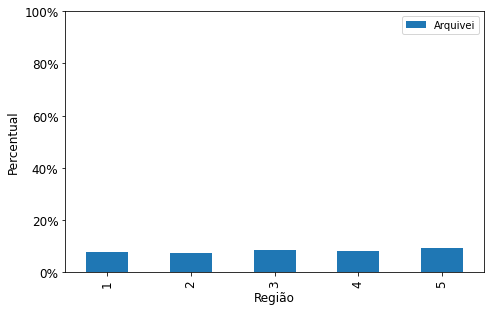
\includegraphics[scale=0.45]{images/base-de-dados-1.1-presenca-por-regiao.png}
        \caption{Percentual das empresas de cada região brasileira presente na base de dados}
        \label{fig:base-de-dados:descritiva-1.1-presenca-por-regiao-1.1}
    \end{subfigure} ~ \quad
    \begin{subfigure}[b]{0.45\textwidth}
        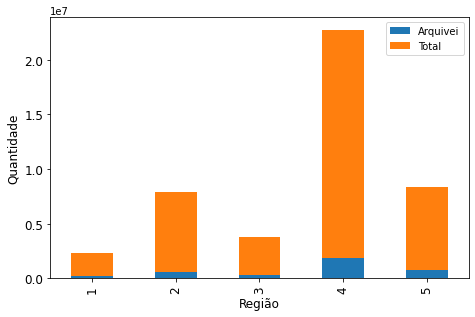
\includegraphics[scale=0.45]{images/base-de-dados-1.2-qtde-por-regiao.png}
        \caption{Quantidade de empresas de cada região brasileira presente na base de dados relativa ao total}
        \label{fig:base-de-dados:descritiva-1.2-qtde-por-regiao}
    \end{subfigure}
    \fdadospesquisa
\end{figure}

\begin{table}[htb]
\centering
\caption{Percentual das empresas presentes na base de dados por Região}
\label{tab:participacao-por-regiao}
\begin{tabular}{lr}
\toprule
Região & Participação \\
\midrule
1      &    7.88\% \\
2      &    7.26\% \\
3      &    8.41\% \\
4      &    8.00\% \\
5      &    9.39\% \\
\bottomrule
\end{tabular}
\fdadospesquisa
\end{table}

A seguir, repetimos a análise agora para as Unidades Federativas do Brasil, ilustrada em participação percentual na Figura~\ref{fig:base-de-dados:descritiva-2.1-presenca-por-uf} e na Tabela~\ref{tab:participacao-por-uf}, e em quantidades em relação à quantidade total de cada UF na Figura~\ref{fig:base-de-dados:descritiva-2.2-qtde-por-uf}.

\begin{figure}[htb]
    \centering
    \caption{Participação por UF das empresas presentes na base de dados}
    \label{fig:base-de-dados:descritiva-2-presenca-por-uf}
    \begin{subfigure}[b]{1.00\textwidth} 
        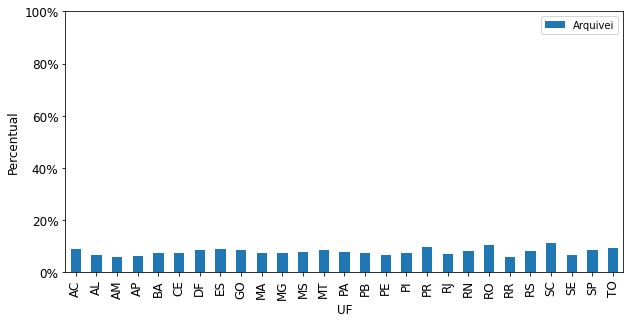
\includegraphics[scale=0.7]{images/base-de-dados-2.1-presenca-por-uf.png}
        \caption{Percentual das empresas das cada UF presente na base de dados}
        \label{fig:base-de-dados:descritiva-2.1-presenca-por-uf}
    \end{subfigure} ~ \\
    \begin{subfigure}[b]{1.00\textwidth}
        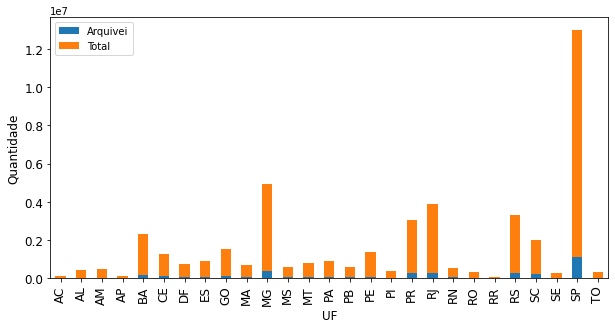
\includegraphics[scale=0.7]{images/base-de-dados-2.2-qtde-por-uf.png}
        \caption{Quantidade de empresas de cada UF presente na base de dados relativa ao total}
        \label{fig:base-de-dados:descritiva-2.2-qtde-por-uf}
    \end{subfigure}
    \fdadospesquisa
\end{figure}

\begin{table}[htb]
\centering
\caption{Percentual das empresas presentes na base de dados por UF}
\label{tab:participacao-por-uf}
\begin{subtable}[h]{0.45\textwidth}
    \centering
    \begin{tabular}{l|r}
        \toprule
        UF & Participação \\
        \midrule
        AC &    8.93\% \\
        AL &    6.75\% \\
        AM &    5.76\% \\
        AP &    6.25\% \\
        BA &    7.34\% \\
        CE &    7.46\% \\
        DF &    8.48\% \\
        ES &    8.95\% \\
        GO &    8.64\% \\
        MA &    7.56\% \\
        MG &    7.41\% \\
        MS &    7.67\% \\
        MT &    8.44\% \\
        PA &    7.91\% \\
        \bottomrule
    \end{tabular}
\end{subtable}
\begin{subtable}[h]{0.45\textwidth}
    \centering
    \begin{tabular}{l|r}
        \toprule
        UF & Participação \\
        \midrule
        PB &    7.43\% \\
        PE &    6.68\% \\
        PI &    7.49\% \\
        PR &    9.58\% \\
        RJ &    7.14\% \\
        RN &    8.03\% \\
        RO &    0.34\% \\
        RR &    6.04\% \\
        RS &    8.16\% \\
        SC &    1.15\% \\
        SE &    6.45\% \\
        SP &    8.41\% \\
        TO &    9.13\% \\
        \bottomrule
    \end{tabular}
\end{subtable}
\fdadospesquisa
\end{table}

Da mesma forma, é possível observar que a participação por unidade federativa é significativa e que embora haja um desbalanceamento um pouco maior, com uma participação por UF que varia entre 6 e 12\%, também não há um grande viés percentual para uma das UFs, refletindo razoavelmente a realidade.

Por fim, a Figura~\ref{fig:base-de-dados:descritiva-3.1-presenca-por-mun} mostra um histograma relacionando o percentual do total de empresas presentes na base de dados em relação aos municípios brasileiros. A Tabela~\ref{tab:participacao-por-mun} mostra algumas métricas sobre esta análise por municípios, mostrando que existe participação em todos os municípios brasileiros com uma média e mediana próximos de 7.5\% e pico de 21\%.

\begin{figure}[htb]
    \centering
    \caption{Histograma do percentual das empresas de cada município brasileiro presente na base de dados}
    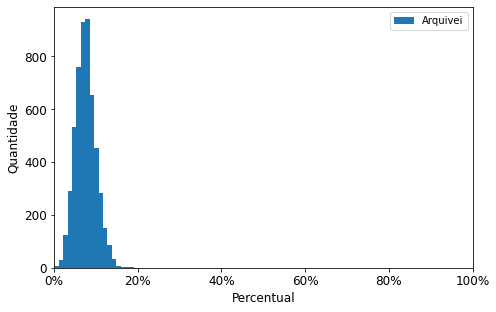
\includegraphics[scale=0.7]{images/base-de-dados-3.1-presenca-por-mun.png}
    \label{fig:base-de-dados:descritiva-3.1-presenca-por-mun}
    \fdadospesquisa
\end{figure}

\begin{table}[htb]
\centering
\caption{Métricas sobre o percentual das empresas presentes na base de dados por município}
\label{tab:participacao-por-mun}
\begin{tabular}{lr}
\toprule
Métrica & Valor \\
\midrule
Média         &    7.522\% \\
Desvio Padrão &    2.462\% \\
Mínimo        &    0.002\% \\
25º percentil &    5.834\% \\
50º percentil &    7.419\% \\
75º percentil &    9.065\% \\
Máximo        &   21.230\% \\
\bottomrule
\end{tabular}
\fdadospesquisa
\end{table}

Assim, pode-se observar uma forte participação territorial dos dados tanto observando do ponto de vista regional como também estadual e municipal, estando presentes nas mais diversas realidades brasileiras.

\subsection{Abrangência econômica}
\label{section:base-de-dados:analise-descritiva:abrangencia-economica}

Os dados descritos na Seção~\ref{section:base-de-dados:dados-abertos} apresentam uma série de informações e classificações das empresas que podem ser utilizadas para ter uma melhor noção do porte e dos tipos de empresas envolvidas. Nesta subseção, será apresentada a análise descritiva do ponto de vista econômico em relação aos totais coletados daquela base.

A primeira classificação que vamos considerar para esta análise é o \textbf{porte} de uma empresa. Regulada pela Lei nº 5172/1966 ~\cite{lei:5172:codigo-tributario}, que em seu Artigo 3º define:

\begin{citacao}
Art. 3º Para os efeitos desta Lei Complementar, consideram-se \textbf{microempresas} ou \textbf{empresas de pequeno porte}, a sociedade empresária, a sociedade simples, a empresa individual de responsabilidade limitada e o empresário a que se refere o art. 966 da Lei no 10.406, de 10 de janeiro de 2002 (Código Civil), devidamente registrados no Registro de Empresas Mercantis ou no Registro Civil de Pessoas Jurídicas, conforme o caso, desde que:

I - no caso da microempresa, aufira, em cada ano-calendário, receita bruta igual ou inferior a R\$ 360.000,00 (trezentos e sessenta mil reais); e

II - no caso de empresa de pequeno porte, aufira, em cada ano-calendário, receita bruta superior a R\$ 360.000,00 (trezentos e sessenta mil reais) e igual ou inferior a R\$ 4.800.000,00 (quatro milhões e oitocentos mil reais).

§ 1º  Considera-se receita bruta, para fins do disposto no caput deste artigo, o produto da venda de bens e serviços nas operações de conta própria, o preço dos serviços prestados e o resultado nas operações em conta alheia, não incluídas as vendas canceladas e os descontos incondicionais concedidos.

(...)
\end{citacao}

As empresas declaram seu porte no momento da sua inscrição no Cadastro Nacional de Pessoas Jurídicas, e esta declaração é revisada pela Receita Federal a partir de suas declarações fiscais anuais. Empresas cuja receita bruta não se enquadra nas categorias \sigla{ME}{Microempresa} e \sigla{EPP}{Empresa de Pequeno Porte} são enquadradas na categoria \textbf{Demais}. Em alguns casos específicos, as empresas não declaram sua receita bruta no ato da inscrição no cadastro, em sua maioria empresas estrangeiras presentes no cadastro, essas são enquadradas na categoria \textbf{Não Informado}.

A partir dos dados das Figuras~\ref{fig:base-de-dados:descritiva-4.1-presenca-por-porte} e~\ref{fig:base-de-dados:descritiva-4.2-qtde-por-porte} é possível verificar a participação das empresas presentes na base de dados em relação aos totais. A Tabela~\ref{tab:participacao-por-porte} descreve os valores em detalhes.

\begin{figure}[htb]
    \centering
    \caption{Participação por porte das empresas presentes na base de dados}
    \label{fig:base-de-dados:descritiva-4-presenca-por-porte}
    \begin{subfigure}[b]{0.45\textwidth} 
        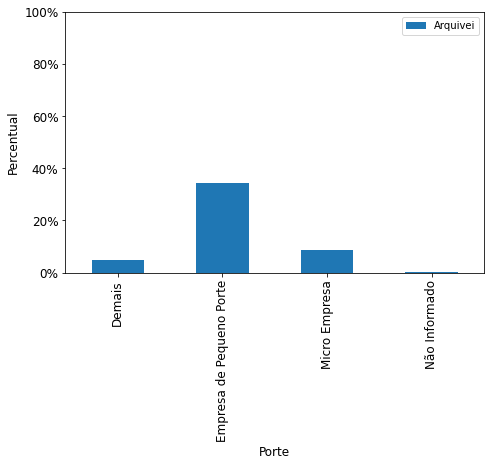
\includegraphics[scale=0.45]{images/base-de-dados-4.1-presenca-por-porte.png}
        \caption{Percentual das empresas presente na base de dados categorizadas por porte}
        \label{fig:base-de-dados:descritiva-4.1-presenca-por-porte}
    \end{subfigure} ~ \quad
    \begin{subfigure}[b]{0.45\textwidth}
        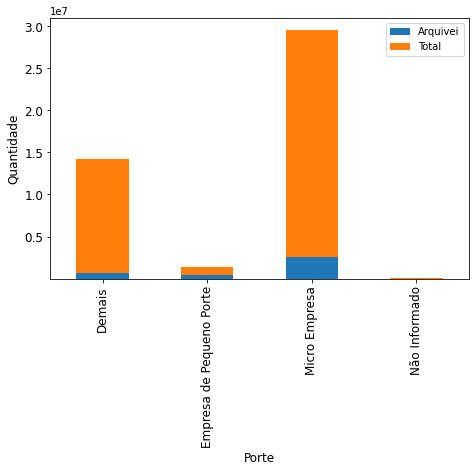
\includegraphics[scale=0.45]{images/base-de-dados-4.2-qtde-por-porte.png}
        \caption{Quantidade de empresas categorizadas por porte presente na base de dados relativa ao total}
        \label{fig:base-de-dados:descritiva-4.2-qtde-por-porte}
    \end{subfigure}
    \fdadospesquisa
\end{figure}

\begin{table}[htb]
\centering
\caption{Métricas sobre o percentual das empresas presentes na base de dados por porte}
\label{tab:participacao-por-porte}
\begin{tabular}{lr}
\toprule
Porte & Participação \\
\midrule
Demais                   &    4.76\% \\
Empresa de Pequeno Porte &    34.46\% \\
Micro Empresa            &    8.59\% \\
Não Informado            &    0.05\% \\
\bottomrule
\end{tabular}
\fdadospesquisa
\end{table}

É possível observar que há uma participação significativa desproporcional maior de EPPs nas empresas presentes da base de dados em relação à base de comparação. A participação é significativa também nos segmentos de Micro Empresas e Demais. Dentre as empresas que não informaram o porte a participação é proporcionalmente bastante baixa e suas quantidades totais na base de comparação são também muito pequenas.

A legislação brasileira define também a figura do \sigla{MEI}{Microempreendedor Individual} através do Código Civil Brasileiro \cite{lei:10406:lei-codigo-civil} que define a figura do empresário como:

\begin{citacao}
Art. 966. Considera-se empresário quem exerce profissionalmente atividade econômica organizada para a produção ou a circulação de bens ou de serviços.

Parágrafo único. Não se considera empresário quem exerce profissão intelectual, de natureza científica, literária ou artística, ainda com o concurso de auxiliares ou colaboradores, salvo se o exercício da profissão constituir elemento de empresa.
\end{citacao}

E da Lei nº 128/2008 \cite{lei:128:lei-mei} que estende essa definição para a figura do MEI:

\begin{citacao}
Art. 18-A.  O \textbf{Microempreendedor Individual - MEI} poderá optar pelo recolhimento dos impostos e contribuições abrangidos pelo Simples Nacional em valores fixos mensais, independentemente da receita bruta por ele auferida no mês, na forma prevista neste artigo.

§ 1o  Para os efeitos desta Lei, considera-se MEI o empresário individual a que se refere o art. 966 da Lei no 10.406, de 10 de janeiro de 2002 – Código Civil, que tenha auferido receita bruta, no ano-calendário anterior, de até R\$ 36.000,00 (trinta e seis mil reais), optante pelo Simples Nacional e que não esteja impedido de optar pela sistemática prevista neste artigo.  

§ 2o  No caso de início de atividades, o limite de que trata o § 1o deste artigo será de R\$ 3.000,00 (três mil reais) multiplicados pelo número de meses compreendido entre o início da atividade e o final do respectivo ano-calendário, consideradas as frações de meses como um mês inteiro.  
\end{citacao}

Empresários que optam pelo regime MEI tem uma série de facilidades fiscais que visam incentivar pequenos empresários, o que pode ser um fator importante para a sobrevivência do mesmo durante uma crise.

A partir dos dados sobre a participação por porte e da Opção pelo MEI, podemos verificar qual o percentual de participação nesta faixa econômica. Nesta análise, foram consideradas apenas as empresas que já declaram ter porte de Micro Empresa, um requisito devido à receita bruta máxima prevista na legislação, e então verificamos quais os percentuais presentes na base de dados.

A Figura~\ref{fig:base-de-dados:descritiva-5.1-presenca-por-mei} e~\ref{fig:base-de-dados:descritiva-5.2-qtde-por-mei}, cujos dados são detalhados na Tabela~\ref{tab:participacao-por-mei} mostram os dados de participação em relação à Opção pelo MEI. A microempresa tem a opção de optar ou não por este enquadramento no momento de sua abertura, mas existem casos em que não foi feita a opção, seja por omissão no momento do cadastro ou por ser anterior à lei que define o MEI. Casos onde não foi feita a opção são descritos nos dados como \textbf{Outros}.

É possível observar que nos dados coletados da empresa parceira existe algum viés para microempreendedores que não optam pelo MEI, seja explicitamente ou devido a outros fatores.

\begin{figure}[htb]
    \centering
    \caption{Participação por opção pelo MEI das empresas presentes na base de dados}
    \label{fig:base-de-dados:descritiva-5-qtde-por-mei}
    \begin{subfigure}[b]{0.45\textwidth} 
        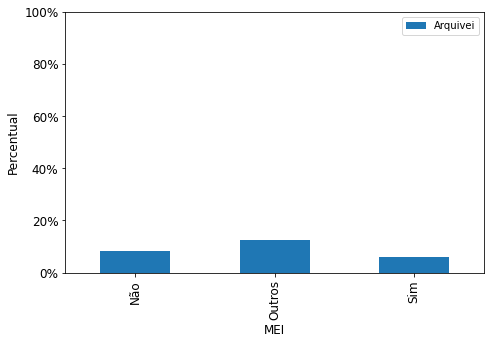
\includegraphics[scale=0.45]{images/base-de-dados-5.1-presenca-por-mei.png}
        \caption{Percentual das empresas presente na base de dados categorizadas pela opção por MEI}
        \label{fig:base-de-dados:descritiva-5.1-presenca-por-mei}
    \end{subfigure} ~ \quad
    \begin{subfigure}[b]{0.45\textwidth}
        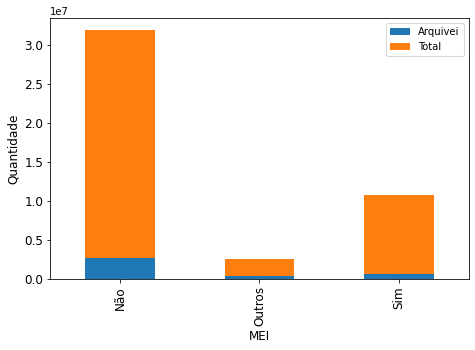
\includegraphics[scale=0.45]{images/base-de-dados-5.2-qtde-por-mei.png}
        \caption{Quantidade de empresas categorizadas pela opção por MEI presente na base de dados relativa ao total}
        \label{fig:base-de-dados:descritiva-5.2-qtde-por-mei}
    \end{subfigure}
    \fdadospesquisa
\end{figure}

\begin{table}[htb]
\centering
\caption{Métricas sobre o percentual das empresas presentes na base de dados pela opção pelo MEI}
\label{tab:participacao-por-mei}
\begin{tabular}{lr}
\toprule
Opção pelo MEI & Participação \\
\midrule
Não      &    10.20\% \\
Outros   &     7.03\% \\
Sim      &     5.98\% \\
\bottomrule
\end{tabular}
\fdadospesquisa
\end{table}

A Lei nº 123/2006 \cite{lei:123:lei-estatuto-mei-e-epp} institui o Simples Nacional, um regime tributário que facilita o recolhimentos de impostos para MEIs e EPPs. A base de dados abertos da Receita Federal também possui a informação da opção ou não pelo regime Simples Nacional. As empresas podem solicitar a exclusão do regime Simples Nacional mediante apresentação de ofício, ou em alguns casos previstos na lei onde a empresa deixa de cumprir alguns requisitos ou obrigações, nestes casos a empresa consta na base de dados como Excluído.

As Figuras~\ref{fig:base-de-dados:descritiva-6-presenca-por-simples-nacional} e~\ref{fig:base-de-dados:descritiva-6.2-qtde-por-simples-nacional}, detalhados na Tabela~\ref{tab:participacao-por-simples-nacional}, mostram a relação entre os dados presentes na base de dados em relação aos totais coletados da Receita Federal. É possível verificar que na base de dados é mais comum a presença de empresas optantes pelo regime Simples Nacional, e assim como em relação à opção ou não pelo MEI isso pode ser um fator de resiliência ou não à crises.

\begin{figure}[htb]
    \centering
    \caption{Participação por região das empresas presentes na base de dados}
    \label{fig:base-de-dados:descritiva-6-presenca-por-simples-nacional}
    \begin{subfigure}[b]{0.45\textwidth} 
        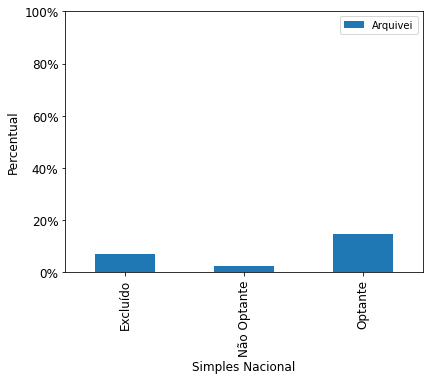
\includegraphics[scale=0.45]{images/base-de-dados-6.1-presenca-por-simples-nacional.png}
        \caption{Percentual das empresas presente na base de dados categorizadas pela opção pelo Simples Nacional}
        \label{fig:base-de-dados:descritiva-6.1-presenca-por-simples-nacional}
    \end{subfigure} ~ \quad
    \begin{subfigure}[b]{0.45\textwidth}
        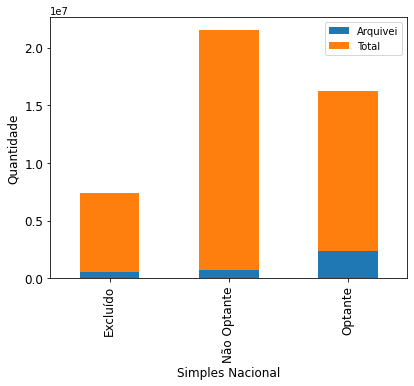
\includegraphics[scale=0.45]{images/base-de-dados-6.2-qtde-por-simples-nacional.png}
        \caption{Quantidade de empresas categorizadas pela opção pelo Simples Nacional presente na base de dados relativa ao total}
        \label{fig:base-de-dados:descritiva-6.2-qtde-por-simples-nacional}
    \end{subfigure}
    \fdadospesquisa
\end{figure}

\begin{table}[htb]
\centering
\caption{Métricas sobre o percentual das empresas presentes na base de dados pela Opção pelo Simples Nacional}
\label{tab:participacao-por-simples-nacional}
\begin{tabular}{lr}
\toprule
Opção pelo Simples Nacional & Participação \\
\midrule
Excluído     &    0.0693 \\
Não Optante  &    0.0229 \\
Optante      &    0.1450 \\
\bottomrule
\end{tabular}
\fdadospesquisa
\end{table}

\subsection{Abrangência setorial}

Nesta Seção, será feita a análise comparativa dos dados presentes na base de dados de documentos fiscais em relação aos dados abertos descritos na Seção~\ref{section:base-de-dados:dados-abertos} visando descrever a participação em relação aos setores econômicos da economia brasileira.

Como citado no Capítulo~\ref{chapter:documenos-fiscais}, através dos protocolos do ENAT foi feito o compromisso para a unificação do Cadastro Nacional de Atividades Econômicas (CNAE). Esse cadastro foi implementado então pela Resolução IBGE/CONCLA \sigla*{CONCLA}{Comissão Nacional de Classificação} nº 01 de 04 de setembro de 2006 \cite{resolucao-concla:01:cnae} e Resolução IBGE/CONCLA nº nº 02, de 15 de dezembro de 2006 \cite{resolucao-concla:02:cnae}. Como descrito no Art. 1º da Resolução nº 01, essa classificação é hierárquica:

\begin{citacao}
O PRESIDENTE DA COMISSÃO NACIONAL DE CLASSIFICAÇÃO –
CONCLA, no uso de suas atribuições, resolve:

Art. 1 o Aprovar e divulgar a estrutura completa da Classificação Nacional de Atividades Econômicas – CNAE – versão 2.0, organizada em cinco níveis hierárquicos: seções, divisões, grupos, classes e subclasses, sendo o detalhamento das subclasses destinado ao uso da Administração Pública Brasileira.

(...)
\end{citacao}

O anexo de tal resolução contém uma tabela com o detalhamento dessa classificação, posteriormente retificada.

As empresas informam o código de sua CNAE Fiscal no momento da sua inscrição no Cadastro Nacional de Pessoas Jurídicas, e este dado fica disponível para consulta pública através de sua base de dados aberta. São informadas também os códigos de suas CNAEs secundários referentes a atividades secundárias das empresas, estes não foram utilizados nesta análise.

O Quadro~\ref{quadro:denominacao-secao-cnae} descreve a que se refere cada seção segundo o IBGE/CONCLA.

\begin{quadro}[htb]
\caption{Denominação das Seções de CNAE}
\label{quadro:denominacao-secao-cnae}
\centering
\begin{tabularx}{\textwidth}{|l|l|X|}        \hline
\textbf{Seção} & \textbf{Faixa de Divisões} & \textbf{Denominação} \\ \hline
A & 01 a 03 & Agricultura, pecuária, produção florestal, pesca e aquicultura \\ \hline
B & 05 a 09 & Indústrias extrativas \\ \hline
C & 10 a 33 & Indústrias de transformação \\ \hline
D & 35      & Eletricidade e gás \\ \hline
E & 36 a 39 & Água, esgoto, atividades de gestão de resíduos e descontaminação \\ \hline
F & 41 a 43 & Construção \\ \hline
G & 45 a 47 & Comércio; Reparação de veículos automotores e motocicletas \\ \hline
H & 49 a 53 & Transporte, armazenagem e correio \\ \hline
I & 55 a 56 & Alojamento e alimentação \\ \hline
J & 58 a 63 & Informação e comunicação \\ \hline
K & 64 a 66 & Atividades financeiras, de seguros e serviços relacionados \\ \hline
L & 68      & Atividades imobiliárias \\ \hline
M & 69 a 75 & Atividades profissionais, científicas e técnicas \\ \hline
N & 77 a 82 & Atividades administrativas e serviços complementares \\ \hline
O & 84      & Administração pública, defesa e seguridade social \\ \hline
P & 85      & Educação \\ \hline
Q & 86 a 88 & Saúde humana e serviços sociais \\ \hline
R & 90 a 93 & Artes, cultura e serviços sociais \\ \hline
S & 94 a 96 & Outras atividades de serviços \\ \hline
T & 97      & Serviços Domésticos \\ \hline
U & 99      & Organismos internacionais e outras instituições extraterritoriais \\ \hline
\end{tabularx}
\end{quadro}

As Figuras~\ref{fig:base-de-dados:descritiva-7.1-presenca-por-secao} e \ref{fig:base-de-dados:descritiva-7.2-qtde-por-secao} descrevem a participação percentual por seção econômica e suas quantidades em relação aos totais. A Tabela~\ref{tab:participacao-por-secao} descreve a participação percentual em detalhes.

\begin{figure}[htb]
    \centering
    \caption{Participação por seção do CNAE das empresas presentes na base de dados}
    \label{fig:base-de-dados:descritiva-7-presenca-por-secao}
    \begin{subfigure}[b]{1.0\textwidth} 
        \centering
        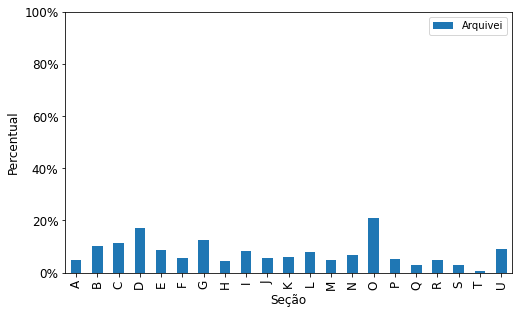
\includegraphics[scale=0.7]{images/base-de-dados-7.1-presenca-por-secao.png}
        \caption{Percentual das empresas presente na base de dados categorizadas pela seção do CNAE}
        \label{fig:base-de-dados:descritiva-7.1-presenca-por-secao}
    \end{subfigure} ~ \\
    \begin{subfigure}[b]{1.0\textwidth}
        \centering
        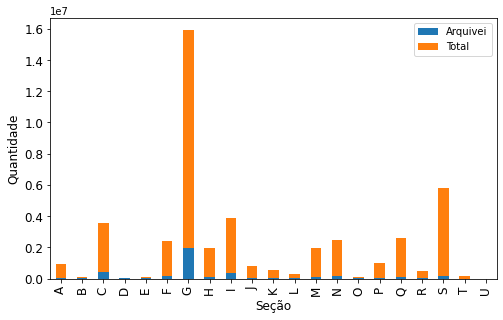
\includegraphics[scale=0.7]{images/base-de-dados-7.2-qtde-por-secao.png}
        \caption{Quantidade de empresas categorizadas seção do CNAE presente na base de dados relativa ao total}
        \label{fig:base-de-dados:descritiva-7.2-qtde-por-secao}
    \end{subfigure}
    \fdadospesquisa
\end{figure}

\begin{table}[htb]
\centering
\caption{Métricas sobre o percentual das empresas presentes na base de dados por Seção do CNAE}
\label{tab:participacao-por-secao}
\begin{subtable}[h]{0.45\textwidth}
    \centering
    \begin{tabular}{l|r}
        \toprule
        Seção & Participação \\
        \midrule
        A     &     4.74\% \\
        B     &    10.31\% \\
        C     &    11.30\% \\
        D     &    17.17\% \\
        E     &     8.69\% \\
        F     &     5.66\% \\
        G     &    12.34\% \\
        H     &     4.36\% \\
        I     &     8.40\% \\
        J     &     5.41\% \\
        K     &     5.91\% \\
        \bottomrule
    \end{tabular}
\end{subtable}
\begin{subtable}[h]{0.45\textwidth}
    \centering
    \begin{tabular}{l|r}
        \toprule
        Seção & Participação \\
        \midrule
        L     &     7.87\% \\
        M     &     4.71\% \\
        N     &     6.66\% \\
        O     &    20.72\% \\
        P     &     5.22\% \\
        Q     &     3.01\% \\
        R     &     4.75\% \\
        S     &     2.82\% \\
        T     &     0.71\% \\
        U     &     9.07\% \\
        \bottomrule
    \end{tabular}
\end{subtable}
\fdadospesquisa
\end{table}

Através destes dados é possível notar que existe uma participação significativa em praticamente todas as seções, com exceção da seção T, de serviços domésticos. Os dados também possuem razoável viés para alguns setores que possuem altos percentuais, particularmente D, G, e O, em oposição aos outros. A quantidade de empresas de cada seção também varia significativamente, particularmente a seção G que possui um número bastante alto de empresas, o que não necessariamente implica maior quantidade de documentos fiscais ou valor transacionado, análise que será feita posteriormente.

A Figura~\ref{fig:base-de-dados:descritiva-9.1-presenca-por-cnae} ilustra a participação percentual por CNAE, e a Tabela~\ref{tab:participacao-por-cnae} nos dá algumas métricas acerca da participação por CNAE. Dos 1342 CNAEs existentes na base de dados de comparação, 1327 são citados na base de dados de documentos fsicais (98.88\%), com uma média de cerca de 15\% de participação e desvio padrão de cerca de 12\%.

É possível observar então que que há uma grande abrangência setorial, uma vez que a base de dados possui exemples da grande maioria das seções, mas o histograma mostra que existe uma grande quantidade de CNAEs com baixo percentual de participação.

\begin{figure}[htb]
	\centering
    \caption{Histograma do percentual das empresas de cada CNAE presente na base de dados}
    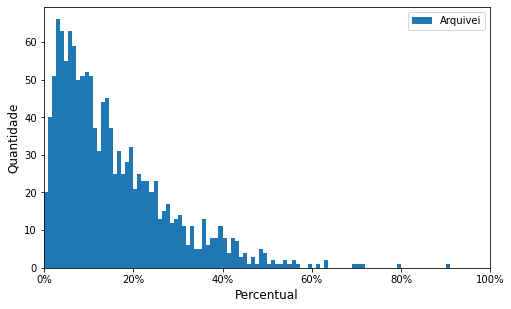
\includegraphics[scale=0.7]{images/base-de-dados-9.1-presenca-por-cnae.png}
    \label{fig:base-de-dados:descritiva-9.1-presenca-por-cnae}
    \fdadospesquisa
\end{figure}

\begin{table}[htb]
\centering
\caption{Métricas sobre o percentual das empresas presentes na base de dados por  CNAE}
\label{tab:participacao-por-cnae}
\begin{tabular}{lr}
\toprule
Métrica & Valor \\
\midrule
Média         &   15.371\% \\
Desvio Padrão &   12.452\% \\
Mínimo        &    0.004\% \\
25º percentil &    5.984\% \\
50º percentil &   12.056\% \\
75º percentil &   21.570\% \\
Máximo        &   90.909\% \\
\bottomrule
\end{tabular}
\fdadospesquisa
\end{table}

\section{Conclusões}

Neste capítulo, pudemos observar como os dados da base de dados de documentos fiscais utilizada neste trabalho se compara à base de dados aberta de empresas brasileiras. Do ponto de vista territorial, pudemos observar que há uma distribuição consideravelmente balanceada nos dados, não havendo grande preferência regional. Na análise de abrangência econômica, foi possível ver que existe certo viés para empresas de menor porte, com uma participação maior de MEs e EPPs em relação às Demais, o que reflete também a participação no Simples Nacional, uma tipificação típica de empresas de menor porte. Por fim, analisando a participação da base de dados em relação às seções da economia brasileira, pudemos observar que existe alguma variância entre as diversas seções de CNAE, e também entre todos os CNAEs.

Com isso, concluímos que os dados possuem algum viés e não são perfeitamente balanceados conforme a totalidade dos dados. Além disso, esta análise possui suas limitações, uma vez que não sabemos exatamente o volume de documentos nem de valores transacionados para cada tipo de empresa. O objetivo dessa análise foi tornar mais explícito a perspectiva que os dados apresentam acerca da totalidade dos dados da economia brasileira. Sob essa perspectiva faremos às análises seguintes, que são aplicadas sobre uma amostra dos dados totais, que pudemos ver que é significativa e razoavelmente balanceada segundo as segmentações que utilizamos.


\chapter{Impacto Econômico da Pandemia}
\label{chapter:impacto-economico}

Neste seção, será descrito o possível impacto econômico da Pandemia de COVID-19, contextualizada na Seção~\ref{introducao:pandemia}, verificando mensalmente se o volume transacionado foi próximo ou não no volume esperado.

\section{Cenário geral}
\label{section:impacto:cenario-geral}

Nessa seção, descrevemos os dados da base totalizados mensalmente de forma agregada.

\begin{figure}[htb]
	\centering
    \caption{Valor total transacionado por mês no período analisado}
    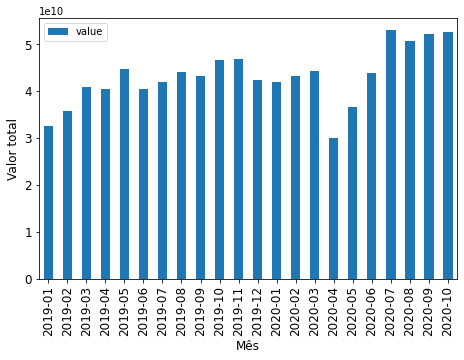
\includegraphics[scale=0.7]{images/base-de-dados-18.1-valor-mensal-total.png}
    \label{fig:pandemia:base-de-dados-18.1-valor-mensal-total}
    \fdadospesquisa
\end{figure}

\begin{figure}[htb]
	\centering
    \caption{Comparação do valor total transacionado por mês entre 2019 e 2020 (Parte 4)}
    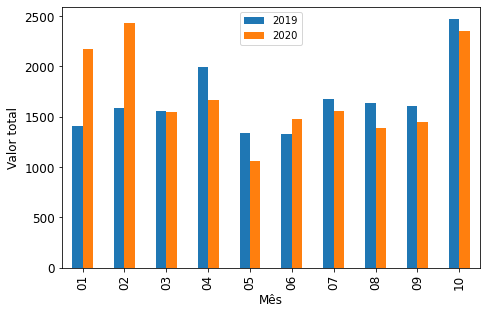
\includegraphics[scale=0.7]{images/base-de-dados-19.1-comparacao-valor-mensal-total.png}
    \label{fig:pandemia:base-de-dados-19.1-comparacao-valor-mensal-total}
    \fdadospesquisa
\end{figure}

A Figura~\ref{fig:pandemia:base-de-dados-18.1-valor-mensal-total} mostra o valor total transacionado em cada mês entre janeiro de 2019 e outubro de 2020, onde é visível um menor valor transacionado principalmente em abril e maio de 2020.

\begin{table}[htb]
\centering
\caption{Variação entre o valor transacionado para cada mês em 2020 em relação a 2019}
\label{tab:comparacao-valor-mensal-total}
\begin{tabular}{lr}
\toprule
Mês & Variação \\
\midrule
Janeiro &   25.49\% \\
Fevereiro & 14.58\% \\
Março &     12.71\% \\
Abril &    -12.24\% \\
Maio &     -11.24\% \\
Junho &      9.20\% \\
Julho &     11.64\% \\
Agosto &     7.52\% \\
Setembro &  17.02\% \\
Outubro &    3.33\% \\
\bottomrule
\end{tabular}
\fdadospesquisa
\end{table}

A Figura~\ref{fig:pandemia:base-de-dados-19.1-comparacao-valor-mensal-total} mostra uma comparação dos valores mensais transacionados em 2020 em relação aos valores mensais de 2019. Verifica-se então que os meses de abril e maio tiveram um valor total transacionado menor no ano de 2020, cuja variação por UF está descritos em detalhes na Tabela~\ref{tab:comparacao-valor-mensal-total}.

Como descrito na Seção~\ref{introducao:pandemia}, os meses de março e abril marcam exatamente o início do isolamento e das quarentenas no Brasil, e a aparentemente o impacto econômico nesses momentos foi mais importante.

Aplicando uma regressão linear a partir dos dados entre janeiro de 2019 e fevereiro de 2020 é possível obter uma da previsão de valor transacionado para os meses seguintes e então comparar com o valor obtido nos meses seguintes. Uma regressão linear não necessariamente é a melhor forma de prever o valor a ser transacionado para determinado mês, dados que os dados podem ter sazonalidades, porém se observarmos os dados da Figura~\ref{fig:pandemia:base-de-dados-18.1-valor-mensal-total}, podemos verificar uma tendência de crescimento linear mês a mês para os meses do ano de 2019. Isso não necessariamente ocorre porque houve um aumento real de transações das empresas envolvidas, mas porque a base de dados da empresa parceira tem crescido expressivamente mês a mês, com isso mesmo considerando o critério de recorrência, citado na seção~\ref{section:base-de-dados:dados-de-documentos-fiscais:preprocessamento}, a base de dados passa a receber mais dados de determinadas empresas, notoriamente aquelas que não são clientes da empresa parceira.

A Figura~\ref{fig:pandemia:base-de-dados-18.2-valor-total-vs-previsao} mostra os valores obtidos em relação aos valores previstos a partir da regressão linear aplicada sobre os dados, cuja variação é detalhada na na Tabela~\ref{tab:pandemia:valor-total-vs-previsao}.

\begin{figure}[htb]
	\centering
    \caption{Valor total transacionado por mês comparado com a previsão para o período analisado}
    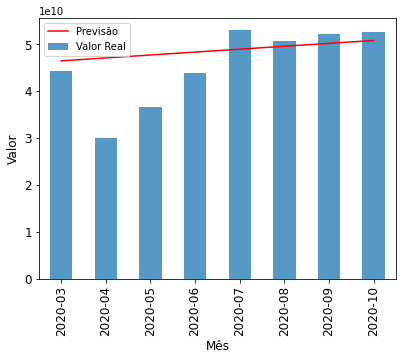
\includegraphics[scale=0.7]{images/base-de-dados-18.2-valor-total-vs-previsao.png}
    \label{fig:pandemia:base-de-dados-18.2-valor-total-vs-previsao}
    \fdadospesquisa
\end{figure}

\begin{table}[htb]
\centering
\caption{Variação entre o valor transacionado para cada mês em relação ao previsto após o início da pandemia}
\label{tab:pandemia:valor-total-vs-previsao}
\begin{tabular}{lr}
\toprule
Mês & Variação \\
\midrule
Março &     -4.46\% \\
Abril &    -36.22\% \\
Maio &     -23.11\% \\
Junho &     -9.15\% \\
Julho &      8.28\% \\
Agosto &     2.09\% \\
Setembro &   4.18\% \\
Outubro &    3.46\% \\ \hline
\textbf{Total} & -6.58\% \\
\bottomrule
\end{tabular}
\fdadospesquisa
\end{table}

A partir desses dados, é possível verificar que no período entre março e junho de 2020 o valor transacionado total foi menor que o previsto, verificando uma retomada posterior. Notoriamente, no mês de abril houve uma diferença de cerca de 36\% entre o valor previsto e o valor real. Dada essa leitura, vamos considerar posteriormente para efeitos de comparação que o segundo trimestre de 2020 foi o mais afetado economicamente pela pandemia, mesmo que no mês de março haja também impacto não o consideraremos pois as medidas de isolamento e distanciamento foram aplicadas apenas ao fim deste mês e o impacto não foi suficiente para alterar significativamente os totais do primeiro trimestre de 2020.

A partir de julho de 2020, o valor real transacionado foi maior que o valor previsto para esses meses. Isso pode indicar um menor impacto da pandemia para esses meses, e podemos observar na seção~\ref{introducao:pandemia} a partir da análise do índice de isolamento social que o isolamento social apesar de uma alta inicial em março e abril de 2020, começou a regredir a partir de julho de 2020, se mantendo estável após isso. Com isso, os níveis de consumo e produção possivelmente foram impactados positivamente com uma retomada, uma hipótese que ainda precisa ser mais lapidada uma vez que estamos analisando um período ainda limitado.

\section{Cenário regional}
\label{section:impacto:cenario-regional}

Nesta seção, descrevemos o impacto econômico da pandemia do ponto de vista regional. Usamos aqui a definição de região utilizada na seção~\ref{section:base-de-dados:analise-descritiva:abrangencia-territorial}. A Figura~\ref{fig:pandemia:base-de-dados-11.1-valor-total-por-regiao} mostra o valor total transacionado por região entre janeiro de 2019 e outubro de 2020 na base de dados utilizada neste trabalho.

\begin{figure}[htb]
	\centering
    \caption{Valor total transacionado por região no período analisado}
    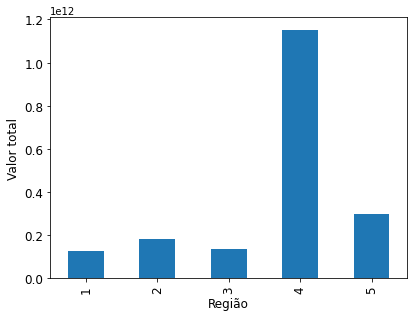
\includegraphics[scale=0.7]{images/base-de-dados-11.1-valor-total-por-regiao.png}
    \label{fig:pandemia:base-de-dados-11.1-valor-total-por-regiao}
    \fdadospesquisa
\end{figure}

A região 4 (sudeste) possui um valor transacionado muito maior em comparação às outras regiões. Segundo comparação feita na seção~\ref{section:base-de-dados:analise-descritiva:abrangencia-territorial}, não há uma preferência territorial clara para empresas da região sudeste possuindo um percentual de participação semelhante à de outras regiões. Esta região é conhecida por sua alta participação no cenário econômico brasileiro.

Na Figura~\ref{fig:pandemia:base-de-dados-21.1-valor-trimestral-por-regiao} é feita uma comparação trimestral entre o valor transacionado em cada um dos três primeiros trimestres de 2020 para cada região.

\begin{figure}[htb]
	\centering
    \caption{Valor trimestral transacionado por região no período analisado}
    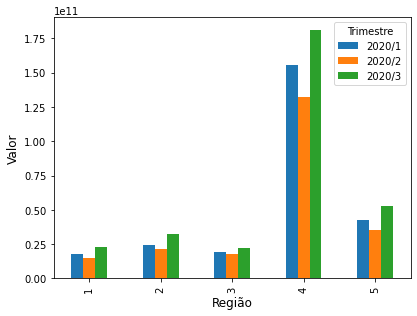
\includegraphics[scale=0.7]{images/base-de-dados-21.1-valor-trimestral-por-regiao.png}
    \label{fig:pandemia:base-de-dados-21.1-valor-trimestral-por-regiao}
    \fdadospesquisa
\end{figure}

Pode-se observar que todas as regiões tiveram um valor transacionado menor no segundo trimestre de 2020 em comparação aos outros dois trimestres analisados, o que indica um impacto econômico devido à crise causada pela pandemia, uma vez que os dados possuem uma tendência de crescimento no valor total transacionado, como argumentamos na seção~\ref{section:impacto:cenario-geral}.

A Tabela~\ref{tab:pandemia:variacao-por-regiao} descreve a diferença entre os valores previstos a partir de uma regressão linear aplicada sobre os dados de janeiro de 2019 a fevereiro de 2020 e àqueles obtidos para cada região entre março e outubro de 2020, da mesma forma como descrito na seção~\ref{section:impacto:cenario-geral}. Também é apresentada na mesma tabela a variação entre o valor total previto e obtido entre os meses de março a outubro de 2020.

\begin{table}[htb]
\centering
\caption{Diferença entre valores transacionados previstos e obtidos por região no período da pandemia}
\label{tab:pandemia:variacao-por-regiao}
\begin{subtable}[h]{\textwidth}
    \centering
    \begin{tabular}{c|r|r|r|r|r|r|r|r}
        \toprule
        \textbf{Região} & Março & Abril & Maio & Junho & Julho & Agosto & Setembro & Outubro \\
        \midrule
        \textbf{1} & -13.4\% & -48.8\% & -26.1\% &  -9.9\% &  8.9\% &  1.6\% &  0.7\% &  6.4\% \\
        \textbf{2} &  -9.2\% & -39.6\% & -22.3\% &  -5.3\% & 15.2\% & 10.1\% & 12.9\% & 18.9\% \\
        \textbf{3} &   8.2\% & -27.7\% & -10.7\% &   3.5\% &  9.6\% &  6.5\% &  8.4\% &  1.9\% \\
        \textbf{4} &  -3.0\% & -34.9\% & -23.8\% & -10.2\% &  3.0\% &  1.5\% &  3.4\% &  2.5\% \\
        \textbf{5} &  -8.5\% & -37.3\% & -24.9\% & -12.6\% & 22.5\% & -2.3\% &  1.6\% & -2.9\% \\
        \bottomrule
    \end{tabular}
    \caption{Diferença entre valor mensal previsto e obtido}
\end{subtable} ~ \\
\begin{subtable}[h]{0.45\textwidth}
    \centering
    \begin{tabular}{l|r}
        \toprule
        Região & Variação total \\
        \midrule
        \textbf{1} & -9.4\% \\
        \textbf{2} & -1.9\% \\
        \textbf{3} &  0.1\% \\
        \textbf{4} & -7.5\% \\
        \textbf{5} & -7.7\% \\
        \bottomrule
    \end{tabular}
    \caption{Diferença entre valor total previsto e obtido}
\end{subtable}
\fdadospesquisa
\end{table}

Verfificamos novamente que os meses mais impactados foram aqueles relativos ao segundo trimestre de 2020, de abril a junho. A diferença para o mês de abril chegou a ser de cerca de 48\% para a região 1 (norte), o que representa um impacto bastante significativo. É possível observar também cerca resiliência da região 3 (centro-oeste), sendo que essa região não apontou impacto no mês de março e foi capaz de se recuperar mais rapidamente já apresentando resultados positivos para o mês de junho. Com exceção da região 3, todas as regiões tiveram uma diferença entre o valor total previsto e o obtido para o período de março a outubro de 2020.

A Figura~\ref{fig:pandemia:base-de-dados-13-comparacao-valor-total-por-regiao} apresenta mês a mês o valor total transacionado em 2019 e 2020 para os meses de janeiro a outubro. Apesar da tendência de crescimento do valor transacionado mês a mês, o valor transacionado em abril e maio de 2020 foi menor que o valor transacionado em abril e maio de 2019 para todas as regiões.

\begin{figure}[htb] 
    \centering 
    \caption{Comparação do valor mensal transacionado por região entre 2019 e 2020}
    \label{fig:pandemia:base-de-dados-13-comparacao-valor-total-por-regiao} 
    \begin{subfigure}[b]{0.45\textwidth}
        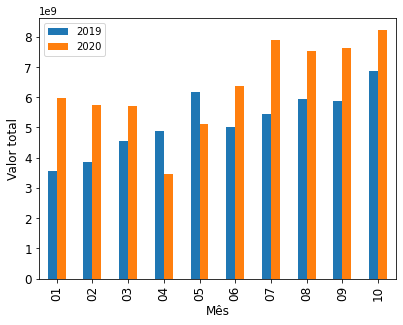
\includegraphics[scale=0.45]{images/base-de-dados-13.1-comparacao-valor-total-por-regiao.png}
        \caption{Região 1}
        \label{fig:pandemia:base-de-dados-13.1-comparacao-valor-total-por-regiao}
    \end{subfigure} ~ \quad
    \begin{subfigure}[b]{0.45\textwidth}
        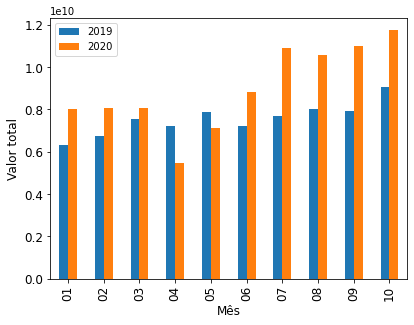
\includegraphics[scale=0.45]{images/base-de-dados-13.2-comparacao-valor-total-por-regiao.png}
        \caption{Região 2}
        \label{fig:pandemia:base-de-dados-13.2-comparacao-valor-total-por-regiao}
    \end{subfigure} ~ \\
    \begin{subfigure}[b]{0.45\textwidth}
        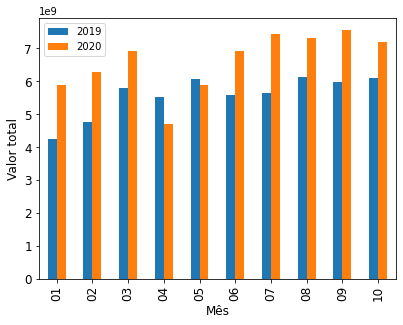
\includegraphics[scale=0.45]{images/base-de-dados-13.3-comparacao-valor-total-por-regiao.png}
        \caption{Região 3}
        \label{fig:pandemia:base-de-dados-13.3-comparacao-valor-total-por-regiao}
    \end{subfigure} ~ \quad
    \begin{subfigure}[b]{0.45\textwidth}
        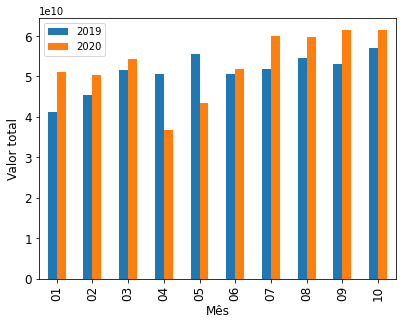
\includegraphics[scale=0.45]{images/base-de-dados-13.4-comparacao-valor-total-por-regiao.png}
        \caption{Região 4}
        \label{fig:pandemia:base-de-dados-13.4-comparacao-valor-total-por-regiao}
    \end{subfigure} ~ \\
    \begin{subfigure}[b]{0.45\textwidth} 
        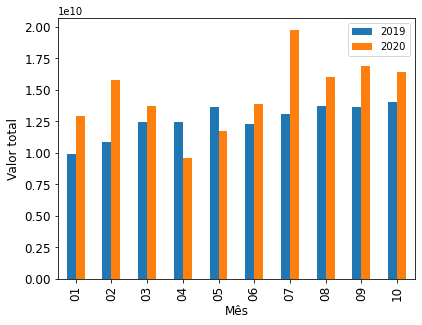
\includegraphics[scale=0.45]{images/base-de-dados-13.5-comparacao-valor-total-por-regiao.png}
        \caption{Região 5}
        \label{fig:pandemia:base-de-dados-13.5-comparacao-valor-total-por-regiao}
    \end{subfigure}
    \fdadospesquisa
\end{figure}

Na Figura~\ref{fig:pandemia:base-de-dados-14.1-valor-total-por-uf} vemos uma análise do valor total transacionado por UF no período de janeiro de 2019 e outubro de 2020. É possível observar um valor total transacionado consideravelmente maior no estado de São Paulo que, segundo descrição da seção~\ref{section:impacto:cenario-regional}, tem uma participação de 8\% do total das empresas deste estado, um percentual não muito diferente de outros estados citados. Outras UFs tem um valor total transacionado consideravelmente maior também, como Minas Gerais e Rio de Janeiro que reforçam a participação maior da região 4, e os estados da região 5 (sul): Paraná, Santa Catarina, e Rio Grande do Sul.

\begin{figure}[htb]
	\centering
    \caption{Valor total transacionado por UF no período analisado}
    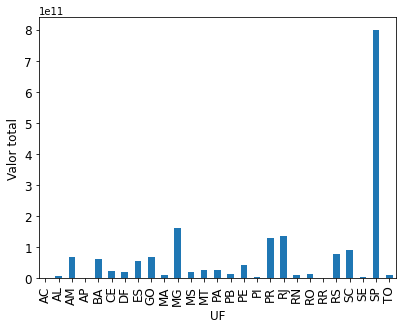
\includegraphics[scale=0.7]{images/base-de-dados-14.1-valor-total-por-uf.png}
    \label{fig:pandemia:base-de-dados-14.1-valor-total-por-uf}
    \fdadospesquisa
\end{figure}

A seguir, a Figura~\ref{fig:pandemia:base-de-dados-21.2-valor-trimestral-por-uf} apresenta graficamente uma comparação trimestral sobre o valor total transacionado em cada UF. Embora o valor total transacionado tenha grandes discrepâncias entre os estados, o que dificulta a identificação visual do impacto trimestral, é possível verificar que na maioria das UFs o valor total transacionado no segundo trimestre de 2020 é menor que no primeiro e no terceiro trimestre, o que indica um impacto maior devido à crise causada pela pandemia de COVID-19 nesse trimestre.

\begin{figure}[htb]
	\centering
    \caption{Valor trimestral transacionado por UF no período analisado}
    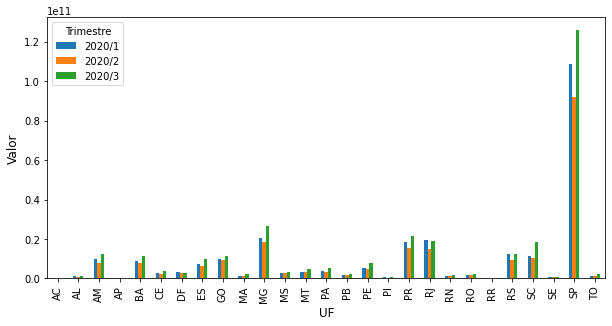
\includegraphics[scale=0.7]{images/base-de-dados-21.2-valor-trimestral-por-uf.png}
    \label{fig:pandemia:base-de-dados-21.2-valor-trimestral-por-uf}
    \fdadospesquisa
\end{figure}

Os dados são então detalhados na Tabela~\ref{tab:pandemia:variacao-mensal-por-uf}, onde é apresentada a diferença entre o valor mensal transacionado previsto para cada UF utilizando uma regressão linear sobre os dados entre janeiro de 2019 e fevereiro de 2020 e o valor real obtido para cada mês seguinte, de março a outubro de 2020.

\begin{table}[htb]
\centering
\caption{Diferença entre valores mensais transacionados previstos e obtidos por UF no período da pandemia}
\label{tab:pandemia:variacao-mensal-por-uf}
    \begin{tabular}{c|r|r|r|r|r|r|r|r}
        \toprule
        \textbf{UF} & Março & Abril & Maio & Junho & Julho & Agosto & Setembro & Outubro \\
        \midrule
        \textbf{AC} &  -7.3\% & -33.9\% &  -5.1\% &   9.2\% &   27.3\% &    20.5\% &    20.6\% &   15.4\% \\
        \textbf{AL} & -11.0\% & -33.6\% & -26.5\% & -12.3\% &    6.9\% &     3.9\% &    15.4\% &    9.0\% \\
        \textbf{AM} & -15.8\% & -62.5\% & -31.5\% & -14.3\% &    0.5\% &    -4.5\% &    -8.4\% &    4.1\% \\
        \textbf{AP} & -15.6\% & -29.1\% & -17.5\% &  -8.1\% &   17.4\% &    23.9\% &    22.1\% &   12.9\% \\
        \textbf{BA} &  -0.4\% & -36.0\% & -21.7\% &  -3.3\% &   11.0\% &     4.9\% &    12.7\% &   13.5\% \\
        \textbf{CE} & -15.6\% & -45.1\% & -26.3\% &  -7.7\% &   10.8\% &     7.6\% &     7.4\% &   19.1\% \\
        \textbf{DF} &  32.3\% & -18.6\% & -19.0\% &  16.4\% &    9.8\% &     2.8\% &    10.7\% &    6.6\% \\
        \textbf{ES} &  -6.5\% & -40.1\% & -24.2\% &  -5.8\% &    6.1\% &     5.6\% &    16.2\% &    6.4\% \\
        \textbf{GO} &  10.8\% & -29.5\% &  -7.9\% &   4.0\% &    9.5\% &     1.3\% &     7.3\% &    0.4\% \\
        \textbf{MA} & -20.9\% & -31.2\% & -24.8\% &   0.2\% &   22.3\% &    21.2\% &     6.8\% &   13.7\% \\
        \textbf{MG} &  -9.0\% & -35.1\% & -20.6\% &  -6.7\% &   12.2\% &     9.1\% &    12.0\% &   11.1\% \\
        \textbf{MS} &   3.4\% & -16.0\% &  -9.1\% &  -1.6\% &   12.8\% &     5.8\% &    -3.5\% &  -15.3\% \\
        \textbf{MT} & -13.3\% & -38.9\% & -13.4\% &  -3.2\% &    7.0\% &    24.5\% &    19.8\% &   17.0\% \\
        \textbf{PA} & -13.6\% & -33.3\% & -25.8\% &  -8.8\% &   18.5\% &     5.9\% &     9.7\% &    6.1\% \\
        \textbf{PB} &  -8.7\% & -38.5\% & -11.6\% &   1.7\% &   36.1\% &    15.8\% &    20.2\% &   30.7\% \\
        \textbf{PE} & -14.6\% & -43.4\% & -21.0\% &  -7.9\% &   17.5\% &    15.8\% &    11.8\% &   23.9\% \\
        \textbf{PI} & -10.6\% & -47.1\% & -24.5\% &  -7.0\% &   25.2\% &    13.4\% &    24.3\% &   15.1\% \\
        \textbf{PR} &  -2.2\% & -37.2\% & -22.8\% & -11.5\% &    1.5\% &    -0.7\% &     1.4\% &   -2.0\% \\
        \textbf{RJ} &  -6.7\% & -43.6\% & -25.6\% & -17.2\% &   -8.6\% &   -10.4\% &   -17.7\% &  -17.7\% \\
        \textbf{RN} & -14.9\% & -47.3\% & -39.7\% & -23.3\% &   10.6\% &     8.1\% &    24.7\% &   31.9\% \\
        \textbf{RO} &  -3.0\% & -25.2\% & -10.0\% &  -4.7\% &   17.1\% &     2.1\% &    -0.1\% &   -4.8\% \\
        \textbf{RR} &  82.5\% &  90.6\% & 189.3\% & 370.4\% & 1480.1\% & - & - & - \\
        \textbf{RS} & -18.4\% & -42.0\% & -33.7\% & -20.1\% &   -7.9\% &   -17.9\% &   -15.0\% &  -23.9\% \\
        \textbf{SC} &  -8.2\% & -32.5\% & -18.8\% &  -6.3\% &   89.5\% &    12.3\% &    20.3\% &   19.7\% \\
        \textbf{SE} &  -4.2\% & -38.7\% &   6.2\% &  23.9\% &   16.0\% &    13.6\% &     7.4\% &   26.6\% \\
        \textbf{SP} &  -0.9\% & -32.9\% & -24.1\% &  -9.9\% &    3.0\% &     1.9\% &     4.6\% &    4.1\% \\
        \textbf{TO} & -13.4\% & -32.1\% & -18.9\% &   2.4\% &   18.4\% &    13.9\% &    23.7\% &   19.7\% \\
        \bottomrule
    \end{tabular}
\nota{Os dados de Roraima foram insuficientes para uma previsão correta e registraram valores com bastante ruído, fazendo com que a previsão de valores utilizando a regressão linear indicasse valores bastante pessimistas para os meses da pandemia. Foram mantidos os valores de março a julho e removidos os valores posteriores devido ao ruído. Da mesma forma, consideramos que o estado de Roraima não foi impactado negativamente pela pandemia}
\fdadospesquisa
\end{table}

É possível observar que apenas o estado de Roraima não foi afetado pela crise segundo essa análise, mas como indicado na Tabela~\ref{tab:pandemia:variacao-mensal-por-uf} os dados desse estado não possuem um ruído considerável. Todos as outras UFs apresentaram pelo menos um mês cujo valor transacionado previsto e real indicam impacto negativo da crise. Os meses que concentram maior impacto novamente são os meses de março a junho, novamente indicando que o segundo de trimestre de 2020 foi o mais impactado pela pandemia.

Na Tabela~\ref{tab:pandemia:variacao-total-por-uf} apresentamos a diferença entre o valor total previsto e obtido para o período de março a outubro de 2020.

\begin{table}[htb]
\centering
\caption{Diferença entre valores totais transacionados previstos e obtidos por UF no período da pandemia}
\label{tab:pandemia:variacao-total-por-uf}
    \begin{tabular}{l|r}
        \toprule
        \textbf{UF} & Variação total \\
        \midrule
        \textbf{AC} &   6.2\% \\
        \textbf{AL} &  -5.5\% \\
        \textbf{AM} & -15.7\% \\
        \textbf{AP} &   1.3\% \\
        \textbf{BA} &  -1.8\% \\
        \textbf{CE} &  -5.7\% \\
        \textbf{DF} &   5.1\% \\
        \textbf{ES} &  -4.9\% \\
        \textbf{GO} &  -0.4\% \\
        \textbf{MA} &  -0.7\% \\
        \textbf{MG} &  -3.1\% \\
        \textbf{MS} &  -2.9\% \\
        \textbf{MT} &   0.4\% \\
        \textbf{PA} &  -4.6\% \\
        \textbf{PB} &   5.9\% \\
        \textbf{PE} &  -1.7\% \\
        \textbf{PI} &  -0.7\% \\
        \textbf{PR} &  -8.9\% \\
        \textbf{RJ} & -18.4\% \\
        \textbf{RN} &  -6.1\% \\
        \textbf{RO} &  -3.4\% \\
        \textbf{RR} & 484.7\% \\
        \textbf{RS} & -22.1\% \\
        \textbf{SC} &  10.0\% \\
        \textbf{SE} &   6.6\% \\
        \textbf{SP} &  -6.6\% \\
        \textbf{TO} &   2.5\% \\
        \bottomrule
    \end{tabular}
\fdadospesquisa
\end{table}

É possível verificar que dezoito UFs tiveram impacto no valor total transacionado em relação ao previsto, sendo os mais afetados o Rio Grande do Sul, o Rio de Janeiro, e o Amazonas. Nove UFs tiveram um valor previsto menor que o obtido, o que segundo esta análise significa que a retomada para estes estados pode ter compensado as perdas dos meses mais críticos.

Na Tabela~\ref{tab:pandemia:impacto-por-uf} é descrita a quantidade de UFs impactada mensalmente e totalmente no período analisado. Consideramos aqui que o impacto mensal significa que pelo menos um mês teve um valor transacionado obtido 25\% menor que o valor previsto, e impacto total indica que o valor total obtido foi menor que o previsto.

\begin{table}[htb]
\centering
\caption{Quantidade de UFs impactadas negativamente pela pandemia em relação às variações mensais ou totais}
\label{tab:pandemia:impacto-por-uf}
    \begin{tabular}{l|r|r}
        \toprule
        Impacto & Mensal & Total \\
        \midrule
        Sim & 24 & 18 \\
        Não &  3 &  9 \\
        \bottomrule
    \end{tabular}
\fdadospesquisa
\end{table}

\section{Cenário econômico}
\label{section:impacto:cenario-economico}

Nesta seção, serão apresentados os resultados da análise de impacto da pandemia de COVID-19 na economia do ponto de vista setorial. Para isso, vamos usar o CNAE para segmentar a economia, como descrito na seção~\ref{section:base-de-dados:analise-descritiva:abrangencia-economica}.

Na Figura~\ref{fig:pandemia:base-de-dados-15.1-valor-total-por-secao} é apresentado o volume transacionado por seção de CNAE considerando o total entre janeiro de 2019 e outubro de 2020.

\begin{figure}[htb]
	\centering
    \caption{Valor total transacionado por seção no período analisado}
    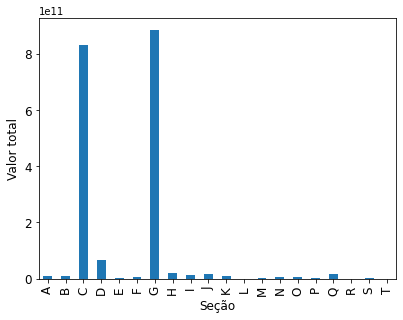
\includegraphics[scale=0.7]{images/base-de-dados-15.1-valor-total-por-secao.png}
    \label{fig:pandemia:base-de-dados-15.1-valor-total-por-secao}
    \fdadospesquisa
\end{figure}

A partir desses dados, podemos ver um volume muito maior transacionado nas seções C e G do CNAE, respectivamente as seções de "Indústria de Transformação" e "Comércio; Reparação de veículos automotores e motocicletas". Como pudemos ver na seção~\ref{section:base-de-dados:analise-descritiva:abrangencia-economica}, as seções C e G apresentam uma participação um pouco maior que as demais na base de dados, sendo que a seção G possui uma quantidade bastante grande de empresas também na base de referência em relação às demais, fato correspondido também aqui.

Na Figura~\ref{fig:pandemia:base-de-dados-22-valor-trimestral-por-secao} repetimos a análise trimestral agora por seção, ilustrando os valores transacionados nos três primeiros trimestres de 2020 para cada seção. Como as seções C e G possuem volumes muito maiores, é difícil visualizar o impacto para todas as seções, mas podemos verificar a mesma tendência encontrada até aqui: o segundo trimestre de 2020 apresentou um impacto negativo em relação ao primeiro e ao terceiro trimestres, com acentuada queda o volume transacionado total.

\begin{figure}[htb]
	\centering
    \caption{Valor trimestral transacionado por seção no período analisado}
    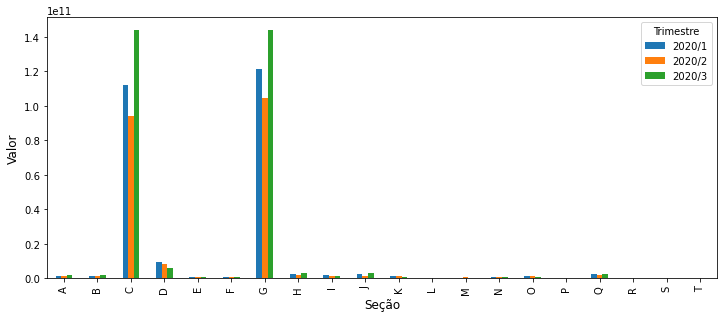
\includegraphics[scale=0.7]{images/base-de-dados-22-valor-trimestral-por-secao.png}
    \label{fig:pandemia:base-de-dados-22-valor-trimestral-por-secao}
    \fdadospesquisa
\end{figure}

Na Tabela~\ref{tab:pandemia:variacao-mensal-por-secao} é descrito em detalhes a diferença entre o valor previsto via regressão linear aplicada aos dados de valor mensal transacionado entre janeiro de 2019 a fevereiro de 2020 para os meses de março a outubro de 2020 e o valor obtido nesses meses.

\begin{table}[htb]
\centering
\caption{Diferença entre valores mensais transacionados previstos e obtidos por seção no período da pandemia}
\label{tab:pandemia:variacao-mensal-por-secao}
    \begin{tabular}{c|r|r|r|r|r|r|r|r}
        \toprule
        \textbf{Seção} & Março & Abril & Maio & Junho & Julho & Agosto & Setembro & Outubro \\
        \midrule
        \textbf{A} & -15.4\% & -24.4\% & -14.2\% & -10.8\% &   6.9\% &   8.2\% &  32.9\% &  28.6\% \\
        \textbf{B} &   2.8\% &  12.8\% &  19.1\% &  32.7\% &  50.6\% &  51.0\% &  58.5\% &  64.6\% \\
        \textbf{C} &  -4.2\% & -39.0\% & -23.6\% &  -5.8\% &  16.0\% &  11.7\% &  15.5\% &  16.2\% \\
        \textbf{D} &  -1.4\% &  -6.1\% & -16.7\% & -14.4\% & -12.8\% & -39.3\% & -62.2\% & -64.5\% \\
        \textbf{E} &  10.8\% & -32.0\% & -17.3\% &  17.1\% &  65.5\% & 125.2\% &  -1.3\% &  15.3\% \\
        \textbf{F} &  -4.7\% & -30.0\% & -26.8\% & -20.0\% &  -8.1\% & -13.8\% & -10.0\% & -15.0\% \\
        \textbf{G} &  -5.9\% & -36.8\% & -23.0\% & -11.6\% &   4.0\% &  -2.3\% &  -0.2\% &  -2.3\% \\
        \textbf{H} & -16.2\% & -40.0\% & -39.2\% & -24.5\% & -17.0\% & -15.5\% &  -7.0\% &  -9.7\% \\
        \textbf{I} & -25.8\% & -53.7\% & -51.7\% & -42.2\% & -33.1\% & -33.4\% & -27.9\% & -25.3\% \\
        \textbf{J} &  24.3\% & -61.6\% & -47.4\% & -32.3\% &  -6.4\% &  -5.3\% & -19.3\% &   5.4\% \\
        \textbf{K} &   4.6\% &  15.1\% &  12.6\% &  13.2\% &  14.2\% & -72.6\% & -64.8\% & -66.1\% \\
        \textbf{L} & -28.3\% & -34.7\% & -56.8\% & -51.3\% & -49.2\% & -29.1\% & -34.2\% & -57.0\% \\
        \textbf{M} & -12.2\% & -12.2\% &  57.9\% &  71.4\% & -33.2\% & -32.2\% & -16.3\% & -12.8\% \\
        \textbf{N} &  -1.6\% & -52.1\% & -42.2\% & -10.0\% &  28.9\% &  -4.7\% &   5.7\% &   1.9\% \\
        \textbf{O} &  53.8\% &  20.7\% &   2.8\% &  77.7\% &  11.1\% &  -4.6\% &  27.2\% & -28.1\% \\
        \textbf{P} & -12.0\% & -56.8\% & -44.6\% & -33.5\% & -22.1\% & -34.0\% & -31.3\% & -39.5\% \\
        \textbf{Q} &  33.1\% & -10.5\% &  -6.4\% &  -7.2\% &   6.7\% &  -3.9\% &   2.7\% & -11.2\% \\
        \textbf{R} & -32.2\% & -68.9\% & -69.6\% & -50.6\% & -42.7\% & -41.5\% & -18.5\% & -18.3\% \\
        \textbf{S} &  -5.4\% & -32.9\% & -24.7\% & -22.5\% & -10.4\% & -19.5\% &   2.0\% &  -0.2\% \\
        \textbf{T} & -40.5\% & -38.2\% & -61.9\% & -48.5\% & -47.5\% & -54.7\% & -54.2\% & -27.6\% \\
        \bottomrule
    \end{tabular}
\fdadospesquisa
\end{table}

Podemos verificar que a maior parte do impacto na maioria das seções da economia se dá entre março e junho de 2020, com perdas significativas registradas neste período para várias seções. Ao contrário de outras análises até aqui, podemos verificar que algumas seções da economia foram pouco impactadas e apresentaram resultados positivos no período estudado. A seção B, de indústrias extrativas, apresentou resultados positivos em todo o período estudado. Outras seções apresentaram um impacto negativo estendido para todos os meses, sendo estas as seções D, F, H, L, P, R, e T.

A Tabela~\ref{tab:pandemia:variacao-total-por-secao} apresenta a diferença entre o valor total previsto e obtido para o período estudado. As seçõs B e O, respectivamente referentes a Indústrias Extrativas e Administração pública, foram aquelas em que o impacto foi positivo, obtendo um valor maior que o previsto, enquanto outras seções foram severamente impactadas, como L, R, T, respectivamente referentes a Atividades Imobiliárias, Artes, Cultura e Esporte, e Serviços Domésticos.

\begin{table}[htb]
\centering
\caption{Diferença entre valores totais transacionados previstos e obtidos por seção no período da pandemia}
\label{tab:pandemia:variacao-total-por-secao}
    \begin{tabular}{l|r}
        \toprule
        \textbf{Seção} & Variação total \\
        \midrule
        \textbf{A} &   2.4\% \\
        \textbf{B} &  36.0\% \\
        \textbf{C} &  -1.3\% \\
        \textbf{D} & -27.0\% \\
        \textbf{E} &  23.5\% \\
        \textbf{F} & -16.0\% \\
        \textbf{G} &  -9.5\% \\
        \textbf{H} & -20.8\% \\
        \textbf{I} & -36.5\% \\
        \textbf{J} & -17.4\% \\
        \textbf{K} & -17.7\% \\
        \textbf{L} & -42.8\% \\
        \textbf{M} &   0.5\% \\
        \textbf{N} &  -9.1\% \\
        \textbf{O} &  20.8\% \\
        \textbf{P} & -34.2\% \\
        \textbf{Q} &   0.3\% \\
        \textbf{R} & -42.7\% \\
        \textbf{S} & -14.0\% \\
        \textbf{T} & -46.6\% \\
        \bottomrule
    \end{tabular}
\fdadospesquisa
\end{table}

A Tabela~\ref{tab:pandemia:impacto-por-secao} apresenta a consolidação da categorização de seções quanto ao impacto mensal e total. Novamente, impacto mensal se refere às seções cujo o valor obtido foi 25\% menor que o previsto para pelo menos um mês da pandemia, e impacto total se o valor total obtido para o período foi menor que o previsto.

\begin{table}[htb]
\centering
\caption{Quantidade de seções impactadas negativamente pela pandemia em relação às variações mensais ou totais}
\label{tab:pandemia:impacto-por-secao}
    \begin{tabular}{l|r|r}
        \toprule
        Impacto & Mensal & Total \\
        \midrule
        Sim & 17 & 14 \\
        Não &  3 &  6 \\
        \bottomrule
    \end{tabular}
\fdadospesquisa
\end{table}

A Figura~\ref{fig:pandemia:base-de-dados-23.1-valor-total-por-cnae} estende a análise para um estudo do impacto por CNAE. Ela apresenta um diargama de caixas dos valores mensais transacionados por CNAE entre janeiro de 2019 e outubro de 2020.

\begin{figure}[htb]
	\centering
    \caption{Histograma do valor total transacionado por CNAE no período analisado}
    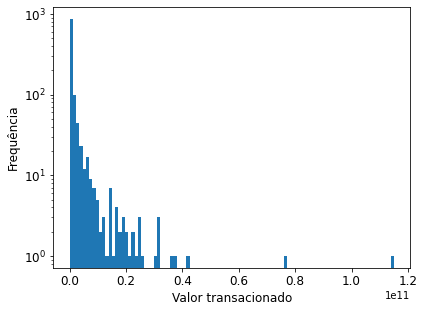
\includegraphics[scale=0.7]{images/base-de-dados-23.1-valor-total-por-cnae.png}
    \label{fig:pandemia:base-de-dados-23.1-valor-total-por-cnae}
    \fdadospesquisa
\end{figure}

Os dados de valores transacionados por CNAE tem grande variância, o que dificulta uma análise, mas é possível ver através do histograma que novamente os meses de abril e maio possuem uma distribuição de valores ligeiramente menor que o restante, mantendo o padrão anterior.

\begin{figure}[htb]
	\centering
    \caption{Diagrama de caixa dos valores mensais transacionados por CNAE no período analisado}
    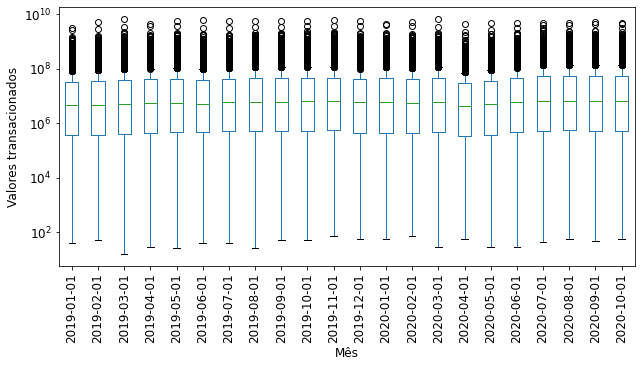
\includegraphics[scale=0.7]{images/base-de-dados-23.2-valor-mensal-por-cnae.png}
    \label{fig:pandemia:base-de-dados-23.2-valor-mensal-por-cnae}
    \fdadospesquisa
\end{figure}

Sobre os dados de CNAE também foi aplicada uma regressão linear sobre os dados obtidos nos meses de janeiro de 2019 a fevereiro de 2020 para a previsão dos valores para os meses de março de a outubro de 2020. Da mesma forma, a Tabela~\ref{tab:pandemia:impacto-por-cnae} mostra uma categorização de impacto mensal e total para CNAEs usando os mesmos critérios apresentados anteriormente: é considerado impacto mensal aquele onde para um determinado mês o valor obtido é 25\% menor que o valor previsto, e impacto total se o valor total obtido é menor que o previsto.

\begin{table}[htb]
\centering
\caption{Quantidade de CNAEs impactadas negativamente pela pandemia em relação às variações mensais ou totais}
\label{tab:pandemia:impacto-por-cnae}
    \begin{tabular}{l|r|r}
        \toprule
        Impacto & Mensal & Total \\
        \midrule
        Sim & 852 & 600 \\
        Não & 273 & 525 \\
        \bottomrule
    \end{tabular}
\fdadospesquisa
\end{table}

\section{Conclusões}
\label{section:impacto:conclusoes}

Finalizamos então a análise de impacto para diferentes segmentações, e pudemos verificar que em todos os cenários houve algum impacto entre os valores previstos e obtidos. Foi apresentada uma análise comparativa entre 2019 e 2020, e uma análise usando uma previsão de valor transacionado e valor real obtido. O impacto foi mais localizado entre os meses de março e junho, tornando o segundo trimestre de 2020 o mais afetado.

Cada cenário possui proporções diferentes de entidades afetadas e não afetadas pela pandemia, com um desbalanceamento maior para entidades afetadas. O objetivo, portanto, foi apresentar uma categorização das entidades ao mesmo tempo que aprofundamos a análise do Capítulo~\ref{chapter:base-de-dados} para mostrar sob o ponto de vista de valores transacionados uma nova perspectiva dos dados aqui apresentados.


\chapter{Resultados}
\label{chapter:resultados}

Neste capítulo, serão apresentados os resultados obtidos a partir da aplicação do que foi proposto na seção~\ref{introducao:objetivos}, seguido de uma análise dos dados.

\section{Caracterização de redes}
\label{section:metricas-redes}

Neste capítulo, faremos uma caracterização dos dados a partir de diferentes modelagens utilizando redes complexas.

\subsection{Redes UF-UF}
\label{section:metricas-redes:uf}

Nesta seção, será apresentada a caracterização de uma rede entre unidades federativas brasileiras.

\begin{table}[htb]
\centering
\caption{Métricas do grafo de transações entre UFs}
\label{tab:metricas-redes:grafo-por-uf}
    \begin{tabular}{l|r}
    \toprule
    Métrica &  Valor \\
    \midrule
    Quantidade de nós         &  27      \\
    Quantidade de arestas     & 377      \\
    Diâmetro                  &   2      \\
    Raio                      &   1      \\
    Grau médio                &  26.9259 \\
    Densidade                 &   1.0740 \\
    Transitividade            &   0.9971 \\
    Assortatividade de grau   &  -0.0356 \\
    Assortatividade de região &  -0.0025 \\
    \bottomrule
    \end{tabular}
\fdadospesquisa
\end{table}

Essa rede foi montada utilizando os dados de transações entre janeiro de 2019 e dezembro de 2019. Cada vértice representa uma UF e cada aresta representa o valor total transacionado no período entre duas UFs. Nesta modelagem consideramos um grafo não-direcionado cíclico. Cada vértice possui um atributo chamado \textbf{região} indicando a região a que pertence aquela UF. Cada aresta além do atributo contendo o valor total transacional, e um atributo chamado \textbf{distância} correspondente ao inverso do valor total transacionado. Este atributo reflete a distância econômica entre dois vértices, uma vez que vértices que tenham um alto valor transacionado entre si terão uma relação mais próxima, o que pode ser útil na formulação de alguns algoritmos. A Tabela~\ref{tab:metricas-redes:grafo-por-uf} apresenta as métricas do grafo para esta modelagem.

\begin{table}[htb]
\centering
\caption{Métricas do grafo de transações entre UFs segmentadas por UF}
\label{tab:metricas-redes:grafo-por-uf-especificas1}
    \begin{tabular}{l|rrrrrr}
    \toprule
    UF & Grau & \shortstack{Coeficiente\\de agrupamento} &  \shortstack{Caminho mínimo\\ médio poderado} & \shortstack{Centralidade\\de informação} &  \shortstack{Centralidade\\de autovalor} &  \textit{PageRank} \\
    \midrule
    AC & 26 & 0.0003 & $2.61e^{-09}$ & $4.51e^{+07}$ & 0.0016 & 0.0077 \\
    AL & 27 & 0.0008 & $1.07e^{-09}$ & $1.15e^{+08}$ & 0.0057 & 0.0112 \\
    AM & 27 & 0.0045 & $5.06e^{-10}$ & $2.33e^{+08}$ & 0.0714 & 0.0468 \\
    AP & 26 & 0.0005 & $2.66e^{-09}$ & $5.57e^{+07}$ & 0.0016 & 0.0077 \\
    BA & 27 & 0.0030 & $5.27e^{-10}$ & $2.16e^{+08}$ & 0.0538 & 0.0348 \\
    CE & 27 & 0.0019 & $6.39e^{-10}$ & $1.81e^{+08}$ & 0.0199 & 0.0185 \\
    DF & 27 & 0.0015 & $5.74e^{-10}$ & $1.83e^{+08}$ & 0.0290 & 0.0162 \\
    ES & 27 & 0.0033 & $5.03e^{-10}$ & $2.24e^{+08}$ & 0.0801 & 0.0334 \\
    GO & 27 & 0.0037 & $5.17e^{-10}$ & $2.25e^{+08}$ & 0.0634 & 0.0401 \\
    MA & 27 & 0.0012 & $8.34e^{-10}$ & $1.46e^{+08}$ & 0.0093 & 0.0131 \\
    MG & 27 & 0.0054 & $4.82e^{-10}$ & $2.39e^{+08}$ & 0.1696 & 0.0744 \\
    MS & 27 & 0.0015 & $5.96e^{-10}$ & $1.75e^{+08}$ & 0.0249 & 0.0153 \\
    MT & 27 & 0.0019 & $6.21e^{-10}$ & $1.85e^{+08}$ & 0.0219 & 0.0204 \\
    PA & 27 & 0.0021 & $5.89e^{-10}$ & $1.90e^{+08}$ & 0.0261 & 0.0216 \\
    PB & 27 & 0.0014 & $7.46e^{-10}$ & $1.58e^{+08}$ & 0.0124 & 0.0140 \\
    PE & 27 & 0.0029 & $5.59e^{-10}$ & $2.14e^{+08}$ & 0.0339 & 0.0325 \\
    PI & 27 & 0.0007 & $1.37e^{-09}$ & $9.40e^{+07}$ & 0.0039 & 0.0084 \\
    PR & 27 & 0.0049 & $4.85e^{-10}$ & $2.37e^{+08}$ & 0.1416 & 0.0630 \\
    RJ & 27 & 0.0051 & $4.82e^{-10}$ & $2.38e^{+08}$ & 0.1596 & 0.0659 \\
    RN & 27 & 0.0011 & $8.10e^{-10}$ & $1.33e^{+08}$ & 0.0097 & 0.0125 \\
    RO & 27 & 0.0010 & $8.09e^{-10}$ & $1.45e^{+08}$ & 0.0100 & 0.0138 \\
    RR & 27 & 0.0003 & $1.83e^{-09}$ & $4.51e^{+07}$ & 0.0009 & 0.0067 \\
    RS & 27 & 0.0038 & $5.16e^{-10}$ & $2.26e^{+08}$ & 0.0680 & 0.0416 \\
    SC & 27 & 0.0042 & $4.97e^{-10}$ & $2.31e^{+08}$ & 0.0971 & 0.0474 \\
    SE & 27 & 0.0006 & $1.64e^{-09}$ & $9.23e^{+07}$ & 0.0025 & 0.0091 \\
    SP & 27 & 0.0119 & $4.59e^{-10}$ & $2.52e^{+08}$ & 0.9426 & 0.3101 \\
    TO & 27 & 0.0011 & $8.96e^{-10}$ & $1.42e^{+08}$ & 0.0085 & 0.0127 \\
    \bottomrule
    \end{tabular}
\fdadospesquisa
\end{table}

É possível notar que o grafo entre UFs é quase completo, com alto grau médio, refletindo o baixo diâmetro e raio da rede. Dado que estamos usando uma modelagem cíclica, aceitando arestas que conectam um vértice a ele mesmo, a densidade desta rede é maior que $1.0$. Temos também alta transitividade, e baixa assortatividade de grau e de região. Por ser um grafo bastante completo, é difícil tomar qualquer conclusão a partir destas métricas uma vez que elas irão refletir a simplicidade da topologia desta rede.

A Tabela~\ref{tab:metricas-redes:grafo-por-cnae-especificas1} nos dá uma ideia melhor da topologia do grafo. Para essas métricas agora consideramos a formulação usando arestas ponderadas pelo valor total transacionado pelas UFs. Para os caminhos mínimos, foi utilizada a distância entre UFs, como definido anteriormente.

Todos as UFs estão conectadas entre si com uma exceção: o estado do Acre não possui conexão com o estado do Amapá. O estado de Sâo Paulo se sobressai com maiores valores de coeficiente de agrupamento, centralidade de autovalor, e pagerank por ter um maior valor transacionado entre este estado e todos os outros se comparado aos demais, algo que já foi descrito na seção~\ref{chapter:impacto-economico}. Observando outros estados da região sudeste, como Rio de Janeiro de Minas Gerais, estes também tem valores importantes para essas métricas mostrando sua importância, novamente refletindo a tendência dessa região de se sobressair quanto ao valor transacionado e influenciando positivamente nestas métricas. Os estados da região norte, como Acre, Amapá, e Roraima apresentaram baixos valores para estas métricas refletindo os baixos valores transacionados por estas UFs com as demais. Sendo assim, apesar de uma topologia simples, ela se mostra razoavelmente eficaz em mostrar a importância de cada estado em relação às relações econômicas entre UFs brasileiras, também obedecendo às limitações e ao viés desta base de dados.

Nesta análise, não consideramos as métricas de centralidade de intermediação, caminho mínimo médio, e excentricidade, uma vez que o grafo é quase completo e essas medidas refletiriam apenas o grau de cada vértice, apresentando pouca variância e sendo redundante com o restando dos dados obtidos.

\subsection{Redes Seção-Seção}
\label{section:metricas-redes:secao}

Nesta seção, será apresentada a caracterização de uma rede entre seções de CNAE.

\begin{table}[htb]
\centering
\caption{Métricas do grafo de transações entre seções}
\label{tab:metricas-redes:grafo-por-secao}
    \begin{tabular}{l|r}
    \toprule
    Métrica &  Valor \\
    \midrule
    Quantidade de nós       &   20      \\
    Quantidade de arestas   &  186      \\
    Diâmetro                &    2      \\
    Raio                    &    1      \\
    Grau médio              &   17.6000 \\
    Densidade               &    0.9789 \\
    Transitividade          &    0.9618 \\
    Assortatividade de grau &   -0.1433 \\
    \bottomrule
    \end{tabular}
\fdadospesquisa
\end{table}

Essa rede foi montada utilizando os dados de transações entre janeiro de 2019 e dezembro de 2019, como anteriormente. Cada vértice representa uma seção e cada aresta representa o valor total transacionado no período entre duas seções. Nesta modelagem consideramos novamente um grafo não-direcionado cíclico. Cada aresta possui também um atributo chamado \textbf{distância} correspondente ao inverso do valor total transacionado. A Tabela~\ref{tab:metricas-redes:grafo-por-secao} apresenta as métricas do grafo para esta modelagem.

Podemos observar que este grafo não é tão completo quanto o o grafo UF-UF, mas também é bastante completo com um alto grau médio e densidade, encurtando os valores de raio e diâmetro. A assortatividade de grau indica leve tendência à assortatividade negativa, indicando alguma tendência de vértices menos conectados se conectarem à vértices mais conectados e vice-versa, uma característica que reflete também a própria topologia dessa rede, com pouca variância entre o grau de seus vértice uma vez que é uma rede bastante conectada.

As Tabelas~\ref{tab:metricas-redes:grafo-por-secao-especificas1} e \ref{tab:metricas-redes:grafo-por-secao-especificas2} detalham as métricas agora por seção, sendo novamente considerada a formulação usando arestas ponderadas e utilizando a distância entre seções para a formulação de caminhos mínimos ponderados.

\begin{table}[htb]
\centering
\caption{Métricas do grafo de transações entre seções segmentadas por seção (Parte 1)}
\label{tab:metricas-redes:grafo-por-secao-especificas1}
    \begin{tabular}{l|rrrr}
    \toprule
    Seção &  Grau &  \shortstack{Coeficiente\\de agrupamento} &  \shortstack{Caminho\\mínimo médio} &  \shortstack{Caminho mínimo\\médio ponderado} \\
    \midrule
    A &  19 &          0.0006 &     1 &  $1.635e^{-06}$ \\
    B &  19 &          0.0007 &     1 &  $1.635e^{-06}$ \\
    C &  20 &          0.0047 &  0.95 &  $1.634e^{-06}$ \\
    D &  19 &          0.0010 &     1 &  $1.634e^{-06}$ \\
    E &  19 &          0.0003 &     1 &  $1.635e^{-06}$ \\
    F &  19 &          0.0005 &     1 &  $1.635e^{-06}$ \\
    G &  20 &          0.0048 &  0.95 &  $1.634e^{-06}$ \\
    H &  19 &          0.0010 &     1 &  $1.634e^{-06}$ \\
    I &  19 &          0.0008 &     1 &  $1.634e^{-06}$ \\
    J &  19 &          0.0009 &     1 &  $1.634e^{-06}$ \\
    K &  17 &          0.0005 &   1.1 &  $1.635e^{-06}$ \\
    L &  15 &         >0.0001 &   1.2 &  $1.648e^{-06}$ \\
    M &  19 &          0.0002 &     1 &  $1.635e^{-06}$ \\
    N &  19 &          0.0005 &     1 &  $1.635e^{-06}$ \\
    O &  18 &          0.0005 &  1.05 &  $1.634e^{-06}$ \\
    P &  18 &          0.0001 &  1.05 &  $1.637e^{-06}$ \\
    Q &  19 &          0.0008 &     1 &  $1.634e^{-06}$ \\
    R &  15 &         >0.0001 &   1.1 &  $1.646e^{-06}$ \\
    S &  19 &          0.0002 &     1 &  $1.635e^{-06}$ \\
    T &   1 &         >0.0001 &   1.8 &  $3.102e^{-05}$ \\
    \bottomrule
    \end{tabular}
\fdadospesquisa
\end{table}

\begin{table}[htb]
\centering
\caption{Métricas do grafo de transações entre seções segmentadas por seção (Parte 2)}
\label{tab:metricas-redes:grafo-por-secao-especificas2}
    \begin{tabular}{l|rrrrr}
    \toprule
    Seção & \shortstack{Centralidade\\de informação} &  \shortstack{Centralidade\\de autovalor} &   \shortstack{Centralidade\\de intermediação} & \shortstack{Centralidade\\de proximidade} & PageRank \\
    \midrule
    A & $3.907e^{+04}$ &  0.0116 &  0.0020 &  0.95 &  0.0131 \\
    B & $3.907e^{+04}$ &  0.0090 &  0.0020 &  0.95 &  0.0132 \\
    C & $3.907e^{+04}$ &  0.6961 &  0.0517 &  1    &  0.3633 \\
    D & $3.907e^{+04}$ &  0.0139 &  0.0020 &  0.95 &  0.0457 \\
    E & $3.906e^{+04}$ &  0.0038 &  0.0020 &  0.95 &  0.0093 \\
    F & $3.906e^{+04}$ &  0.0067 &  0.0020 &  0.95 &  0.0110 \\
    G & $3.907e^{+04}$ &  0.7167 &  0.0517 &  1    &  0.3954 \\
    H & $3.907e^{+04}$ &  0.0213 &  0.0020 &  0.95 &  0.0171 \\
    I & $3.907e^{+04}$ &  0.0123 &  0.0020 &  0.95 &  0.0143 \\
    J & $3.907e^{+04}$ &  0.0173 &  0.0020 &  0.95 &  0.0169 \\
    K & $3.907e^{+04}$ &  0.0032 &  0      &  0.86 &  0.0147 \\
    L & $3.887e^{+04}$ &  0.0001 &  0      &  0.79 &  0.0075 \\
    M & $3.905e^{+04}$ &  0.0020 &  0.0020 &  0.95 &  0.0090 \\
    N & $3.906e^{+04}$ &  0.0066 &  0.0020 &  0.95 &  0.0105 \\
    O & $3.907e^{+04}$ &  0.0085 &  0.0003 &  0.90 &  0.0113 \\
    P & $3.903e^{+04}$ &  0.0006 &  0.0003 &  0.90 &  0.0078 \\
    Q & $3.907e^{+04}$ &  0.0177 &  0.0020 &  0.95 &  0.0156 \\
    R & $3.881e^{+04}$ &  0.0001 &  0      &  0.86 &  0.0075 \\
    S & $3.905e^{+04}$ &  0.0016 &  0.0020 &  0.95 &  0.0084 \\
    T & $2.058e^{+03}$ &  4.826e &  0      &  0.53 &  0.0075 \\
    \bottomrule
    \end{tabular}
\fdadospesquisa
\end{table}

Podemos observar que assim como anteriormente, as seções C e G se sobressaem com altos valores de agrupamento e centralidade, indicando influencia dos altos valores transacionados por essas seções com outras regiões. A seção T se sobressai com uma baixa conectividade com outras seções, e as seções L e R são bastante influenciadas pelos baixos valores transacionados. O caminho mínimo médio, a centralidade de proximidade, e a centralidade de intermediação refletem naturalmente o grau de cada vértice, e observamos pouca variância ao analisarmos o caminho mínimo médio ponderado, com exceção da seção T, o que também acontece para a centralidade de informação. A centralidade de autovalor e o pagerank refletem novamente a magnitude dos valores transacionados por cada seção, com destaque positivo para as seções C e G, e negativo para as seções L, R, e T. No geral, da mesma forma como a rede UF-UF, a importância de cada seção reflete os valores totais transacionados de acordo com o viés e as limitações da base de dados utilizada.

\subsection{Redes CNAE-CNAE}
\label{section:metricas-redes:cnae}

Nesta seção, vamos repetir mais uma vez a análise agora para a caracterização de uma rede entre CNAEs.

\begin{table}[htb]
\centering
\caption{Métricas do grafo de transações entre CNAEs}
\label{tab:metricas-redes:grafo-por-cnae}
    \begin{tabular}{l|r}
    \toprule
    Métrica &  Valor \\
    \midrule
    Quantidade de nós         &   1125      \\
    Quantidade de arestas     & 135607      \\
    Diâmetro                  &      4      \\
    Raio                      &      2      \\
    Grau médio                &    241.0791 \\
    Densidade                 &      0.2145 \\
    Transitividade            &      0.5293 \\
    Assortatividade de grau   &     -0.3449 \\
    Assortatividade de seção &       0.0015 \\
    \bottomrule
    \end{tabular}
\fdadospesquisa
\end{table}

Essa rede foi também montada utilizando os dados de transações entre janeiro de 2019 e dezembro de 2019. Cada vértice representa um CNAE e cada aresta representa o valor total transacionado no período entre dois CNAEs. Nesta modelagem consideramos um grafo não-direcionado cíclico. Cada vértice possui um atributo chamado \textbf{seção} indicando a seção a que pertence aquele CNAE. Cada aresta possui também um atributo chamado \textbf{distância} correspondente ao inverso do valor total transacionado. A Tabela~\ref{tab:metricas-redes:grafo-por-cnae} apresenta as métricas do grafo para esta modelagem.

Através da Tabela~\ref{tab:metricas-redes:grafo-por-cnae} podemos observar que essa rede possui uma topologia mais complexo que as anteriores. Temos agora uma rede de menor grau médio e densidade. Podemos fazer então a análise da distribuição de grau através do histograma com o grau dos vértices apresentado na Figura~\ref{fig:metricas-redes:base-de-dados-29-degree-distribution-cnae}. É possível observar a ocorrência de \textit{hubs}, vértices de alto grau, e existe uma variância significativa entre o grau dos vértices. O diâmetro e o raio indicam também que é uma rede curta.

\begin{figure}[htb]
	\centering
    \caption{Histograma do grau dos vértices da rede CNAE-CNAE}
    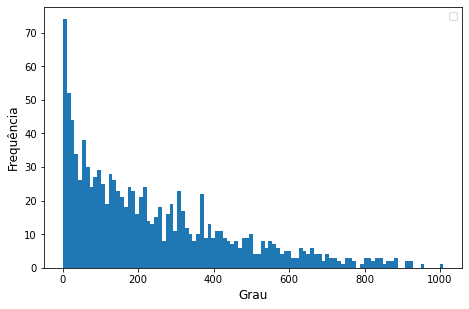
\includegraphics[scale=0.6]{images/base-de-dados-29-degree-distribution-cnae.png}
    \label{fig:metricas-redes:base-de-dados-29-degree-distribution-cnae}
    \fdadospesquisa
\end{figure}

A rede também apresenta uma transitividade significativa que reflete a conectividade da rede e uma tendência leve à desassortatividade de grau. A assortatividade de seção não indicou nenhuma tendência, indicando que não existe preferência dos vértices de se conectarem ou não à vértices da mesma seção.

As Tabelas~\ref{tab:metricas-redes:grafo-por-cnae-especificas1} e \ref{tab:metricas-redes:grafo-por-cnae-especificas2} apresentam a distribuição das outras métricas estudadas. Novamente, foram usadas as formulações utilizando arestas ponderadas para o estudo.

\begin{table}[htb]
\centering
\caption{Métricas do grafo de transações entre CNAEs segmentadas por CNAE (Parte 1)}
\label{tab:metricas-redes:grafo-por-cnae-especificas1}
\begin{tabular}{l|rrrrr}
\toprule
Métrica & Grau & \shortstack{Coeficiente\\de agrupamento} & Excentricidade & \shortstack{Caminho\\mínimo médio} & \shortstack{Caminho mínimo\\médio ponderado} \\
\midrule
Média         &  241.1 &   $1.471e^{-05}$ & 2.917 & 1.8160 & $1.140e^{-05}$ \\
Desvio Padrão &  213.7 &   $1.946e^{-05}$ & 0.309 & 0.2289 & $6.641e^{-05}$ \\
Mínimo        &    1   &                0 &     2 & 1.1030 & $5.708e^{-06}$ \\
25º percentil &   66   &   $4.441e^{-06}$ &     3 & 1.6800 & $5.722e^{-06}$ \\
50º percentil &  183   &   $9.605e^{-06}$ &     3 & 1.8470 & $5.776e^{-06}$ \\
75º percentil &  365   &   $1.790e^{-05}$ &     3 & 1.9640 & $6.351e^{-06}$ \\
Máximo        & 1009   &           0.0003 &     4 & 2.7970 &         0.0019 \\
\bottomrule
\end{tabular}
\fdadospesquisa
\end{table}

\begin{table}[htb]
\centering
\caption{Métricas do grafo de transações entre CNAEs segmentadas por CNAE (Parte 2)}
\label{tab:metricas-redes:grafo-por-cnae-especificas2}
\begin{tabular}{l|rrrrr}
\toprule
Métrica & \shortstack{Centralidade\\de informação} & \shortstack{Centralidade\\de autovalor} & \shortstack{Centralidade de\\intermediação} & \shortstack{Centralidade\\de proximidade} & PageRank \\
\midrule
Média         & 225.9    &         0.0020 &         0.0007 & 0.5598 & 0.0008 \\
Desvio Padrão &  47.49   &         0.0298 &         0.0019 & 0.0769 & 0.0021 \\
Mínimo        &   0.4702 & $3.198e^{-12}$ &              0 & 0.3572 & 0.0001 \\
25º percentil & 235.5    & $3.452e^{-07}$ & $3.047e^{-06}$ & 0.5086 & 0.0001 \\
50º percentil & 245.4    & $5.856e^{-06}$ & $5.415e^{-05}$ & 0.5409 & 0.0002 \\
75º percentil & 246.3    & $7.721e^{-05}$ &         0.0005 & 0.5947 & 0.0007 \\
Máximo        & 246.4     &         0.8161 &         0.0287 & 0.9057 & 0.0316 \\
\bottomrule
\end{tabular}
\fdadospesquisa
\end{table}

Analisando a distribuição do coeficiente de agrupamento, é possível verificar que existe uma certa variância que indicam a presença de alguns vértices com agrupamento local significativo, embora a magnitude da métrica seja bastante influenciada pelo fato de usar a formulação para arestas ponderadas. Por outro lado, a excentricidade dos vértices apresenta pouca variância o que reflete uma rede curta, de baixo diâmetro e raio, da mesma forma que a distribuição do caminho mínimo médio partindo dos vértices também possui uma variância limitada e fortemente correlacionada ao grau.

As métricas de centralidade de informação, de proximidade e de proximidade são novamente influenciadas pelo volume transacionado por cada CNAE e sofrem certo efeito também do baixo comprimento da rede, apresentando uma variância também baixa. Já a centralidade de autovalor e o pagerank apresentam variância significativa possivelmente refletindo o valor total transacionado pelos vértices e não sendo tão influenciados pela topologia da rede.

\subsection{Conclusões}
\label{section:metricas-redes:conclusoes}

Assim, fica claro a partir da caracterização das redes com dados de 2019 que são redes com topologias não tão complexas e que possuem uma forte correlação com os valores transacionados por cada entidade. Apesar disso, este estudo pode adicionar informações importantes sobre a topologia dessas redes que serão usadas no estudo do impacto da pandemia do ponto de vista topológico e podem ser usados para a detecção ou decisão de entidades que tiveram impacto da pandemia.

\section{Alterações topológicas}
\label{section:alteracoes-topologicas}

Nesta seção, vamos analisar mudanças que ocorreram na estrutura das redes para o período da pandemia em comparação com a topologia vista na caracterização anterior.

\subsection{Redes UF-UF}
\label{section:alteracoes-topologicas:uf}

\begin{table}[htb]
\centering
\caption{Variação percentual das métricas de redes mês a mês para o grafo de UFs (Parte 1)}
\label{tab:metricas-redes-pandemia:grafo-mensal-por-uf1}
\begin{tabular}{l|rrrr}
\toprule
Mês & Densidade & Transitividade & Grau médio & \shortstack{Grau médio\\ponderado} \\
\midrule
01/2019 & - & - & - & - \\
02/2019 & +0.54\% & +0.55\% & +0.54\% &  +9.88\% \\
03/2019 & +0.00\% & +0.17\% & +0.00\% & +25.54\% \\
04/2019 & +0.54\% & +0.57\% & +0.54\% & +23.86\% \\
05/2019 & +0.81\% & +0.81\% & +0.81\% & +36.91\% \\
06/2019 & +0.27\% & +0.32\% & +0.27\% & +23.88\% \\
07/2019 & +0.54\% & +0.57\% & +0.54\% & +28.36\% \\
08/2019 & +0.54\% & +0.57\% & +0.54\% & +35.37\% \\
09/2019 & +0.27\% & +0.36\% & +0.27\% & +32.62\% \\
10/2019 & +0.81\% & +0.82\% & +0.81\% & +42.89\% \\
11/2019 & +0.27\% & +0.34\% & +0.27\% & +43.93\% \\
12/2019 & +0.27\% & +0.36\% & +0.27\% & +29.66\% \\
01/2020 & +0.81\% & +0.83\% & +0.81\% & +28.84\% \\
02/2020 & +0.27\% & +0.44\% & +0.27\% & +32.22\% \\
03/2020 & +0.54\% & +0.59\% & +0.54\% & +36.09\% \\
04/2020 & -0.27\% & -0.07\% & -0.27\% &  -7.91\% \\
05/2020 & -0.27\% & -0.18\% & -0.27\% & +12.47\% \\
06/2020 & +0.00\% & +0.11\% & +0.00\% & +34.61\% \\
07/2020 & +0.54\% & +0.57\% & +0.54\% & +62.51\% \\
08/2020 & +0.54\% & +0.59\% & +0.54\% & +55.16\% \\
09/2020 & +1.08\% & +1.09\% & +1.08\% & +60.32\% \\
10/2020 & +0.00\% & +0.17\% & +0.00\% & +61.19\% \\
\bottomrule
\end{tabular}
\fdadospesquisa
\end{table}

Primeiramente, vamos analisar alterações topológicas na estrutura das redes UF-UF no período que compreende janeiro de 2019 e outubro de 2020. Para esta análise, os dados foram dividido mês a mês e um grafo foi criado para cada mês do período estudado. Cada vértice destes grafos representa uma UF e cada aresta representa o valor total transacionado entre duas UFs naquele mês. Usamos novamente a modelagem de grafo cíclico ponderado, sendo que cada aresta possui novamente um atributo indicando a distância entre os vértices igual ao inverso do valor transacionado. Cada vértice possui também um atributo indicando a região a qual pertence aquela UF, usado em uma das métricas de assortatividade.

A Tabelas~\ref{tab:metricas-redes-pandemia:grafo-mensal-por-uf1} e \ref{tab:metricas-redes-pandemia:grafo-mensal-por-uf2} mostram a evolução de algumas métricas gerais das redes UF-UF para cada mês do período analisado. Cada linha da tabela representa o valor da métrica analisada em relação ao mês de janeiro de 2019, mostrando assim a evolução percentual em relação a esse mês-base.

\begin{table}[htb]
\centering
\caption{Variação das métricas de redes mês a mês para o grafo de UFs (Parte 2)}
\label{tab:metricas-redes-pandemia:grafo-mensal-por-uf2}
\begin{tabular}{l|rrrr}
\toprule
Mês & \shortstack{Assortatividade\\de grau} & \shortstack{Assortatividade\\de região} & \shortstack{Caminho mínimo\\médio} & \shortstack{Caminho mínimo\\médio ponderado} \\
\midrule
01/2019 & - & - & - & - \\
02/2019 & -15.60\% & -50.13\% & -0.55\% &  -8.47\% \\
03/2019 &  +0.05\% &  -0.00\% & +0.00\% & -25.12\% \\
04/2019 &  +7.91\% & -15.39\% & -0.55\% & -22.23\% \\
05/2019 & -31.31\% & -85.53\% & -0.83\% & -25.07\% \\
06/2019 & +21.99\% & +13.35\% & -0.27\% &  +2.44\% \\
07/2019 & -17.07\% & -57.33\% & -0.55\% &  -1.69\% \\
08/2019 &  +7.91\% & -57.33\% & -0.55\% & -11.02\% \\
09/2019 &  +4.73\% & -28.82\% & -0.27\% &  -2.55\% \\
10/2019 &  -6.87\% & -43.83\% & -0.83\% & -11.15\% \\
11/2019 &  +8.56\% & +13.35\% & -0.27\% & -14.48\% \\
12/2019 &  +4.73\% & -70.86\% & -0.27\% &  +2.50\% \\
01/2020 & -25.43\% & -43.83\% & -0.83\% &  +1.69\% \\
02/2020 & -18.97\% & -28.82\% & -0.27\% &  -5.58\% \\
03/2020 &  -7.22\% & -15.39\% & -0.55\% &  -4.69\% \\
04/2020 &  +1.98\% & -13.38\% & +0.27\% & +36.70\% \\
05/2020 & +37.79\% & +29.14\% & +0.27\% &  +2.72\% \\
06/2020 & +19.66\% & -42.28\% & +0.00\% & -15.66\% \\
07/2020 &  +7.91\% & -15.39\% & -0.55\% & -32.97\% \\
08/2020 &  -7.22\% & -15.39\% & -0.55\% & -35.56\% \\
09/2020 & -16.88\% & -71.96\% & -1.11\% & -37.64\% \\
10/2020 &  +0.05\% & -42.28\% &  0.00\% & -30.06\% \\
\bottomrule
\end{tabular}
\fdadospesquisa
\end{table}

A partir desses dados, é possível ver que as oscilações mês a mês nas métricas são pequenas, muitas vezes menor que 1\%. Quando analisamos as densidade, transitividade, e grau médio, podemos ver que nos meses de abril e maio de 2020 há uma queda pequena mas consistente em todas essas métricas. Isso mostra uma pequena perda de de conectividade geral da rede, que se recupera e retoma os níveis anteriores a partir de agosto de 2020. Analisando o grau médio ponderado, uma métrica que envolve valores transacionados, podemos ver que a variância nos meses anteriores à crise é maior, em patamares de dezenas de pontos percentuais, e da mesma forma o impacto da crise nos meses de abril e maio é mais significativo, chegando a ser 7\% menor que o mês-base.

Analisando a assortatividade de grau e de região, podemos notar também uma variância mais significativa a partir dos dados nos meses que precedem a pandemia. Não há uma tendência clara em nenhuma dessas métricas, sendo que elas oscilam positivamente e negativamente no decorrer do tempo e não podemos deduzir que a variação para os meses de maior impacto da pandemia tem relação com a crise. No mês de maio, há um aumento pontual de ambas assortatividades, mas logo retornando às variações e aos patamares anteriores nos meses seguintes.

Ao observar o caminho mínimo médio verificamos uma variância pequena nos meses que precedem a pandemia, tendendo a encurtar os caminhos mínimos em relação ao mês-base, e nos meses do segundo trimestre de 2020 há um aumento tímido mas consistente desta métrica, voltando aos patamares anteriores após esse período. Utilizando a análise de caminhos mínimos ponderados observamos uma variação maior dos dados, novamente com tendência de diminuição da métrica nos meses que precedem a pandemia em relação ao mês base, sendo que nos meses de abril e maio a métrica tem um aumento consideravelmente consistente e depois alcança um patamar de alta diminuição dos caminhos mínimos em relação ao mês-base.

\begin{table}[htb]
\centering
\caption{Variação das métricas de rede a cada trimestre para o grafo de UFs (Parte 1)}
\label{tab:metricas-redes-pandemia:grafo-trimestral-por-uf1}
\begin{tabular}{l|rrrr}
\toprule
Mês & Densidade & Transitividade & Grau médio & \shortstack{Grau médio\\ponderado} \\
\midrule
2020/1 & - & - & - & - \\
2020/2 & -0.80\% & -0.78\% & -0.80\% & -14.60\% \\
2020/3 & +0.27\% & +0.22\% & +0.27\% & +20.35\% \\
\bottomrule
\end{tabular}
\fdadospesquisa
\end{table}

\begin{table}[htb]
\centering
\caption{Variação das métricas de rede a cada trimestre para o grafo de UFs (Parte 2)}
\label{tab:metricas-redes-pandemia:grafo-trimestral-por-uf2}
\begin{tabular}{l|rrrr}
\toprule
Mês & \shortstack{Assortatividade\\de grau} & \shortstack{Assortatividade\\de região} & \shortstack{Caminho mínimo\\médio} & \shortstack{Caminho mínimo\\médio ponderado} \\
\midrule
2020/1 & - & - & - & - \\
2020/2 & +77.29\% &  +1.84\% & +0.85\% &  +6.63\% \\
2020/3 & -34.35\% & -83.36\% & -0.28\% & -33.74\% \\
\bottomrule
\end{tabular}
\fdadospesquisa
\end{table}

É possível traçar uma relação entre a diminuição da conectividade e o aumento dos caminhos mínimos, uma vez que tais métricas são naturalmente inversamente proporcionais: quanto mais conectado é uma rede, menor são os caminhos mínimos necessários para percorrê-la. Isso não significa necessariamente uma relação causal, uma vez que a perda de conectividade da rede foi aparentemente bastante pequena, apesar de consistente.

Por fim, analisamos as Tabelas~\ref{tab:metricas-redes-pandemia:grafo-trimestral-por-uf1} e \ref{tab:metricas-redes-pandemia:grafo-trimestral-por-uf2} que repetem a mesma análise, mas agora com grafos utilizando dados trimestrais ao invés de mensais. São mantidas as mesmas regras de formação dos grafos conforme a descrição anterior. A análise agora passa a ser em relação ao primeiro trimestre de 2020, que tomamos como trimestre-base.

Novamente, é possível observar perda de conectividade na rede em pequenos mas consistentes percentuais, afetando as métricas densidade, transitividade, grau médio, e grau médio ponderado. Essa conectividade é aparentemente recuperada no trimestre posterior. Por outro lado, as redes apresentam um ganho significativo de assortatividade de grau, indicando preferência dos vértices de se conectar a vértices semelhantes. A assortatividade de região e as métricas de caminhos mínimos médios apresentaram tímido aumento percentual. Essas outras métricas tiveram queda no trimestre seguinte, em sentido contrário ao apresentado.

% \begin{table}[htb]
% \centering
% \caption{Diferença entre as métricas de rede para UFs afetadas e não afetadas}
% \label{tab:metricas-redes-pandemia:diferenca-afetadas-por-uf}
% \begin{tabular}{l|rrrrrrr}
% \toprule
% Métrica & Média & \shortstack{Desvio\\padrão} & Mínimo & P25 & Mediana & P75 & Máximo \\
% \midrule
% Grau médio                     & -1.85\% &   +2.51\% &  -0.26\% & -3.70\% &  +0.00\% &  +0.00\% &    +0.00\% \\ \hline
% \shortstack[l]{Coeficiente de\\agrupamento}     &  +0.33\% &   +4.71\% &   +2.79\% & -2.34\% & -0.83\% &  6.67\% &  -14.51\% \\ \hline
% Excentricidade                 & -4.17\% & -20.41\% &   +0.00\% &  +0.00\% &  +0.00\% &  +0.00\% & -100.00\% \\ \hline
% \shortstack[l]{Caminho mínimo\\médio}           &  +1.85\% &   +2.46\% &   +0.00\% &  +0.00\% &  +0.00\% &  +3.70\% &   -0.28\% \\ \hline
% \shortstack[l]{Caminho mínimo\\médio ponderado} & -6.58\% &   +0.14\% &  -2.01\% & -7.36\% & -0.36\% & -1.03\% &  -37.83\% \\ \hline
% \shortstack[l]{Centralidade de\\proximidade}    & -1.71\% &   +2.28\% &   +0.25\% & -3.45\% &  +0.00\% &  +0.00\% &    +0.00\% \\ \hline
% \shortstack[l]{Centralidade de\\informação}     & -1.07\% &  -1.71\% &   +9.93\% & -1.09\% &  +0.16\% &  +0.10\% &   -8.60\% \\ \hline
% \shortstack[l]{Centralidade de\\autovalor}      & -3.84\% &  -1.85\% &  +23.00\% & -0.99\% & -1.58\% & -4.25\% &  -20.99\% \\ \hline
% \shortstack[l]{Centralidade de\\intermediação}  &  - &     - & 206.06\% &  +0.00\% &  +0.00\% &  +0.00\% &    - \\ \hline
% PageRank                       & -0.63\% &   +0.02\% &   +4.37\% & -1.23\% & -1.61\% & -1.01\% &   -5.26\% \\
% \bottomrule
% \end{tabular}
% \fdadospesquisa
% \end{table}

\subsection{Redes Seção-Seção}
\label{section:alteracoes-topologicas:secao}

\begin{table}[htb]
\centering
\caption{Variação percentual das métricas de redes mês a mês para o grafo de seções (Parte 1)}
\label{tab:metricas-redes-pandemia:grafo-mensal-por-secao1}
\begin{tabular}{l|rrrr}
\toprule
Mês & Densidade & Transitividade & Grau médio & \shortstack{Grau médio\\ponderado} \\
\midrule
01/2019 &  - &  - &  - &  - \\
02/2019 & -0.57\% & -0.55\% & -0.57\% &  +9.89\%\\
03/2019 & +0.57\% & +0.31\% & +0.57\% & +25.54\%\\
04/2019 & -1.15\% & -1.20\% & -1.15\% & +23.86\%\\
05/2019 & +1.15\% & +0.15\% & +1.15\% & +36.92\%\\
06/2019 & -1.72\% & -1.33\% & -1.72\% & +23.89\%\\
07/2019 & -0.57\% & -1.00\% & -0.57\% & +28.37\%\\
08/2019 & -0.57\% & -0.63\% & -0.57\% & +35.37\%\\
09/2019 & +0.00\% & +0.18\% & +0.00\% & +32.63\%\\
10/2019 & -0.57\% & +0.13\% & -0.57\% & +42.89\%\\
11/2019 & -1.72\% & -1.25\% & -1.72\% & +43.94\%\\
12/2019 & +1.15\% & +0.85\% & +1.15\% & +29.66\%\\
01/2020 & +2.30\% & +1.87\% & +2.30\% & +28.85\%\\
02/2020 & +1.15\% & +0.46\% & +1.15\% & +32.22\%\\
03/2020 & +1.72\% & +0.98\% & +1.72\% & +36.10\%\\
04/2020 & -0.57\% & -0.38\% & -0.57\% &  -7.92\%\\
05/2020 & -0.57\% & -0.47\% & -0.57\% & +12.47\%\\
06/2020 & -1.72\% & -0.72\% & -1.72\% & +34.62\%\\
07/2020 & -1.72\% & -1.97\% & -1.72\% & +62.52\%\\
08/2020 & +0.00\% & -0.15\% & +0.00\% & +55.16\%\\
09/2020 & +1.72\% & +1.24\% & +1.72\% & +60.33\%\\
10/2020 & +0.00\% & -0.60\% & +0.00\% & +61.20\%\\
\bottomrule
\end{tabular}
\fdadospesquisa
\end{table}

A seguir, serão analisadas alterações topológicas na estrutura das redes Seção-Seção no período que compreende janeiro de 2019 e outubro de 2020. Nesta análise, os dados foram mais uma vez dividido mês a mês e um grafo foi criado para cada mês do período estudado. Cada vértice destes grafos representa uma seção e cada aresta representa o valor total transacionado entre duas seções naquele mês. Usamos novamente a modelagem de grafo cíclico ponderado, sendo que cada aresta possui novamente um atributo indicando a distância entre os vértices igual ao inverso do valor transacionado.

As Tabelas~\ref{tab:metricas-redes-pandemia:grafo-mensal-por-secao1} e \ref{tab:metricas-redes-pandemia:grafo-mensal-por-secao2} apresentam a evolução das métricas das redes Seção-Seção para cada mês. Cada linha mostra portanto a variação do valor das métricas do grafo montado para aquele mês em relação ao mês de janeiro de 2019, usado novamente como mês-base.

Assim como nas redes UF-UF, temos aqui uma baixa variação nos dados das métricas de densidade, transitividade, e grau médio, sendo que a magnitude da variação dessas métricas é menor que 2.5\%, o que dificulta afirmações mais assertivas. Para essas três métricas, não existe uma tendência clara de crescimento ou redução de cada métrica no decorrer do tempo, sendo que comparando os meses imediatamente anteriores à crise com os meses mais críticos (abril e maio de 2020), há uma aparente queda de densidade e transitividade indicando uma leve redução na conectividade da rede, que apresenta evolução nos meses seguintes. Quando observamos o grau médio ponderado, uma métrica influenciada pelo volume mensal de transações, podemos então ver que nos meses mais críticos da crise o grau médio diminuiu, indicando um menor fluxo de transações entre os vértices das redes.

Ao analisar a assortatividade de grau podemos ver uma variação nessas métricas sem tendência clara de crescimento ou redução para todo o período analisado. A métrica caminho mínimo médio também apresenta uma variação sem tendência clara e com baixa magnitude, com uma leve alta nos meses mais críticos da crise em relação aos meses imediatamente anteriores, mas não sendo o suficiente para indicar uma tendência. Quando analisamos o grau médio ponderado por outro lado, métrica influenciada pelo volume de transações, podemos verificar que nos meses de abril e maio de 2020 há uma variação significativa que indica aumento desta métrica em relação aos meses imediatamente anteriores e posteriores.

As Tabelas~\ref{tab:metricas-redes-pandemia:grafo-trimestral-por-secao1} e \ref{tab:metricas-redes-pandemia:grafo-trimestral-por-secao2} mostram a mesma análise mas do ponto de vista trimestral em relação ao primeiro trimestre de 2020, tomado como trimestre-base.

\begin{table}[htb]
\centering
\caption{Variação das métricas de redes mês a mês para o grafo de seções (Parte 2)}
\label{tab:metricas-redes-pandemia:grafo-mensal-por-secao2}
\begin{tabular}{l|rrrr}
\toprule
Mês & \shortstack{Assortatividade\\de grau} & \shortstack{Caminho mínimo\\médio} & \shortstack{Caminho mínimo\\médio ponderado} \\
\midrule
01/2019 &  - &  - &  - \\
02/2019 &  +2.76\% & +0.45\% & +29.22\% \\
03/2019 &  -9.42\% & -0.45\% & -11.35\% \\
04/2019 &  +4.86\% & +0.90\% &  +2.19\% \\
05/2019 &  +1.47\% & -0.45\% &  +3.75\% \\
06/2019 & +16.41\% & +0.90\% &  +5.20\% \\
07/2019 &  +1.48\% & +0.45\% & -15.91\% \\
08/2019 &  +6.16\% & +0.45\% & -13.54\% \\
09/2019 &  -5.13\% & -0.45\% & -10.76\% \\
10/2019 &  -1.58\% & +0.00\% & -15.12\% \\
11/2019 &  10.43\% & +0.90\% & -38.71\% \\
12/2019 &  -3.53\% & -0.90\% & -41.20\% \\
01/2020 & -14.48\% & -1.80\% & -25.39\% \\
02/2020 &  -1.24\% & -0.45\% & -36.64\% \\
03/2020 &  -7.40\% & -0.90\% & +22.58\% \\
04/2020 &  -4.91\% & +0.45\% & +28.02\% \\
05/2020 &  -8.57\% & +0.45\% & +114.33\% \\
06/2020 &  -3.99\% & +1.35\% & +72.81\% \\
07/2020 &  -4.68\% & +1.80\% & +65.47\% \\
08/2020 & -11.69\% & +0.45\% & +60.28\% \\
09/2020 & -10.17\% & -0.90\% & +56.97\% \\
10/2020 &  -6.61\% & +0.45\% & -33.58\% \\
\bottomrule
\end{tabular}
\fdadospesquisa
\end{table}

Ao observarmos agora de forma agregada os dados trimestrais de 2020, podemos ver pela densidade, transitividade, e grau médio que há uma leve redução na conectividade da rede nos trimestres após o começo da pandemia em relação ao trimestre-base. Quando incluímos o grau médio ponderado, vemos que há uma queda significativa no segundo trimestre em relação ao trimestre-base e que há recuperação no trimestre seguinte.

A seguir, verificamos uma tendência de alta da assortatividade de grau durante o trimestre mais crítico da crise, retornando ao patamar anterior no trimestre seguinte. E ao analisar o caminho mínimo médio podemos ver que não há variação significativa em relação ao trimestre-base, mas quando fazemos a análise da métrica ponderada é possível verificar um aumento considerável no distância entre os vértices da rede.

\begin{table}[htb]
\centering
\caption{Variação das métricas de rede a cada trimestre para o grafo de seções (Parte 1)}
\label{tab:metricas-redes-pandemia:grafo-trimestral-por-secao1}
\begin{tabular}{l|rrrr}
\toprule
Mês & Densidade & Transitividade & Grau médio & \shortstack{Grau médio\\ponderado} \\
\midrule
2020/1 & - & - & - & - \\
2020/2 & -1.66\% & -0.92\% & -1.66\% & -14.60\% \\
2020/3 & -1.10\% & -0.59\% & -1.10\% & +20.35\% \\
\bottomrule
\end{tabular}
\fdadospesquisa
\end{table}

\begin{table}[htb]
\centering
\caption{Variação das métricas de rede a cada trimestre para o grafo de seções (Parte 2)}
\label{tab:metricas-redes-pandemia:grafo-trimestral-por-secao2}
\begin{tabular}{l|rrrr}
\toprule
Mês & \shortstack{Assortatividade\\de grau} & \shortstack{Caminho mínimo\\médio} & \shortstack{Caminho mínimo\\médio ponderado} \\
\midrule
2020/1 & - & - & - & - \\
2020/2 & +11.16\% & +0.93\% & +122.98\% \\
2020/3 &  -2.87\% & +0.93\% & +100.19\% \\
\bottomrule
\end{tabular}
\fdadospesquisa
\end{table}

% \begin{table}[htb]
% \centering
% \caption{Diferença entre as métricas de rede para seções afetadas e não afetadas}
% \label{tab:metricas-redes-pandemia:diferenca-afetadas-por-secao}
% \begin{tabular}{l|rrrrrrr}
% \toprule
% Métrica & Média & \shortstack{Desvio\\padrão} & Mínimo & P25 & Mediana & P75 & Máximo \\
% \midrule
% Grau médio                     &  +0.02\% & -0.04\% & +0.11\% & +0.05\% &  +0.00\% &  +0.00\% & -0.05\% \\ \hline
% \shortstack[l]{Coeficiente de\\agrupamento}     &  +0.16\% & -0.01\% & +0.38\% & +0.15\% &  +0.11\% &  +0.14\% &  +0.07\% \\ \hline
% Excentricidade                 &  +0.00\% &  +0.00\% & +0.00\% & +0.00\% &  +0.00\% &  +0.00\% &  +0.00\% \\ \hline
% \shortstack[l]{Caminho mínimo\\médio}           & -0.01\% & -0.03\% & +0.05\% & +0.00\% &  +0.00\% & -0.04\% & -0.05\% \\ \hline
% \shortstack[l]{Caminho mínimo\\médio ponderado} &  +0.00\% & -0.00\% & +0.00\% & +0.00\% & -0.00\% & -0.00\% & -0.00\% \\ \hline
% \shortstack[l]{Centralidade de\\proximidade}    &  +0.01\% & -0.03\% & +0.05\% & +0.04\% &  +0.00\% &  +0.00\% & -0.05\% \\ \hline
% \shortstack[l]{Centralidade de\\informação}     &  +0.00\% & -0.00\% & +0.00\% & +0.00\% &  +0.00\% & -0.00\% & -0.00\% \\ \hline
% \shortstack[l]{Centralidade de\\autovalor}      &  +0.32\% & -0.00\% & +0.56\% & +0.39\% &  +0.20\% &  +0.25\% &  +0.28\% \\ \hline
% \shortstack[l]{Centralidade de\\intermediação}  &  +0.43\% &  +0.12\% & +0.76\% & +0.34\% &  +0.00\% &  +0.46\% &  +0.00\% \\ \hline
% PageRank                       &  +0.07\% & -0.04\% & +0.17\% & +0.07\% &  +0.08\% &  +0.11\% & -0.21\% \\
% \bottomrule
% \end{tabular}
% \fdadospesquisa
% \end{table}

\subsection{Redes CNAE-CNAE}
\label{section:alteracoes-topologicas:cnae}

Por fim, serão apresentadas as alterações topológicas na estrutura das redes CNAE-CNAE no período que compreende janeiro de 2019 e outubro de 2020.

\begin{table}[htb]
\centering
\caption{Variação percentual das métricas de redes mês a mês para o grafo de CNAEs (Parte 1)}
\label{tab:metricas-redes-pandemia:grafo-mensal-por-cnae1}
\begin{tabular}{l|rrrr}
\toprule
Mês & Densidade & Transitividade & Grau médio & \shortstack{Grau médio\\ponderado} \\
\midrule
01/2019 & - & - & - & - \\
02/2019 &  +4.35\% &  +1.75\% &  +4.45\% &  +9.79\% \\
03/2019 &  +5.96\% &  +2.29\% &  +6.15\% & +25.32\% \\
04/2019 &  +9.60\% &  +3.67\% &  +9.70\% & +23.75\% \\
05/2019 & +11.46\% &  +4.22\% & +11.66\% & +36.67\% \\
06/2019 &  +7.55\% &  +2.71\% &  +7.55\% & +23.89\% \\
07/2019 & +12.16\% &  +4.16\% & +12.06\% & +28.48\% \\
08/2019 & +12.70\% &  +4.64\% & +12.80\% & +35.25\% \\
09/2019 & +11.38\% &  +4.45\% & +11.48\% & +32.51\% \\
10/2019 & +13.87\% &  +5.36\% & +14.27\% & +42.38\% \\
11/2019 & +12.57\% &  +4.84\% & +12.67\% & +43.81\% \\
12/2019 &  +6.15\% &  +2.35\% &  +6.62\% & +29.09\% \\
01/2020 &  +9.87\% &  +3.64\% & +10.27\% & +28.39\% \\
02/2020 &  +8.58\% &  +3.01\% &  +8.87\% & +31.87\% \\
03/2020 &  +9.29\% &  +3.80\% &  +9.68\% & +35.62\% \\
04/2020 &  -2.40\% &  -0.24\% &  -2.40\% &  -7.92\% \\
05/2020 &  +1.98\% &  +1.67\% &  +2.07\% & +12.37\% \\
06/2020 &  +7.94\% &  +3.99\% &  +8.13\% & +34.38\% \\
07/2020 & +11.86\% &  +5.21\% & +12.46\% & +61.65\% \\
08/2020 & +10.99\% &  +4.48\% & +10.89\% & +55.30\% \\
09/2020 &  +9.68\% &  +4.69\% & +10.26\% & +59.47\% \\
10/2020 &  +7.63\% &  +3.96\% &  +8.02\% & +60.62\% \\
\bottomrule
\end{tabular}
\fdadospesquisa
\end{table}

Da mesma forma, os dados foram dividido mês a mês e um grafo foi criado para cada mês do período estudado. Cada vértice destes grafos representa um CNAE e cada aresta representa o valor total transacionado entre dois CNAEs naquele mês. Usamos novamente a modelagem de grafo cíclico ponderado, sendo que cada aresta possui novamente um atributo indicando a distância entre os vértices igual ao inverso do valor transacionado. Cada vértice possui também um atributo indicando a seção a que pertence aquele CNAE para uso na métrica de assortatividade.

As Tabelas~\ref{tab:metricas-redes-pandemia:grafo-mensal-por-cnae1} e \ref{tab:metricas-redes-pandemia:grafo-mensal-por-cnae2} apresentam as métricas desta análise, apresentando a variação percentual de cada métrica para cada mês em relação ao mês-base de janeiro de 2019.

\begin{table}[htb]
\centering
\caption{Variação das métricas de redes mês a mês para o grafo de CNAEs (Parte 2)}
\label{tab:metricas-redes-pandemia:grafo-mensal-por-cnae2}
\begin{tabular}{l|rrrr}
\toprule
Mês & \shortstack{Assortatividade\\de grau} & \shortstack{Assortatividade\\de seção} & \shortstack{Caminho mínimo\\médio} & \shortstack{Caminho mínimo\\médio ponderado} \\
\midrule
01/2019 & - & - & - & - \\
02/2019 &  +0.38\% &  -6.76\% & -0.72\% &  -9.37\% \\
03/2019 &  +1.52\% & -22.04\% & -0.93\% & +35.22\% \\
04/2019 &  +1.80\% &  -8.60\% & -1.49\% & +33.50\% \\
05/2019 &  +2.69\% & -23.49\% & -1.83\% & -13.22\% \\
06/2019 &  +1.02\% & -24.50\% & -1.15\% & -15.84\% \\
07/2019 &  +1.76\% &  +4.38\% & -1.77\% & -17.73\% \\
08/2019 &  +1.77\% & -16.28\% & -1.64\% &  +3.81\% \\
09/2019 &  +0.86\% &  +3.95\% & -1.65\% & -29.89\% \\
10/2019 &  +1.55\% &  -4.69\% & -1.83\% & -35.86\% \\
11/2019 &  +1.02\% &  -8.01\% & -1.83\% & -36.74\% \\
12/2019 &  +0.52\% & -10.46\% & -1.08\% & -30.56\% \\
01/2020 &  +2.06\% &  -6.52\% & -1.50\% & -28.02\% \\
02/2020 &  +1.27\% &  +9.35\% & -1.30\% & -23.95\% \\
03/2020 &  +1.61\% &  +1.73\% & -1.40\% & -23.14\% \\
04/2020 &  -0.02\% &  +8.10\% & +0.58\% &  -8.54\% \\
05/2020 &  +1.14\% & +16.10\% & -0.27\% &  +9.73\% \\
06/2020 &  +2.35\% &  +0.88\% & -1.13\% & +16.51\% \\
07/2020 &  +3.60\% & +15.25\% & -1.66\% &  +1.86\% \\
08/2020 &  +1.83\% & +12.58\% & -1.57\% & -26.79\% \\
09/2020 &  +2.24\% & +16.47\% & -1.21\% &  +5.56\% \\
10/2020 &  +1.30\% &  -4.01\% & -0.98\% & -17.64\% \\
\bottomrule
\end{tabular}
\fdadospesquisa
\end{table}

Mais uma vez, podemos verificar a redução da conectividade das redes através da densidade, da transitividade e do grau médio da rede em relação ao mês-base, com as três métricas apresentando redução em relação aos meses imediatamente anteriores ao início da crise e se recuperando nos meses posteriores aos meses mais críticos. Essa métricas agora apresentam uma variação de magnitude significativa, sendo mais importante que nas redes analisadas anteriormente. Se considerarmos o grau médio ponderado essa diferença se torna ainda mais significativa, também com tendência de redução durante os meses mais críticos e posterior recuperação.

Analisando a assortatividade de grau das redes, é possível ver que existe pouca variação em relação ao mês-base, e que no mês de abril de 2020 há uma variação diferente para leve disassortatividade, voltando para os patamares anteriores nos meses seguintes. Já quando observamos a assortatividade de seção, vemos uma variação de magnitude mais significativa, e que apresenta tendência positiva nos meses da pandemia que se mantém até setembro de 2020. Essa tendência de aumento na assortatividade de seção é interessante pois indicaria que na rede de CNAEs as seções tem alguma preferência de se conectar com seções semelhantes.

Por fim, analisando o caminho mínimo médio, é possível verificar certa estabilidade no período analisado em relação ao mês-base, com exceção dos meses de abril de maio de 2020 quando aparentemente há um aumento da distância entre os vértices das redes. Quando incluímos ponderação pelo valor transacionado na análise, essa diferença se torna ainda mais evidente, com uma alta que impacta também meses posteriores aos meses mais críticos.

\begin{table}[htb]
\centering
\caption{Variação das métricas de rede a cada trimestre para o grafo de CNAEs (Parte 1)}
\label{tab:metricas-redes-pandemia:grafo-trimestral-por-cnae1}
\begin{tabular}{l|rrrr}
\toprule
Mês & Densidade & Transitividade & Grau médio & \shortstack{Grau médio\\ponderado} \\
\midrule
2020/1 & - & - & - & - \\
2020/2 & -4.91\% & -1.09\% & -4.91\% & -14.60\% \\
2020/3 & +0.82\% & +0.98\% & +0.91\% & +20.25\% \\
\bottomrule
\end{tabular}
\fdadospesquisa
\end{table}

\begin{table}[htb]
\centering
\caption{Variação das métricas de rede a cada trimestre para o grafo de CNAEs (Parte 2)}
\label{tab:metricas-redes-pandemia:grafo-trimestral-por-cnae2}
\begin{tabular}{l|rrrr}
\toprule
Mês & \shortstack{Assortatividade\\de grau} & \shortstack{Assortatividade\\de seção} & \shortstack{Caminho mínimo\\médio} & \shortstack{Caminho mínimo\\médio ponderado} \\
\midrule
2020/1 & - & - & - & - \\
2020/2 & -0.21\% & +8.07\% & +0.98\% & +71.35\% \\
2020/3 & +0.66\% & +3.81\% & +0.05\% & +26.02\% \\
\bottomrule
\end{tabular}
\fdadospesquisa
\end{table}

As Tabelas~\ref{tab:metricas-redes-pandemia:grafo-trimestral-por-cnae1} e \ref{tab:metricas-redes-pandemia:grafo-trimestral-por-cnae2} complementam a análise anterior fazendo novamente a análise agora agregando os dados em trimestres e mostrando a variação em relação ao primeiro trimestre de 2020, o trimestre-base.

Novamente, podemos verificar a perda de conectividade da rede no trimestre mais crítico, o segundo de 2020, com uma redução na densidade, transitividade, e grau médio da rede, apresentando uma retomada no trimestre seguinte. Incluindo o grau médio ponderado, novamente essa variação se mostra mais evidente.

Por fim, analisando a variação das métricas de assortatividade, a assortatividade de grau apresenta leve redução no trimestre mais crítico seguida de leve retomada no trimestre seguinte. A assortatividade de seção apresenta alta no trimestre mais crítico e regularização no trimestre seguinte. A distância entre os vértices medida através do caminho mínimo médio apresenta leve tendência de alta nos trimestres da pandemia e se acentuam quando usamos a análise da métrica ponderada.

% \begin{table}[htb]
% \centering
% \caption{Diferença entre as métricas de rede para CNAEs afetadas e não afetadas}
% \label{tab:metricas-redes-pandemia:diferenca-afetadas-por-cnae}
% \begin{tabular}{l|rrrrrrr}
% \toprule
% Métrica & Média & \shortstack{Desvio\\padrão} & Mínimo & P25 & Mediana & P75 & Máximo \\
% \midrule
% Grau médio                     &  0.02\% & -0.04\% & 0.11\% & 0.05\% &  0.00\% &  0.00\% & -0.05\% \\ \hline
% \shortstack[l]{Coeficiente de\\agrupamento}     &  0.16\% & -0.01\% & 0.38\% & 0.15\% &  0.11\% &  0.14\% &  0.07\% \\ \hline
% Excentricidade                 &  0.00\% &  0.00\% & 0.00\% & 0.00\% &  0.00\% &  0.00\% &  0.00\% \\ \hline
% \shortstack[l]{Caminho mínimo\\médio}           & -0.01\% & -0.03\% & 0.05\% & 0.00\% &  0.00\% & -0.04\% & -0.05\% \\ \hline
% \shortstack[l]{Caminho mínimo\\médio ponderado} &  0.00\% & -0.00\% & 0.00\% & 0.00\% & -0.00\% & -0.00\% & -0.00\% \\ \hline
% \shortstack[l]{Centralidade de\\proximidade}    &  0.01\% & -0.03\% & 0.05\% & 0.04\% &  0.00\% &  0.00\% & -0.05\% \\ \hline
% \shortstack[l]{Centralidade de\\informação}     &  0.00\% & -0.00\% & 0.00\% & 0.00\% &  0.00\% & -0.00\% & -0.00\% \\ \hline
% \shortstack[l]{Centralidade de\\autovalor}      &  0.32\% & -0.00\% & 0.56\% & 0.39\% &  0.20\% &  0.25\% &  0.28\% \\ \hline
% \shortstack[l]{Centralidade de\\intermediação}  &  0.43\% &  0.12\% & 0.76\% & 0.34\% &  0.00\% &  0.46\% &  0.00\% \\ \hline
% PageRank                       &  0.07\% & -0.04\% & 0.17\% & 0.07\% &  0.08\% &  0.11\% & -0.21\% \\
% \bottomrule
% \end{tabular}
% \fdadospesquisa
% \end{table}

\subsection{Conclusões}
\label{section:alteracoes-topologicas:conclusoes}

Nesta seção, fizemos uma descrição da oscilação de diversas métricas de redes através e uma modelagem temporal, comparando com as redes se comportam através do tempo e eventuais tendências.

Para o estudo das redes de topologia mais simples, UF-UF e Seção-Seção, a variação das métricas apresentou uma variação de baixa magnitude, muitas vezes menor que 1\%, mas puderam apresentar algumas tendências consistentes mesmo assim. Pudemos ver que mesmo nessas redes há uma perda de conectividade das redes, principalmente nos meses e trimestres mais críticos, evidenciada quando levamos em consideração as formulações que levam em conta os valores transacionados.

As redes CNAE-CNAE que tem uma topologia mais complexa apresentaram a mesma tendência mas de forma mais significativa, sendo que pudemos observar uma magnitude maior nas variações de cada métricas, refletindo da mesma a perda de conectividade da rede.

A perda de conectividade é um sintoma citado nos trabalhos descritos na seção~\ref{introducao:crise-economica}, que analisam dados de áreas significativamente diferentes, como o transporte aéreo global. Assim como o trabalho citado sobre a correlação do impacto da pandemia no mercado de ações apontava para um aumento do caminho mínimo médio, uma tendência também encontrada neste trabalho.

\section{Detecção de impacto econômico}
\label{section:deteccao-impacto}

Nesta seção, nas últimas seções pudemos verificar como a base de dados analisada se comportou durante a pandemia, sob diferentes perspectivas. Agora vamos apresentar os métodos tentados para a detecção e classificação de impacto econômico, visando tentar identificar de forma automatizada entidades afetadas pela crise sob diferentes modelagens. Todos os conjuntos de dados a seguir foram normalizados utilizando norma euclideana, ou norma L2.

\subsection{Dados de UFs}
\label{section:deteccao-impacto:uf}

Para esta análise, criamos uma matriz foram reunidos os dados descritos na seção~\ref{section:metricas-redes:uf}, as métricas de caracterização da rede UF-UF, com algumas métricas relacionadas ao volume transacionado por cada UF: volume total, quantidade de transações, e valor médio de cada transação. Assim, foi criada uma matriz onde cada linha representa uma UF e cada coluna o valor de uma das métricas de redes ou de transações, totalizando onze variáveis.

Também foi uma criada uma segunda tabela com o impacto mensal e total para cada UF, conforme descrito na seção~\ref{section:impacto:cenario-regional}. O objetivo aqui é observar o comportamento de classificadores ao tentar decidir a partir dos dados das métricas obtidas se é possível classificar uma UF como impactada ou não.

\begin{figure}[htb]
	\centering
    \caption{Percentual de variância explicada de cada componente principal para dados de UFs}
    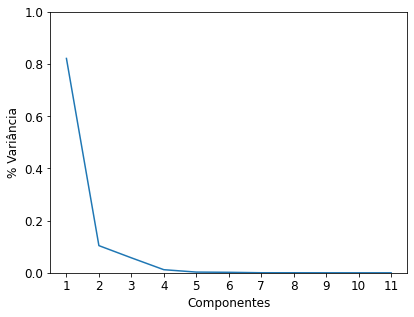
\includegraphics[scale=0.7]{images/base-de-dados-24.1-pca-components-monthly-uf.png}
    \label{fig:resultados:base-de-dados-24-pca-monthly-uf}
    \fdadospesquisa
\end{figure}

Foi feita uma análise de componentes principais a partir dos dados. A Figura~\ref{fig:resultados:base-de-dados-24-pca-monthly-uf} ilustra o percentual da variância explicada pelo conjunto de dados explicada por cada componente principal. As duas primeiras componentes principais concentram a maior parte da variância explicada pelo conjunto de dados.

\begin{table}[htb]
\centering
\caption{Direção de cada métrica em relação a cada uma das duas componentes principais}
\label{tab:resultados:direcao-components-uf}
\begin{tabular}{l|rrrr}
\toprule
Componente & 1 & 2 \\
\midrule
Valor total                    &  0.4746 &  0.1108 \\
Quantidade de transações       &  0.4708 &  0.1544 \\
Valor médio por transação      & -0.0077 & -0.3831 \\
Grau                           &  0.0009 & -0.0101 \\
Coeficiente de agrupamento     &  0.3311 & -0.2535 \\
Excentricidade                 & -0.0226 &  0.2543 \\
Caminho mínimo médio           & -0.0010 &  0.0108 \\
Caminho mínimo médio ponderado & -0.1081 &  0.7227 \\
Centralidade de informação     &  0.0976 & -0.3850 \\
Centralidade de autovalores    &  0.4783 &  0.1268 \\
PageRank                       &  0.4392 &  0.0377 \\
\bottomrule
\end{tabular}
\fdadospesquisa
\end{table}

Na Tabela~\ref{tab:resultados:direcao-components-uf} são descritas as direções de cada variável em relação à cada uma das duas componentes principais. Para a primeira componente se destacam a magnitude do valor total e da quantidade de transações, além da centralidade de autovalores e de informação, enquanto para a segunda componente se destacam o valor médio por transação e novamente a centralidade de informação. As variáveis com maior magnitude terão maior impacto decisivo nos classificadores que usaremos posteriormente.

As Figuras~\ref{fig:resultados:base-de-dados-24.2-pca-2d-monthly-uf} e \ref{fig:resultados:base-de-dados-25.2-pca-2d-total-uf} ilustram a projeção dos dados em relação às duas componentes principais para dar uma noção do espalhamento dos dados, em relação respectivamente ao impacto mensal e impacto total.

\begin{figure}[htb] 
    \centering 
    \caption{Visualização dos dados de UFs projetados sobre as duas componentes principais}
    \label{fig:resultados:pca-uf}
    \begin{subfigure}[b]{0.45\textwidth}
        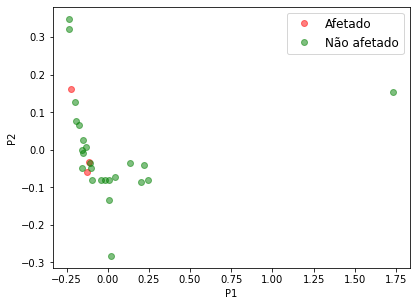
\includegraphics[scale=0.45]{images/base-de-dados-24.2-pca-2d-monthly-uf.png}
        \caption{Impacto mensal}
        \label{fig:resultados:base-de-dados-24.2-pca-2d-monthly-uf}
    \end{subfigure} ~ \quad
    \begin{subfigure}[b]{0.45\textwidth}
        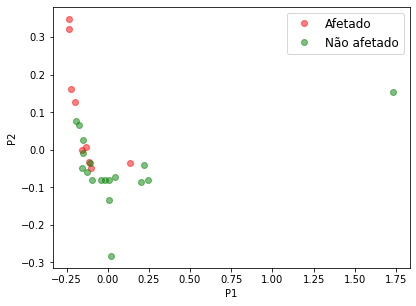
\includegraphics[scale=0.45]{images/base-de-dados-25.2-pca-2d-total-uf.png}
        \caption{Impacto total}
        \label{fig:resultados:base-de-dados-25.2-pca-2d-total-uf}
    \end{subfigure}
    \fdadospesquisa
\end{figure}

O conjunto de dados possui algum espalhamento nos dados, e parece ter algumas UFs um pouco mais distantes do restante. Porém, não existem regiões onde é clara a distinção de afetados e não afetados tanto para o impacto mensal quanto total. No caso do impacto total, existem UFs afetadas que parecem ocupar uma região próxima onde essas poderiam ser separadas linearmente, enquanto outras permanecem em uma região pouco divisível. Também é importante notar que ambos conjuntos de dados são desbalanceados, o que é um desafio para classificadores.

Ao aplicarmos classificadores sobre os dados foram obtidos os resultados ilustrados nas Figuras~\ref{fig:base-de-dados-24.1-confusion-matrix-monthly-uf}, \ref{fig:base-de-dados-24.1-confusion-matrix-total-uf1} e \ref{fig:base-de-dados-24.1-confusion-matrix-total-uf2}. A primeira se refere aos dados de impacto mensal e as seguintes ao impacto total, conforme descrito anteriormente. Para validação da técnica, foi utilizado o método \textit{leave-one-out}. 

Para a tentativa de classificação dos dados de UFs para impacto mensal, três classificadores tiveram o mesmo resultado: Random Forest, Regressão Logística, e SVC, onde todas as UFs foram classificadas como positivos. Já utilizando o classificador KNN, o resultado foi semelhante mas uma das UFs que deveria ser classificada como positivo foi agora classificada como negativo. Apesar de uma alta acurácia, o resultado não é interessante uma vez que temos uma grande quantidade de falsos positivos para todos os métodos, faltando generalização.

\begin{figure}[htb] 
    \centering 
    \caption{Matrizes de confusão para classificadores aplicados sobre dados de UFs para impacto mensal}
    \label{fig:base-de-dados-24.1-confusion-matrix-monthly-uf}
    \begin{subfigure}[b]{0.45\textwidth}
        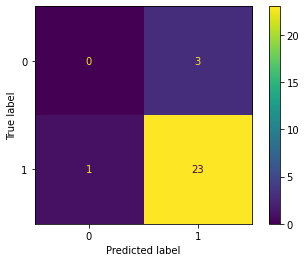
\includegraphics[scale=0.75]{images/base-de-dados-24.3-confusion-matrix-knn-monthly-uf.png}
        \caption{KNN}
        \label{fig:resultados:base-de-dados-24.3-confusion-matrix-knn-monthly-uf}
    \end{subfigure} ~ \quad
    \begin{subfigure}[b]{0.45\textwidth}
        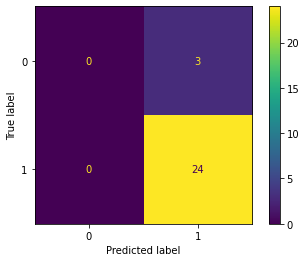
\includegraphics[scale=0.75]{images/base-de-dados-24.1-confusion-matrix-randomforest-monthly-uf.png}
        \caption{Random Forest, Regressão Logística, e SVC}
        \label{fig:resultados:base-de-dados-24.1-confusion-matrix-randomforest-monthly-uf}
    \end{subfigure}
    \fdadospesquisa
\end{figure}

Para os dados de impacto total, o resultado foi um pouco mais positivo. As maiores acurácias foram apresentadas pelos classificadores Regressão Logística e SVC, com cerca de 70\%, seguido de KNN com 66\% e Regressão Logística com 59\%. Evidentemente, a acurácia para este conjunto de dados desbalanceado esconde um grande problema dessa classificação, que é conseguir uma boa especificidade para este conjuntos de dados. Todos os classificadores tiveram problemas com a quantidade de falsos positivos e falsos negativos. Nenhum dos classificadores portanto conseguiu efetivamente alcançar uma generalização aceitável.

\begin{figure}[htb] 
    \centering 
    \caption{Matrizes de confusão para classificadores aplicados sobre dados de UFs para impacto total (Parte 1)}
    \label{fig:base-de-dados-24.1-confusion-matrix-total-uf1}
    \begin{subfigure}[b]{0.45\textwidth}
        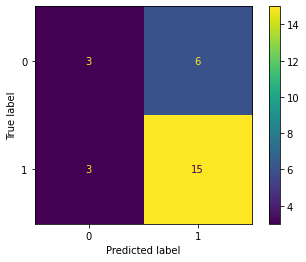
\includegraphics[scale=0.75]{images/base-de-dados-24.3-confusion-matrix-knn-total-uf.png}
        \caption{KNN}
        \label{fig:resultados:base-de-dados-24.3-confusion-matrix-knn-total-uf}
    \end{subfigure} ~ \quad
    \begin{subfigure}[b]{0.45\textwidth}
        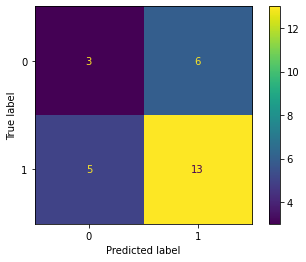
\includegraphics[scale=0.75]{images/base-de-dados-24.1-confusion-matrix-randomforest-total-uf.png}
        \caption{Random Forest}
        \label{fig:resultados:base-de-dados-24.1-confusion-matrix-randomforest-total-uf}
    \end{subfigure}
\end{figure}
\begin{figure}[htb] 
    \centering 
    \caption{Matrizes de confusão para classificadores aplicados sobre dados de UFs para impacto total (Parte 2)}
    \label{fig:base-de-dados-24.1-confusion-matrix-total-uf2}
    \begin{subfigure}[b]{0.45\textwidth}
        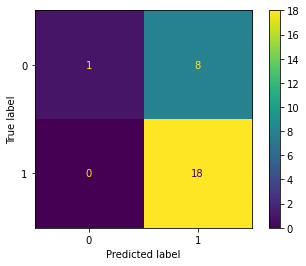
\includegraphics[scale=0.75]{images/base-de-dados-24.1-confusion-matrix-logisticregression-total-uf.png}
        \caption{Regressão Logística}
        \label{fig:resultados:base-de-dados-24.3-confusion-matrix-logisticregression-total-uf}
    \end{subfigure} ~ \quad
    \begin{subfigure}[b]{0.45\textwidth}
        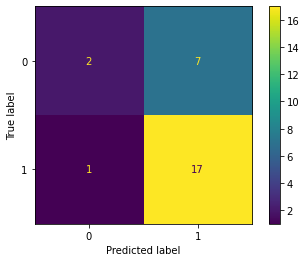
\includegraphics[scale=0.75]{images/base-de-dados-24.2-confusion-matrix-svc-total-uf.png}
        \caption{SVC}
        \label{fig:resultados:base-de-dados-24.1-confusion-matrix-svc-total-uf}
    \end{subfigure}
    \fdadospesquisa
\end{figure}

% \begin{table}[htb]
% \centering
% \caption{Métricas de classificação do impacto mensal de cada método para os dados de UFs}
% \label{tab:resultados:classification-report-monthly-uf}
% \begin{tabular}{l|r|rrrr}
% \toprule
% Método & Métrica & Negativos & Positivos & Média & \shortstack{Média\\ponderada} \\
% \midrule
% \multirow{4}{*}{KNN} & Precisão & 0.0000 &  0.8750 &  0.4375 &  0.7778 \\
%  & Recall   & 0.0000 &  0.8750 &  0.4375 &  0.7778 \\
%  & F1-Score & 0.0000 &  0.8750 &  0.4375 &  0.7778 \\
%  & Suporte  & 3.0000 & 24.0000 & 27.0000 & 27.0000 \\ \hline
% \multirow{4}{*}{Random forest} & Precisão & 0.0000 &  0.8889 &  0.4444 &  0.7901 \\
%  & Recall   & 0.0000 &  1.0000 &  0.5000 &  0.8889 \\
%  & F1-Score & 0.0000 &  0.9412 &  0.4706 &  0.8366 \\
%  & Suporte  & 3.0000 & 24.0000 & 27.0000 & 27.0000 \\ \hline
% \multirow{4}{*}{Regressão Logística} & Precisão & 0.0000 &  0.8889 &  0.4444 &  0.7901 \\
%  & Recall   & 0.0000 &  1.0000 &  0.5000 &  0.8889 \\
%  & F1-Score & 0.0000 &  0.9412 &  0.4706 &  0.8366 \\
%  & Suporte  & 3.0000 & 24.0000 & 27.0000 & 27.0000 \\ \hline
% \multirow{4}{*}{SVC} & Precisão & 0.0000 &  0.8889 &  0.4444 &  0.7901 \\
%  & Recall   & 0.0000 &  1.0000 &  0.5000 &  0.8889 \\
%  & F1-Score & 0.0000 &  0.9412 &  0.4706 &  0.8366 \\
%  & Suporte  & 3.0000 & 24.0000 & 27.0000 & 27.0000 \\
% \bottomrule
% \end{tabular}
% \fdadospesquisa
% \end{table}

\subsection{Dados de Seções}
\label{section:deteccao-impacto:secao}

Repetimos então a análise, construindo uma matriz agora usando os dados de seções, com os dados descritos na seção~\ref{section:metricas-redes:secao} junto das métricas de volume total, quantidade de transações, e valor médio de transações.

\begin{figure}[htb]
	\centering
    \caption{Percentual de variância explicada de cada componente principal para dados de seções}
    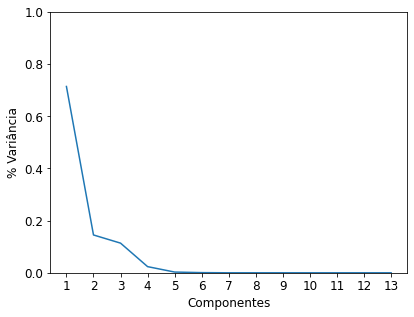
\includegraphics[scale=0.7]{images/base-de-dados-26.1-pca-components-monthly-secao.png}
    \label{fig:resultados:base-de-dados-24-pca-monthly-secao}
    \fdadospesquisa
\end{figure}

A matriz resultante possui uma linha para cada seção analisada e uma coluna para cada métrica, totalizando treze variáveis. Utilizamos também os dados de impacto mensal e total por seção descritos na seção~\ref{section:impacto:cenario-economico}.

\begin{table}[htb]
\centering
\caption{Direção de cada métrica em relação a cada uma das duas componentes principais para os dados de seções}
\label{tab:resultados:direcao-components-secao}
\begin{tabular}{l|rrrr}
\toprule
Componente & 1 & 2 \\
\midrule
Valor total                    &  0.4238 &  0.0153 \\
Quantidade de transações       &  0.3972 &  0.0648 \\
Valor médio por transação      & -0.0133 & -0.5534 \\
Grau                           &  0.0243 & -0.1738 \\
Coeficiente de agrupamento     &  0.3633 & -0.0632 \\
Excentricidade                 & -0.0702 & -0.0082 \\
Caminho mínimo médio           & -0.0195 &  0.1362 \\
Caminho mínimo médio ponderado & -0.0504 &  0.7709 \\
Centralidade de proximidade    &  0.0171 & -0.0829 \\
Centralidade de informação     &  0.0120 & -0.1816 \\
Centralidade de autovalores    &  0.4237 &  0.0396 \\
PageRank                       &  0.4121 &  0.0084 \\
Centralidade de intermediação  &  0.4151 &  0.0285 \\
\bottomrule
\end{tabular}
\fdadospesquisa
\end{table}

Assim como anteriormente, foi aplicada a análise das componentes principais dessa matriz. A Figura~\ref{fig:resultados:base-de-dados-24-pca-monthly-secao} mostra o percentual da variância total explicada pelo conjunto de dados para cada componente. Novamente, as duas primeiras componentes explicam a maior parte da variância do conjunto de dados.

\begin{figure}[htb] 
    \centering 
    \caption{Visualização dos dados de seções projetados sobre as duas componentes principais}
    \label{fig:resultados:pca-secao}
    \begin{subfigure}[b]{0.45\textwidth}
        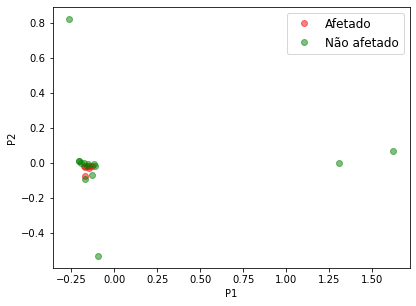
\includegraphics[scale=0.45]{images/base-de-dados-26.2-pca-2d-monthly-secao.png}
        \caption{Impacto mensal}
        \label{fig:resultados:base-de-dados-26.2-pca-2d-monthly-secao}
    \end{subfigure} ~ \quad
    \begin{subfigure}[b]{0.45\textwidth}
        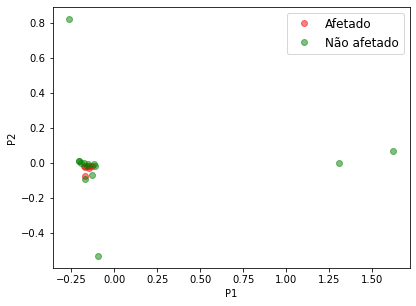
\includegraphics[scale=0.45]{images/base-de-dados-27.2-pca-2d-total-secao.png}
        \caption{Impacto total}
        \label{fig:resultados:base-de-dados-27.2-pca-2d-total-secao}
    \end{subfigure}
    \fdadospesquisa
\end{figure}

A seguir, na Tabela~\ref{tab:resultados:direcao-components-secao}, é descrita a direção de cara variável em relação às duas principais componentes. O valor total novamente tem uma participação importante, mas as métricas de centralidade de autovalores, \textit{pagerank}, e centralidade de intermediação apresentam também magnitude significativa em relação à primeira componente, enquanto as maiores magnitudes para a segundo componentes pertencem às váriáveis valor médio por transação e caminho mínimo médio ponderado.

A Figura~\ref{fig:resultados:pca-secao} apresenta o espalhamento dos dados projetos sobre as duas componentes principais representando o impacto mensal e total. É possível ver que os dados são pouco espalhados e se concentram em uma região principal do espaço de variáveis, além de possuir quatro seções distantes com um aparente comportamento de \textit{outliers}. Novamente, os dados são bastante desbalanceados.

\begin{figure}[htb] 
    \centering 
    \caption{Matrizes de confusão para classificadores aplicados sobre dados de seções para impacto mensal}
    \label{fig:base-de-dados-24.1-confusion-matrix-monthly-secao}
    \begin{subfigure}[b]{0.45\textwidth}
        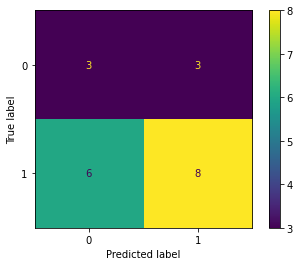
\includegraphics[scale=0.75]{images/base-de-dados-24.3-confusion-matrix-knn-monthly-secao.png}
        \caption{KNN}
        \label{fig:resultados:base-de-dados-24.3-confusion-matrix-knn-monthly-secao}
    \end{subfigure} ~ \quad
    \begin{subfigure}[b]{0.45\textwidth}
        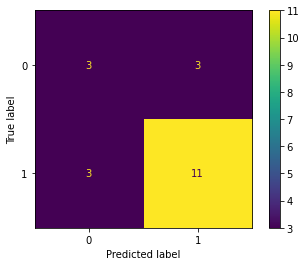
\includegraphics[scale=0.75]{images/base-de-dados-24.1-confusion-matrix-randomforest-monthly-secao.png}
        \caption{Random Forest}
        \label{fig:resultados:base-de-dados-24.1-confusion-matrix-randomforest-monthly-secao}
    \end{subfigure} \\
    \begin{subfigure}[b]{0.45\textwidth}
        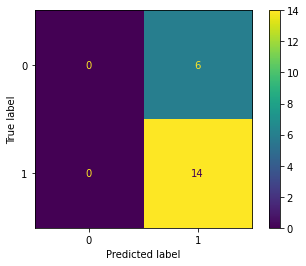
\includegraphics[scale=0.75]{images/base-de-dados-24.1-confusion-matrix-logisticregression-monthly-secao.png}
        \caption{Regressão Logística}
        \label{fig:resultados:base-de-dados-24.3-confusion-matrix-logisticregression-monthly-secao}
    \end{subfigure} ~ \quad
    \begin{subfigure}[b]{0.45\textwidth}
        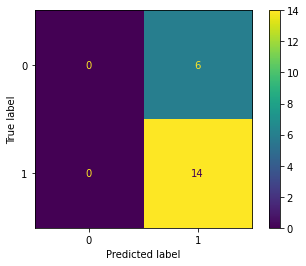
\includegraphics[scale=0.75]{images/base-de-dados-24.2-confusion-matrix-svc-monthly-secao.png}
        \caption{SVC}
        \label{fig:resultados:base-de-dados-24.1-confusion-matrix-svc-monthly-secao}
    \end{subfigure}
    \fdadospesquisa
\end{figure}

\begin{figure}[htb] 
    \centering 
    \caption{Matrizes de confusão para classificadores aplicados sobre dados de seções para impacto total}
    \label{fig:base-de-dados-24.1-confusion-matrix-total-secao}
    \begin{subfigure}[b]{0.45\textwidth}
        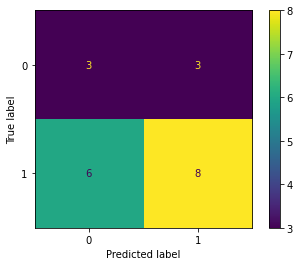
\includegraphics[scale=0.75]{images/base-de-dados-24.3-confusion-matrix-knn-total-secao.png}
        \caption{KNN}
        \label{fig:resultados:base-de-dados-24.3-confusion-matrix-knn-total-secao}
    \end{subfigure} ~ \quad
    \begin{subfigure}[b]{0.45\textwidth}
        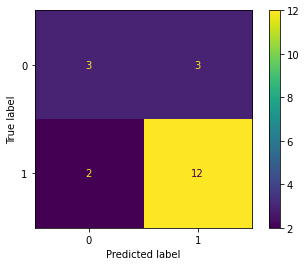
\includegraphics[scale=0.75]{images/base-de-dados-24.1-confusion-matrix-randomforest-total-secao.png}
        \caption{Random Forest}
        \label{fig:resultados:base-de-dados-24.1-confusion-matrix-randomforest-total-secao}
    \end{subfigure} \\
    \begin{subfigure}[b]{0.45\textwidth}
        \includegraphics[scale=0.75]{images/base-de-dados-24.1-confusion-matrix-logisticregression-total-secao.png}
        \caption{Regressão Logística}
        \label{fig:resultados:base-de-dados-24.3-confusion-matrix-logisticregression-total-secao}
    \end{subfigure} ~ \quad
    \begin{subfigure}[b]{0.45\textwidth}
        \includegraphics[scale=0.75]{images/base-de-dados-24.2-confusion-matrix-svc-total-secao.png}
        \caption{SVC}
        \label{fig:resultados:base-de-dados-24.1-confusion-matrix-svc-total-secao}
    \end{subfigure}
    \fdadospesquisa
\end{figure}

Foram aplicados também classificadores sobre os dados, que são ilustrados nas Figuras~\ref{fig:base-de-dados-24.1-confusion-matrix-monthly-secao} e \ref{fig:base-de-dados-24.1-confusion-matrix-total-secao}, referentes ao impacto mensal e total respectivamente. Para a validação foi novamente utilizada a técnica \textit{leave-one-out}.

Novamente, os classificadores não foram capazes de apresentar boa generalização sobre os dados, sendo que dois deles classificaram todas as seções como afetadas pela crise. O classificador KNN apresentou baixa precisão, com uma alta taxa de falsos positivos. E o classificador Random Forest apresentou um resultado razoável, com uma acurácia de 70\%, precisão de 78\% e especificidade de 50\%.

\subsection{Dados de CNAEs}
\label{section:deteccao-impacto:cnae}

Por fim, aplicamos a mesma técnica anterior sobre os dados de CNAEs.

\begin{figure}[htb]
	\centering
    \caption{Percentual de variância explicada de cada componente principal para dados de CNAEs}
    \includegraphics[scale=0.7]{images/base-de-dados-28.1-pca-components-monthly-cnae.png}
    \label{fig:resultados:base-de-dados-24-pca-monthly-cnae}
    \fdadospesquisa
\end{figure}

Montamos uma matriz novamente agregando os dados de volume total transacionado, quantidade de transações, valor médio de transações, seção do CNAE (discretizada), e as métricas de redes da seção~\ref{section:metricas-redes:cnae}, totalizando catorze variáveis.

\begin{table}[htb]
\centering
\caption{Direção de cada métrica em relação a cada uma das duas componentes principais para os dados de CNAEs}
\label{tab:resultados:direcao-components-cnae}
\begin{tabular}{l|rrrr}
\toprule
Componente & 1 & 2 & 3 & 4 \\
\midrule
Seção                          &  0.5035 & -0.0108 &  0.0966 &  0.0441 \\
Valor total                    &  0.4563 &  0.3150 & -0.0079 & -0.1132 \\
Quantidade de transações       &  0.0612 & -0.4170 &  0.6541 &  0.1840 \\
Valor médio por transação      &  0.1895 & -0.2848 & -0.3259 &  0.0631 \\
Grau                           &  0.1765 & -0.3230 &  0.3309 &  0.1040 \\
Coeficiente de agrupamento     & -0.0217 &  0.0357 &  0.0442 & -0.0124 \\
Excentricidade                 & -0.0328 &  0.0529 &  0.0559 & -0.0012 \\
Caminho mínimo médio           & -0.0295 &  0.3470 & -0.0146 &  0.9292 \\
Caminho mínimo médio ponderado &  0.0388 & -0.0607 & -0.0697 &  0.0092 \\
Centralidade de proximidade    &  0.0207 & -0.0689 & -0.0039 & -0.0521 \\
Centralidade de informação     &  0.4090 &  0.4709 &  0.1726 & -0.1805 \\
Centralidade de autovalores    &  0.4696 & -0.1466 &  0.0038 &  0.0944 \\
PageRank                       &  0.2737 & -0.3887 & -0.5499 &  0.1673 \\
Centralidade de intermediação  & -0.0225 &  0.1185 & -0.0681 &  0.0283 \\
\bottomrule
\end{tabular}
\fdadospesquisa
\end{table}

A Figura~\ref{fig:resultados:base-de-dados-24-pca-monthly-cnae} apresenta o percentual da variância explicada pelo conjunto de dados para cada componente principal dessa matriz. Ao contrário dos conjuntos anteriores, há maior distribuição da variância explicada por entre as componentes. São necessárias agora quatro componentes principais para totalizar 80.6\% da variância total do conjunto de dados.

A Tabela~\ref{tab:resultados:direcao-components-cnae} mostra a direção de cada variável em relação a cada uma das quatro componentes principais. Algumas métricas já citadas nas análises anteriores novamente se sobressaem: valor total, quantidade de transações, centralidade de informação, centralidade de autovalores, \textit{pagerank}. A variável seção, adicionada para melhorar o espalhamento dos dados, também tem participação importante principalmente na primeira componente principal.

A Figura~\ref{fig:resultados:base-de-dados-24-pca-monthly-cnae} mostra o espalhamento dos dados projetados sobre as duas componentes principais em relação ao impacto mensal e total. É possível novamente ver que não há um espalhamento significativo, com exceção de alguns \textit{outliers}, e as duas classes se sobrepõem uma a outra sem regiões bem definidas. O conjunto considerando impacto mensal é bastante desbalanceado, enquanto o conjunto que considera impacto total é menos desbalanceado.

\begin{figure}[htb] 
    \centering 
    \caption{Visualização dos dados de CNAEs projetados sobre as duas componentes principais}
    \label{fig:resultados:pca-cnae}
    \begin{subfigure}[b]{0.45\textwidth}
        \includegraphics[scale=0.45]{images/base-de-dados-28.2-pca-2d-monthly-cnae.png}
        \caption{Impacto mensal}
        \label{fig:resultados:base-de-dados-24.2-pca-2d-monthly-cnae}
    \end{subfigure} ~ \quad
    \begin{subfigure}[b]{0.45\textwidth}
        \includegraphics[scale=0.45]{images/base-de-dados-28.2-pca-2d-total-cnae.png}
        \caption{Impacto total}
        \label{fig:resultados:base-de-dados-25.2-pca-2d-total-cnae}
    \end{subfigure}
    \fdadospesquisa
\end{figure}

Mais uma vez aplicamos classificadores sobre os dados para identificação do impacto mensal e total. Desta vez, dado o tamanho do dataset utilizados a técnica k-fold estratificado para validarmos os dados obtidos através dos classificadores. As Figuras~\ref{fig:resultados:classification-monthly-cnae} e \ref{fig:resultados:classification-total-cnae} mostram os resultados obtidos, através das matrizes de confusão e curva ROC.

Para o conjunto de dados de impacto mensal, novamente os classificadores falharam em identificar verdadeiros negativos. O classificador que melhor conseguiu generalizar os dados foi novamente Random Forest, com uma precisão de 95\% mas uma especificidade de apenas 12\%. Também para o conjunto de dados de impacto total, significativamente mais balanceado, os resultados apresentaram pouca generalização. Todos os métodos apresentaram uma alta taxa de falsos positivos e negativos.

\begin{figure}[htb] 
    \centering 
    \caption{Resultado das tentativas de classificação para cada método aplicado sobre dados de CNAEs para impacto mensal}
    \label{fig:resultados:classification-monthly-cnae} 
    \begin{subfigure}[b]{0.45\textwidth}
        \includegraphics[scale=0.55]{images/base-de-dados-28.3.5-confusion-matrix-knn-monthly-cnae.png}
        \caption{Matriz de confusão para KNN}
        \label{fig:resultados:base-de-dados-28.3.5-confusion-matrix-knn-monthly-cnae}
    \end{subfigure} ~ \quad
    \begin{subfigure}[b]{0.45\textwidth}
        \includegraphics[scale=0.55]{images/base-de-dados-28.3.6-roc-curve-knn-monthly-cnae.png}
        \caption{Curva ROC para KNN}
        \label{fig:resultados:base-de-dados-28.3.6-roc-curve-knn-monthly-cnae}
    \end{subfigure} ~ \\
    \begin{subfigure}[b]{0.45\textwidth}
        \includegraphics[scale=0.55]{images/base-de-dados-28.3.1-confusion-matrix-randomforest-monthly-cnae.png}
        \caption{Matriz de confusão para Random Forest}
        \label{fig:resultadosbase-de-dados-28.3.1-confusion-matrix-randomforest-monthly-cnae}
    \end{subfigure} ~ \quad
    \begin{subfigure}[b]{0.45\textwidth}
        \includegraphics[scale=0.55]{images/base-de-dados-28.3.2-roc-curve-randomforest-monthly-cnae.png}
        \caption{Curva ROC para Random Forest}
        \label{fig:resultados:base-de-dados-28.3.2-roc-curve-randomforest-monthly-cnae}
    \end{subfigure} ~ \\
    \begin{subfigure}[b]{0.45\textwidth}
        \includegraphics[scale=0.55]{images/base-de-dados-28.3.7-confusion-matrix-logregression-monthly-cnae.png}
        \caption{Matriz de confusão para Regressão logística}
        \label{fig:resultados:base-de-dados-28.3.7-confusion-matrix-logregression-monthly-cnae}
    \end{subfigure} ~ \quad
    \begin{subfigure}[b]{0.45\textwidth}
        \includegraphics[scale=0.55]{images/base-de-dados-28.3.8-roc-curve-logregression-monthly-cnae.png}
        \caption{Curva ROC para Regressão Logística}
        \label{fig:resultados:base-de-dados-28.3.8-roc-curve-logregression-monthly-cnae}
    \end{subfigure} ~ \\
        \begin{subfigure}[b]{0.45\textwidth}
        \includegraphics[scale=0.55]{images/base-de-dados-28.3.3-confusion-matrix-svc-monthly-cnae.png}
        \caption{Matriz de confusão para SVC}
        \label{fig:resultados:base-de-dados-28.3.3-confusion-matrix-svc-monthly-cnae}
    \end{subfigure} ~ \quad
    \begin{subfigure}[b]{0.45\textwidth}
        \includegraphics[scale=0.55]{images/base-de-dados-28.3.4-roc-curve-svc-monthly-cnae.png}
        \caption{Curva ROC para SVC}
        \label{fig:resultados:base-de-dados-28.3.4-roc-curve-svc-monthly-cnae}
    \end{subfigure}
    \fdadospesquisa
\end{figure}

\begin{figure}[htb] 
    \centering 
    \caption{Resultado das tentativas de classificação para cada método aplicado sobre dados de CNAEs para impacto total}
    \label{fig:resultados:classification-total-cnae} 
    \begin{subfigure}[b]{0.45\textwidth}
        \includegraphics[scale=0.55]{images/base-de-dados-28.4.5-confusion-matrix-knn-total-cnae.png}
        \caption{Matriz de confusão para KNN}
        \label{fig:resultados:base-de-dados-28.3.5-confusion-matrix-knn-total-cnae}
    \end{subfigure} ~ \quad
    \begin{subfigure}[b]{0.45\textwidth}
        \includegraphics[scale=0.55]{images/base-de-dados-28.4.6-roc-curve-knn-total-cnae.png}
        \caption{Curva ROC para KNN}
        \label{fig:resultados:base-de-dados-28.3.6-roc-curve-knn-total-cnae}
    \end{subfigure} ~ \\
    \begin{subfigure}[b]{0.45\textwidth}
        \includegraphics[scale=0.55]{images/base-de-dados-28.4.1-confusion-matrix-randomforest-total-cnae.png}
        \caption{Matriz de confusão para Random Forest}
        \label{fig:resultadosbase-de-dados-28.3.1-confusion-matrix-randomforest-total-cnae}
    \end{subfigure} ~ \quad
    \begin{subfigure}[b]{0.45\textwidth}
        \includegraphics[scale=0.55]{images/base-de-dados-28.4.2-roc-curve-randomforest-total-cnae.png}
        \caption{Curva ROC para Random Forest}
        \label{fig:resultados:base-de-dados-28.3.2-roc-curve-randomforest-total-cnae}
    \end{subfigure} ~ \\
    \begin{subfigure}[b]{0.45\textwidth}
        \includegraphics[scale=0.55]{images/base-de-dados-28.4.7-confusion-matrix-logregression-total-cnae.png}
        \caption{Matriz de confusão para Regressão logística}
        \label{fig:resultados:base-de-dados-28.3.7-confusion-matrix-logregression-total-cnae}
    \end{subfigure} ~ \quad
    \begin{subfigure}[b]{0.45\textwidth}
        \includegraphics[scale=0.55]{images/base-de-dados-28.4.8-roc-curve-logregression-total-cnae.png}
        \caption{Curva ROC para Regressão Logística}
        \label{fig:resultados:base-de-dados-28.3.8-roc-curve-logregression-total-cnae}
    \end{subfigure} ~ \\
    \begin{subfigure}[b]{0.45\textwidth}
        \includegraphics[scale=0.55]{images/base-de-dados-28.4.3-confusion-matrix-svc-total-cnae.png}
        \caption{Matriz de confusão para SVC}
        \label{fig:resultados:base-de-dados-28.3.3-confusion-matrix-svc-total-cnae}
    \end{subfigure} ~ \quad
    \begin{subfigure}[b]{0.45\textwidth}
        \includegraphics[scale=0.55]{images/base-de-dados-28.4.4-roc-curve-svc-total-cnae.png}
        \caption{Curva ROC para SVC}
        \label{fig:resultados:base-de-dados-28.3.4-roc-curve-svc-total-cnae}
    \end{subfigure} ~ \\
    \fdadospesquisa
\end{figure}

\subsection{Conclusões}
\label{section:deteccao-impacto:conclusoes}

Nesta seção, montamos uma tentativa de classificação de entidades impactadas e não impactadas pela crise causada pela pandemia. Foram utilizadas três abordagens, por UF, por seção, e por CNAE, e fizemos um estudo da variância e de como os dados se espalham.

Já na análise de componentes principais, foi possível perceber para os três conjuntos de dados que eles não possuem um espalhamento adequado para que um classificador esteja apto a separar os conjuntos de dados. Sendo que os classificadores escolhidos foram utilizados justamente para tentar utilizar diferentes abordagens de classificação.

Foram utilizadas também algumas técnicas para tentar reduzir o \textit{overfitting} nos dados: utilizamos a análise de componentes principais para selecionar apenas dimensões de maior taxa de explicabilidade, utilizamos técnicas de discretização dos dados para tentar uma melhor separação dos dados, e algumas variáveis não apresentadas aqui também foram inseridas no conjunto de dados e depois removidas ou por ser redundante com alguma outra variável, ou por ser insuficiente para um melhor espalhamento dos dados.

O resultado aqui obtido não o ideal, mas de forma alguma eles significam que seja impossível fazer um classificador que esteja apto a esses conjuntos de dados. Outros classificadores não utilizados aqui podem ter a capacidade de obter melhores resultados, e até mesmo os classificadores que foram utilizados podem apresentar resultados melhores com outros tratamentos aplicados aos dados ou com a adição de novas variáveis.


\chapter{Conclusão}
\label{chapter:conclusão}

\section{Pontos positivos e negativos}

pros:

métricas de redes contribuíram positivamente para a identificação de crises tanto em um grafo simples (UF) quanto mais complexos (CNAE)

cons:

aplicacao sobre dados de empresas nao foi possivel

\section{Próximos passos}

usar outros documentos fiscais

uso de algoritmos mais escaláveis ou processamento distribuido


% ---
% Finaliza a parte no bookmark do PDF, para que se inicie o bookmark na raiz
% ---
\bookmarksetup{startatroot}% 
% ---

% ----------------------------------------------------------
% ELEMENTOS PÓS-TEXTUAIS
% ----------------------------------------------------------
\postextual

% ----------------------------------------------------------
% Referências bibliográficas
% ----------------------------------------------------------
\bibliography{references}

% ---------------------------------------------------------------------
% GLOSSÁRIO
% ---------------------------------------------------------------------

% Arquivo que contém as definições que vão aparecer no glossário
\newword{WYSIWYG}{``What You See Is What You Get''  ou ``O que você vê é o que você obtém''.  Recurso tem por objetivo permitir que um documento, enquanto manipulado na tela, tenha a mesma aparência de sua utilização, usualmente sendo considerada final. Isso facilita para o desenvolvedor que pode trabalhar visualizando a aparência do documento sem precisar salvar em vários momentos e abrir em um \textit{software} separado de visualização}
\newword{Framework}{é uma abstração que une códigos comuns entre vários projetos de \textit{software} provendo uma funcionalidade genérica. \textit{Frameworks} são projetados com a intenção de facilitar o desenvolvimento de \textit{software}, habilitando designers e programadores a gastarem mais tempo determinando as exigências do \textit{software} do que com detalhes de baixo nível do sistema}

\newword{Template}{é um documento sem conteúdo, com apenas a apresentação visual (apenas cabeçalhos por exemplo) e instruções sobre onde e qual tipo de conteúdo deve entrar a cada parcela da apresentação}

\newword{Padrões de projeto}{ou \textit{Design Pattern}, descreve uma solução geral reutilizável para um problema recorrente no desenvolvimento de sistemas de \textit{software} orientados a objetos. Não é um código final, é uma descrição ou modelo de como resolver o problema do qual trata, que pode ser usada em muitas situações diferentes}

\newword{Web}{Sinônimo mais conhecido de \textit{World Wide Web} (WWW). É a interface gráfica da Internet que torna os serviços disponíveis totalmente transparentes para o usuário e ainda possibilita a manipulação multimídia da informação}

% Comando para incluir todas as definições do arquivo glossario.tex
\glsaddall
% Impressão do glossário
\printglossaries

% ----------------------------------------------------------
% Apêndices
% ----------------------------------------------------------

% ---
% Inicia os apêndices
% ---
\begin{apendicesenv}

    \chapter{Armazém de Dados}
    \label{chapter:armazem-de-dados}
    
Neste apêndice, será descrito parte da arquitetura de ingestão de documentos fiscais utilizado pela empresa parceira.

\section{Arquitetura de Ingestão}

A Arquivei, empresa parceira deste trabalho, possui em sua plataforma diversos fluxos de ingestão de documentos fiscais. O usuário pode fazer o upload de documentos por diversos meios, sendo eles:

\begin{itemize}
    \item Upload via plataforma \textit{web}
    \item Upload de arquivos zip via plataforma \textit{web}
    \item Envio por email
    \item Através do Sincroniza Notas, um produto instalável que faz integrações com ERPs e outros sistemas contábeis
    \item Através de consulta automatizada utilizando certificado digital A1
    \item Através do Modulo de Segurança da Arquivei que utiliza uma integração \textit{web} para fazer a consulta via certificado digital A3
\end{itemize}

O fluxo de consulta automatizada é especialmente importante porque é por este fluxo que são recebidos os documentos vindos da Secretaria da Fazenda. O sistema de consulta lida de forma eficiente com os \textit{web services} de forma a garantir que o cliente tenha acesso a todas as informações disponíveis, da forma mais consistente possível. Estes documentos possuem um grau de confiabilidade maior em relação aos demais, uma vez que os documentos recebidos através dos clientes podem ter inconsistências ou incompletudes por problemas de comunicação e integração. Essas inconsistências podem apresentar ruídos em análises de dados, uma vez que nem todas as informações disponíveis no documento fiscal são checadas pela Secretaria da Fazenda e as alterações dos mesmos ocorrem através de documentos específicos, chamadas Cartas de Correção, que são de difícil processamento.

Todos esses fluxos passam por um fluxo centralizado de tratamento de dados, que garante certa consistência e integridade. Os documentos coletados são então enviados a um sistema chamado Plataforma de Documentos Fiscais, descrito a seguir.

\section{Plataforma de DFe}

A Plataforma de Documentos Fiscais é o sistema responsável por armazenar os documentos de forma segura, consistente, e disponível. Esta plataforma usa o conceito de Fonte Única de Verdade para construir um conjunto de sistemas responsável por tratar os dados de documentos fiscais de forma centralizada e consistente.

A plataforma disponibiliza uma série de APIs para ingestão síncrona, ingestão assíncrona, e disponibilização dos dados. Os clientes da plataforma são times internos da Arquivei, responsáveis por construir diferentes produtos, que se usam das funcionalidades da mesma para agilizar e melhorar suas entregas.

\section{Armazém de Dados}

Uma das interfaces da Plataforma de DFe é um protocolo de replicação de dados chamado Change Data Capture (CDC), em tradução livre Captura de Modificações de Dados, que é um protocolo capaz de transmitir mudanças feitas em um banco de dados para sistemas externos de forma a possibilitar a geração de visualizações.

Visualizações são bancos de dados de propósito específico criados a partir de uma Fonte Única de Verdade, visando atender demandas específicas. Uma empresa pode escolher ter visualizações analíticas, visualizações de índice-invertido, ou visualizações transacionais, por exemplo. Cada visualização irá disponibilizar os dados através de um novo protocolo ou de uma nova modelagem, conforme as demandas da empresa ou organização.

Uma visualização utilizada são armazéns de dados. O armazém de dados da Arquivei é construído a partir do CDC visando disponibilizar os dados da base de dados para análise. Através do armazém de dados de documentos fiscais foi possível obter os dados para este trabalho. O armazém também armazena dados coletados de base de dados externas que tenham alguma interação com os dados transacionais ou de documentos fiscais.

    
    \chapter{Tecnologias Utilizadas}
    \label{chapter:tecnologias-utilizadas}
    
bigquery (sql, tipos de dados), biblotecas (networkx, matplotlib, sklearn, outras libs), ferramentas de processamento paralelo, jupyter/google notebooks

    
    \chapter{CFOP - Código Financeiro de Operações}
    \label{chapter:cfop}
    
descrição do que é CFOP e quais foram utilizados e excluídos


\end{apendicesenv}
% ---


% ----------------------------------------------------------
% Anexos
% ----------------------------------------------------------

% ---
% Inicia os anexos
% ---
\begin{anexosenv}

    \chapter{Trabalhos Relacionados Relevantes}
    \label{chapter:trabalhos-relevantes}
    
\begin{description}
 \item[\url{http://www.google.com}] Algum link relevante
\end{description}


\end{anexosenv}
% ---

\end{document}